\documentclass{article} % For LaTeX2e
\usepackage[utf8]{inputenc}
\usepackage{times}
\usepackage{url}

\usepackage{graphicx}
\usepackage{amsmath}
\usepackage{amssymb}
\usepackage{algorithm,algorithmic}
\usepackage{amsfonts,bm}
\usepackage{bbm}
\usepackage{eqparbox}
\renewcommand{\algorithmiccomment}[1]{\eqparbox{COMMENT}{// #1}}
\usepackage{wrapfig}
\usepackage{url}
\usepackage{lipsum}
\usepackage{multicol}
\usepackage{multirow}
\usepackage{xcolor}
\usepackage{colortbl}
\usepackage{enumitem}
\usepackage{booktabs}
%\usepackage[font=small]{caption}
\usepackage{natbib}
\usepackage{latexml}
\newif\iflatexml
\latexmltrue

\newif\ifarxiv
\arxivtrue
% !TEX root = ../main.tex
% To remove comments
\newif\ifcomments
\commentstrue
% \commentsfalse

% \arxivfalse

\newcommand{\mr}[2]{\multirow{#1}{*}{#2}}%
\newcommand{\authcomment}[3]{\ifcomments {\color{#2} [#1: #3]} \else \fi}

% Pick your favorite color :)
\newcommand{\JL}[1]{\authcomment{JL}{brown}{#1}}
\newcommand{\XP}[1]{\authcomment{XP}{green}{#1}}
\newcommand{\MR}[1]{\authcomment{MR}{orange}{#1}}
\newcommand{\MRedit}[1]{\color{gray}{#1}}
\newcommand{\RZ}[1]{\authcomment{RZ}{red}{#1}}
\newcommand{\JS}[1]{\authcomment{JS}{teal}{#1}}
\newcommand{\ET}[1]{\authcomment{ET}{purple}{#1}}
\newcommand{\KCW}[1]{\authcomment{KCW}{magenta}{#1}}


\ifarxiv
\newcommand{\savespace}[1]{}
\newcommand{\savespaceeqn}{}
\newcommand{\savespacefig}{}
\newcommand{\savespacefigtop}[1]{}
\newcommand{\savespacebeforesection}{}
\newcommand{\savespacebeforeitem}{}
\else
\newcommand{\savespaceeqn}{\vskip -0.5cm}
\newcommand{\savespacefigtop}[1]{\vspace{#1}}
% \newcommand{\savespacefigtop}[1]{}
\newcommand{\savespace}[1]{\vspace{#1}}
\newcommand{\savespacefig}{}
\newcommand{\savespacebeforesection}{\vspace{-0.1in}}
\newcommand{\savespacebeforeitem}{\vspace{-0.03in}}
\fi

\newcommand{\gr}{\cellcolor[gray]{0.9}}
\newcommand{\gt}[1]{\textcolor{red}{#1}}
\newcommand{\sr}{\scriptsize}

\usepackage{xspace}

% \ifarxiv
\newcommand*{\eg}{e.g.\@\xspace}
\newcommand*{\ie}{i.e.\@\xspace}

\makeatletter
\newcommand*{\etc}{%
    \@ifnextchar{.}%
        {etc}%
        {etc.\@\xspace}%
}
\makeatother
% \fi
\newcommand{\mc}{\multicolumn}
\newcommand{\mrr}{\multirow}
\newcommand{\ul}{\underline}
\newcommand{\uftpn}{UFTE}
\newcommand{\uftsa}{UFTA}
\newcommand{\cm}{\checkmark}

\definecolor{red}{RGB}{255,73,92}
\definecolor{blue}{RGB}{37,110,255}
\definecolor{violet}{RGB}{70,35,122}
\definecolor{green}{RGB}{61,220,151}

\newcommand{\taskname}{FSAL}
\newcommand{\titlelower}{few-shot attribute learning}
% \newcommand{\titleupper}{Few-Shot Attribute Learning}

%%%%% NEW MATH DEFINITIONS %%%%%

\usepackage{amsmath,amsfonts,bm}

% Mark sections of captions for referring to divisions of figures
\newcommand{\figleft}{{\em (Left)}}
\newcommand{\figcenter}{{\em (Center)}}
\newcommand{\figright}{{\em (Right)}}
\newcommand{\figtop}{{\em (Top)}}
\newcommand{\figbottom}{{\em (Bottom)}}
\newcommand{\captiona}{{\em (a)}}
\newcommand{\captionb}{{\em (b)}}
\newcommand{\captionc}{{\em (c)}}
\newcommand{\captiond}{{\em (d)}}

% Highlight a newly defined term
\newcommand{\newterm}[1]{{\bf #1}}


% Figure reference, lower-case.
\def\figref#1{figure~\ref{#1}}
% Figure reference, capital. For start of sentence
\def\Figref#1{Figure~\ref{#1}}
\def\twofigref#1#2{figures \ref{#1} and \ref{#2}}
\def\quadfigref#1#2#3#4{figures \ref{#1}, \ref{#2}, \ref{#3} and \ref{#4}}
% Section reference, lower-case.
\def\secref#1{section~\ref{#1}}
% Section reference, capital.
\def\Secref#1{Section~\ref{#1}}
% Reference to two sections.
\def\twosecrefs#1#2{sections \ref{#1} and \ref{#2}}
% Reference to three sections.
\def\secrefs#1#2#3{sections \ref{#1}, \ref{#2} and \ref{#3}}
% Reference to an equation, lower-case.
\def\eqref#1{equation~\ref{#1}}
% Reference to an equation, upper case
\def\Eqref#1{Equation~\ref{#1}}
% A raw reference to an equation---avoid using if possible
\def\plaineqref#1{\ref{#1}}
% Reference to a chapter, lower-case.
\def\chapref#1{chapter~\ref{#1}}
% Reference to an equation, upper case.
\def\Chapref#1{Chapter~\ref{#1}}
% Reference to a range of chapters
\def\rangechapref#1#2{chapters\ref{#1}--\ref{#2}}
% Reference to an algorithm, lower-case.
\def\algref#1{algorithm~\ref{#1}}
% Reference to an algorithm, upper case.
\def\Algref#1{Algorithm~\ref{#1}}
\def\twoalgref#1#2{algorithms \ref{#1} and \ref{#2}}
\def\Twoalgref#1#2{Algorithms \ref{#1} and \ref{#2}}
% Reference to a part, lower case
\def\partref#1{part~\ref{#1}}
% Reference to a part, upper case
\def\Partref#1{Part~\ref{#1}}
\def\twopartref#1#2{parts \ref{#1} and \ref{#2}}

\def\ceil#1{\lceil #1 \rceil}
\def\floor#1{\lfloor #1 \rfloor}
\def\1{\bm{1}}
\newcommand{\train}{\mathcal{D}}
\newcommand{\valid}{\mathcal{D_{\mathrm{valid}}}}
\newcommand{\test}{\mathcal{D_{\mathrm{test}}}}

\def\eps{{\epsilon}}


% Random variables
\def\reta{{\textnormal{$\eta$}}}
\def\ra{{\textnormal{a}}}
\def\rb{{\textnormal{b}}}
\def\rc{{\textnormal{c}}}
\def\rd{{\textnormal{d}}}
\def\re{{\textnormal{e}}}
\def\rf{{\textnormal{f}}}
\def\rg{{\textnormal{g}}}
\def\rh{{\textnormal{h}}}
\def\ri{{\textnormal{i}}}
\def\rj{{\textnormal{j}}}
\def\rk{{\textnormal{k}}}
\def\rl{{\textnormal{l}}}
% rm is already a command, just don't name any random variables m
\def\rn{{\textnormal{n}}}
\def\ro{{\textnormal{o}}}
\def\rp{{\textnormal{p}}}
\def\rq{{\textnormal{q}}}
\def\rr{{\textnormal{r}}}
\def\rs{{\textnormal{s}}}
\def\rt{{\textnormal{t}}}
\def\ru{{\textnormal{u}}}
\def\rv{{\textnormal{v}}}
\def\rw{{\textnormal{w}}}
\def\rx{{\textnormal{x}}}
\def\ry{{\textnormal{y}}}
\def\rz{{\textnormal{z}}}

% Random vectors
\def\rvepsilon{{\mathbf{\epsilon}}}
\def\rvtheta{{\mathbf{\theta}}}
\def\rva{{\mathbf{a}}}
\def\rvb{{\mathbf{b}}}
\def\rvc{{\mathbf{c}}}
\def\rvd{{\mathbf{d}}}
\def\rve{{\mathbf{e}}}
\def\rvf{{\mathbf{f}}}
\def\rvg{{\mathbf{g}}}
\def\rvh{{\mathbf{h}}}
\def\rvu{{\mathbf{i}}}
\def\rvj{{\mathbf{j}}}
\def\rvk{{\mathbf{k}}}
\def\rvl{{\mathbf{l}}}
\def\rvm{{\mathbf{m}}}
\def\rvn{{\mathbf{n}}}
\def\rvo{{\mathbf{o}}}
\def\rvp{{\mathbf{p}}}
\def\rvq{{\mathbf{q}}}
\def\rvr{{\mathbf{r}}}
\def\rvs{{\mathbf{s}}}
\def\rvt{{\mathbf{t}}}
\def\rvu{{\mathbf{u}}}
\def\rvv{{\mathbf{v}}}
\def\rvw{{\mathbf{w}}}
\def\rvx{{\mathbf{x}}}
\def\rvy{{\mathbf{y}}}
\def\rvz{{\mathbf{z}}}

% Elements of random vectors
\def\erva{{\textnormal{a}}}
\def\ervb{{\textnormal{b}}}
\def\ervc{{\textnormal{c}}}
\def\ervd{{\textnormal{d}}}
\def\erve{{\textnormal{e}}}
\def\ervf{{\textnormal{f}}}
\def\ervg{{\textnormal{g}}}
\def\ervh{{\textnormal{h}}}
\def\ervi{{\textnormal{i}}}
\def\ervj{{\textnormal{j}}}
\def\ervk{{\textnormal{k}}}
\def\ervl{{\textnormal{l}}}
\def\ervm{{\textnormal{m}}}
\def\ervn{{\textnormal{n}}}
\def\ervo{{\textnormal{o}}}
\def\ervp{{\textnormal{p}}}
\def\ervq{{\textnormal{q}}}
\def\ervr{{\textnormal{r}}}
\def\ervs{{\textnormal{s}}}
\def\ervt{{\textnormal{t}}}
\def\ervu{{\textnormal{u}}}
\def\ervv{{\textnormal{v}}}
\def\ervw{{\textnormal{w}}}
\def\ervx{{\textnormal{x}}}
\def\ervy{{\textnormal{y}}}
\def\ervz{{\textnormal{z}}}

% Random matrices
\def\rmA{{\mathbf{A}}}
\def\rmB{{\mathbf{B}}}
\def\rmC{{\mathbf{C}}}
\def\rmD{{\mathbf{D}}}
\def\rmE{{\mathbf{E}}}
\def\rmF{{\mathbf{F}}}
\def\rmG{{\mathbf{G}}}
\def\rmH{{\mathbf{H}}}
\def\rmI{{\mathbf{I}}}
\def\rmJ{{\mathbf{J}}}
\def\rmK{{\mathbf{K}}}
\def\rmL{{\mathbf{L}}}
\def\rmM{{\mathbf{M}}}
\def\rmN{{\mathbf{N}}}
\def\rmO{{\mathbf{O}}}
\def\rmP{{\mathbf{P}}}
\def\rmQ{{\mathbf{Q}}}
\def\rmR{{\mathbf{R}}}
\def\rmS{{\mathbf{S}}}
\def\rmT{{\mathbf{T}}}
\def\rmU{{\mathbf{U}}}
\def\rmV{{\mathbf{V}}}
\def\rmW{{\mathbf{W}}}
\def\rmX{{\mathbf{X}}}
\def\rmY{{\mathbf{Y}}}
\def\rmZ{{\mathbf{Z}}}

% Elements of random matrices
\def\ermA{{\textnormal{A}}}
\def\ermB{{\textnormal{B}}}
\def\ermC{{\textnormal{C}}}
\def\ermD{{\textnormal{D}}}
\def\ermE{{\textnormal{E}}}
\def\ermF{{\textnormal{F}}}
\def\ermG{{\textnormal{G}}}
\def\ermH{{\textnormal{H}}}
\def\ermI{{\textnormal{I}}}
\def\ermJ{{\textnormal{J}}}
\def\ermK{{\textnormal{K}}}
\def\ermL{{\textnormal{L}}}
\def\ermM{{\textnormal{M}}}
\def\ermN{{\textnormal{N}}}
\def\ermO{{\textnormal{O}}}
\def\ermP{{\textnormal{P}}}
\def\ermQ{{\textnormal{Q}}}
\def\ermR{{\textnormal{R}}}
\def\ermS{{\textnormal{S}}}
\def\ermT{{\textnormal{T}}}
\def\ermU{{\textnormal{U}}}
\def\ermV{{\textnormal{V}}}
\def\ermW{{\textnormal{W}}}
\def\ermX{{\textnormal{X}}}
\def\ermY{{\textnormal{Y}}}
\def\ermZ{{\textnormal{Z}}}

% Vectors
\def\vzero{{\bm{0}}}
\def\vone{{\bm{1}}}
\def\vmu{{\bm{\mu}}}
\def\vtheta{{\bm{\theta}}}
\def\va{{\bm{a}}}
\def\vb{{\bm{b}}}
\def\vc{{\bm{c}}}
\def\vd{{\bm{d}}}
\def\ve{{\bm{e}}}
\def\vf{{\bm{f}}}
\def\vg{{\bm{g}}}
\def\vh{{\bm{h}}}
\def\vi{{\bm{i}}}
\def\vj{{\bm{j}}}
\def\vk{{\bm{k}}}
\def\vl{{\bm{l}}}
\def\vm{{\bm{m}}}
\def\vn{{\bm{n}}}
\def\vo{{\bm{o}}}
\def\vp{{\bm{p}}}
\def\vq{{\bm{q}}}
\def\vr{{\bm{r}}}
\def\vs{{\bm{s}}}
\def\vt{{\bm{t}}}
\def\vu{{\bm{u}}}
\def\vv{{\bm{v}}}
\def\vw{{\bm{w}}}
\def\vx{{\bm{x}}}
\def\vy{{\bm{y}}}
\def\vz{{\bm{z}}}

% Elements of vectors
\def\evalpha{{\alpha}}
\def\evbeta{{\beta}}
\def\evepsilon{{\epsilon}}
\def\evlambda{{\lambda}}
\def\evomega{{\omega}}
\def\evmu{{\mu}}
\def\evpsi{{\psi}}
\def\evsigma{{\sigma}}
\def\evtheta{{\theta}}
\def\eva{{a}}
\def\evb{{b}}
\def\evc{{c}}
\def\evd{{d}}
\def\eve{{e}}
\def\evf{{f}}
\def\evg{{g}}
\def\evh{{h}}
\def\evi{{i}}
\def\evj{{j}}
\def\evk{{k}}
\def\evl{{l}}
\def\evm{{m}}
\def\evn{{n}}
\def\evo{{o}}
\def\evp{{p}}
\def\evq{{q}}
\def\evr{{r}}
\def\evs{{s}}
\def\evt{{t}}
\def\evu{{u}}
\def\evv{{v}}
\def\evw{{w}}
\def\evx{{x}}
\def\evy{{y}}
\def\evz{{z}}

% Matrix
\def\mA{{\bm{A}}}
\def\mB{{\bm{B}}}
\def\mC{{\bm{C}}}
\def\mD{{\bm{D}}}
\def\mE{{\bm{E}}}
\def\mF{{\bm{F}}}
\def\mG{{\bm{G}}}
\def\mH{{\bm{H}}}
\def\mI{{\bm{I}}}
\def\mJ{{\bm{J}}}
\def\mK{{\bm{K}}}
\def\mL{{\bm{L}}}
\def\mM{{\bm{M}}}
\def\mN{{\bm{N}}}
\def\mO{{\bm{O}}}
\def\mP{{\bm{P}}}
\def\mQ{{\bm{Q}}}
\def\mR{{\bm{R}}}
\def\mS{{\bm{S}}}
\def\mT{{\bm{T}}}
\def\mU{{\bm{U}}}
\def\mV{{\bm{V}}}
\def\mW{{\bm{W}}}
\def\mX{{\bm{X}}}
\def\mY{{\bm{Y}}}
\def\mZ{{\bm{Z}}}
\def\mBeta{{\bm{\beta}}}
\def\mPhi{{\bm{\Phi}}}
\def\mLambda{{\bm{\Lambda}}}
\def\mSigma{{\bm{\Sigma}}}

% Tensor
\DeclareMathAlphabet{\mathsfit}{\encodingdefault}{\sfdefault}{m}{sl}
\SetMathAlphabet{\mathsfit}{bold}{\encodingdefault}{\sfdefault}{bx}{n}
\newcommand{\tens}[1]{\bm{\mathsfit{#1}}}
\def\tA{{\tens{A}}}
\def\tB{{\tens{B}}}
\def\tC{{\tens{C}}}
\def\tD{{\tens{D}}}
\def\tE{{\tens{E}}}
\def\tF{{\tens{F}}}
\def\tG{{\tens{G}}}
\def\tH{{\tens{H}}}
\def\tI{{\tens{I}}}
\def\tJ{{\tens{J}}}
\def\tK{{\tens{K}}}
\def\tL{{\tens{L}}}
\def\tM{{\tens{M}}}
\def\tN{{\tens{N}}}
\def\tO{{\tens{O}}}
\def\tP{{\tens{P}}}
\def\tQ{{\tens{Q}}}
\def\tR{{\tens{R}}}
\def\tS{{\tens{S}}}
\def\tT{{\tens{T}}}
\def\tU{{\tens{U}}}
\def\tV{{\tens{V}}}
\def\tW{{\tens{W}}}
\def\tX{{\tens{X}}}
\def\tY{{\tens{Y}}}
\def\tZ{{\tens{Z}}}


% Graph
\def\gA{{\mathcal{A}}}
\def\gB{{\mathcal{B}}}
\def\gC{{\mathcal{C}}}
\def\gD{{\mathcal{D}}}
\def\gE{{\mathcal{E}}}
\def\gF{{\mathcal{F}}}
\def\gG{{\mathcal{G}}}
\def\gH{{\mathcal{H}}}
\def\gI{{\mathcal{I}}}
\def\gJ{{\mathcal{J}}}
\def\gK{{\mathcal{K}}}
\def\gL{{\mathcal{L}}}
\def\gM{{\mathcal{M}}}
\def\gN{{\mathcal{N}}}
\def\gO{{\mathcal{O}}}
\def\gP{{\mathcal{P}}}
\def\gQ{{\mathcal{Q}}}
\def\gR{{\mathcal{R}}}
\def\gS{{\mathcal{S}}}
\def\gT{{\mathcal{T}}}
\def\gU{{\mathcal{U}}}
\def\gV{{\mathcal{V}}}
\def\gW{{\mathcal{W}}}
\def\gX{{\mathcal{X}}}
\def\gY{{\mathcal{Y}}}
\def\gZ{{\mathcal{Z}}}

% Sets
\def\sA{{\mathbb{A}}}
\def\sB{{\mathbb{B}}}
\def\sC{{\mathbb{C}}}
\def\sD{{\mathbb{D}}}
% Don't use a set called E, because this would be the same as our symbol
% for expectation.
\def\sF{{\mathbb{F}}}
\def\sG{{\mathbb{G}}}
\def\sH{{\mathbb{H}}}
\def\sI{{\mathbb{I}}}
\def\sJ{{\mathbb{J}}}
\def\sK{{\mathbb{K}}}
\def\sL{{\mathbb{L}}}
\def\sM{{\mathbb{M}}}
\def\sN{{\mathbb{N}}}
\def\sO{{\mathbb{O}}}
\def\sP{{\mathbb{P}}}
\def\sQ{{\mathbb{Q}}}
\def\sR{{\mathbb{R}}}
\def\sS{{\mathbb{S}}}
\def\sT{{\mathbb{T}}}
\def\sU{{\mathbb{U}}}
\def\sV{{\mathbb{V}}}
\def\sW{{\mathbb{W}}}
\def\sX{{\mathbb{X}}}
\def\sY{{\mathbb{Y}}}
\def\sZ{{\mathbb{Z}}}

% Entries of a matrix
\def\emLambda{{\Lambda}}
\def\emA{{A}}
\def\emB{{B}}
\def\emC{{C}}
\def\emD{{D}}
\def\emE{{E}}
\def\emF{{F}}
\def\emG{{G}}
\def\emH{{H}}
\def\emI{{I}}
\def\emJ{{J}}
\def\emK{{K}}
\def\emL{{L}}
\def\emM{{M}}
\def\emN{{N}}
\def\emO{{O}}
\def\emP{{P}}
\def\emQ{{Q}}
\def\emR{{R}}
\def\emS{{S}}
\def\emT{{T}}
\def\emU{{U}}
\def\emV{{V}}
\def\emW{{W}}
\def\emX{{X}}
\def\emY{{Y}}
\def\emZ{{Z}}
\def\emSigma{{\Sigma}}

% entries of a tensor
% Same font as tensor, without \bm wrapper
\newcommand{\etens}[1]{\mathsfit{#1}}
\def\etLambda{{\etens{\Lambda}}}
\def\etA{{\etens{A}}}
\def\etB{{\etens{B}}}
\def\etC{{\etens{C}}}
\def\etD{{\etens{D}}}
\def\etE{{\etens{E}}}
\def\etF{{\etens{F}}}
\def\etG{{\etens{G}}}
\def\etH{{\etens{H}}}
\def\etI{{\etens{I}}}
\def\etJ{{\etens{J}}}
\def\etK{{\etens{K}}}
\def\etL{{\etens{L}}}
\def\etM{{\etens{M}}}
\def\etN{{\etens{N}}}
\def\etO{{\etens{O}}}
\def\etP{{\etens{P}}}
\def\etQ{{\etens{Q}}}
\def\etR{{\etens{R}}}
\def\etS{{\etens{S}}}
\def\etT{{\etens{T}}}
\def\etU{{\etens{U}}}
\def\etV{{\etens{V}}}
\def\etW{{\etens{W}}}
\def\etX{{\etens{X}}}
\def\etY{{\etens{Y}}}
\def\etZ{{\etens{Z}}}

% The true underlying data generating distribution
\newcommand{\pdata}{p_{\rm{data}}}
% The empirical distribution defined by the training set
\newcommand{\ptrain}{\hat{p}_{\rm{data}}}
\newcommand{\Ptrain}{\hat{P}_{\rm{data}}}
% The model distribution
\newcommand{\pmodel}{p_{\rm{model}}}
\newcommand{\Pmodel}{P_{\rm{model}}}
\newcommand{\ptildemodel}{\tilde{p}_{\rm{model}}}
% Stochastic autoencoder distributions
\newcommand{\pencode}{p_{\rm{encoder}}}
\newcommand{\pdecode}{p_{\rm{decoder}}}
\newcommand{\precons}{p_{\rm{reconstruct}}}

\newcommand{\laplace}{\mathrm{Laplace}} % Laplace distribution

\newcommand{\E}{\mathbb{E}}
\newcommand{\Ls}{\mathcal{L}}
\newcommand{\R}{\mathbb{R}}
\newcommand{\emp}{\tilde{p}}
\newcommand{\lr}{\alpha}
\newcommand{\reg}{\lambda}
\newcommand{\rect}{\mathrm{rectifier}}
\newcommand{\softmax}{\mathrm{softmax}}
\newcommand{\sigmoid}{\sigma}
\newcommand{\softplus}{\zeta}
\newcommand{\KL}{D_{\mathrm{KL}}}
\newcommand{\Var}{\mathrm{Var}}
\newcommand{\standarderror}{\mathrm{SE}}
\newcommand{\Cov}{\mathrm{Cov}}
% Wolfram Mathworld says $L^2$ is for function spaces and $\ell^2$ is for vectors
% But then they seem to use $L^2$ for vectors throughout the site, and so does
% wikipedia.
\newcommand{\normlzero}{L^0}
\newcommand{\normlone}{L^1}
\newcommand{\normltwo}{L^2}
\newcommand{\normlp}{L^p}
\newcommand{\normmax}{L^\infty}

\newcommand{\parents}{Pa} % See usage in notation.tex. Chosen to match Daphne's book.

\DeclareMathOperator*{\argmax}{arg\,max}
\DeclareMathOperator*{\argmin}{arg\,min}

\DeclareMathOperator{\sign}{sign}
\DeclareMathOperator{\Tr}{Tr}
\let\ab\allowbreak


\makeatletter
\def\thanks#1{\protected@xdef\@thanks{\@thanks
        \protect\footnotetext{#1}}}
\makeatother


\title{Probing Few-Shot Generalization with Attributes}

\author{
  Mengye Ren${}^{1,2}$, Eleni Triantafillou${}^{2}$, Kuan-Chieh Wang${}^{3}$,
  James Lucas${}^{4}$, Jake Snell${}^{5,6}$, Xaq Pitkow${}^{7,8}$, Andrews S.
  Tolias${}^{8,7}$, Richard Zemel${}^{9,5,6,10}$\\\\
  ${}^1$New York University, 
  ${}^2$Google,
  ${}^3$Stanford University,
  ${}^4$NVIDIA,
  ${}^5$University of Toronto,
  ${}^6$Vector Institute,
  ${}^7$Rice University,
  ${}^8$Baylor College of Medicine,
  ${}^9$Columbia University,
  ${}^{10}$Canadian Institute for Advanced Research\\
  \texttt{mengye@nyu.edu}, \texttt{etriantafillou@google.com},
  \texttt{wangkua1@stanford.edu}, \texttt{jlucas@cs.toronto.edu},
  \texttt{jsnell@cs.toronto.edu}, \texttt{xaq@rice.edu},
  \texttt{astolias@bcm.edu}, \texttt{zemel@cs.columbia.edu}
}

\begin{document}

\maketitle

\begin{abstract}
    Despite impressive progress in deep learning, generalizing far beyond the
training distribution is an important open challenge. In this work, we consider
few-shot classification, and aim to shed light on what makes some novel classes
easier to learn than others, and what types of learned representations
generalize better. To this end, we define a new paradigm in terms of
\emph{attributes}---simple building blocks of which concepts are formed---as a
means of quantifying the degree of relatedness of different concepts. Our
empirical analysis reveals that supervised learning generalizes poorly to new
attributes, but a combination of self-supervised pretraining with supervised
finetuning leads to stronger generalization. The benefit of self-supervised
pretraining and supervised finetuning is further investigated through
controlled experiments using random splits of the attribute space, and we find
that predictability of test attributes provides an informative estimate of a
model's generalization ability.
\end{abstract}
\section{Introduction}

While deep learning has led to numerous impressive success stories in recent
years, generalizing far beyond the training distribution is a lingering
challenge. Few-shot learning is a growing research area that aims at studying
and improving upon a model's ability to learn, for instance, new object
classes, from only a few examples. However, traditional few-shot learning
benchmarks are simplistic: while the test classes are disjoint from the
training classes, they often represent visually and semantically similar
concepts~\citep{lake2011oneshot,matchingnet}. Therefore it is difficult to
measure whether performance on these benchmarks is indicative of generalization
ability more broadly. Some recent benchmarks attempt to further separate train
and test classes, by splitting at a higher semantic level when a class
hierarchy is available \citep{fewshotssl} or holding out entire datasets
\cite{closerlook,broadstudy,triantafillou2019meta}, thus creating tougher
generalization problems, but we are still lacking a comprehensive study of what
underlies the ability to generalize better to some classes than to others.

\looseness=-10000
In this work, we study this question through the lens of representation
learning. We propose a new paradigm---\titlelower{} (\taskname{})--for probing
models' few-shot generalization ability, based on \emph{attributes}: simple
building blocks that can be used to define class concepts, \eg, \emph{birds}
are warm-blooded vertebrates that lay eggs and have feathers. Humans also
leverage similarity in the attribute space to recognize classes, which are
``information-rich bundles of attributes that form natural
discontinuities''~\citep{roschmervis1975family}. We use the relationship
between attributes and classes to design a framework to measure generalization
difficulty. Intuitively, if novel classes rely on attributes that were relevant
for training classes, albeit perhaps different combinations of them, then it
seems natural that those novel classes can be readily recognized with just a
few labeled examples. But what if novel classes rely on attributes that are
undefined or irrelevant during training? Will these classes be hard to learn?

Earlier empirical studies have examined the difficulty of few-shot learning
based on other notions of similarity that, for instance, relies on the WordNet
hierarchy \cite{sariyildiz2021}, or similarity of classes in the features space
of pre-trained models \cite{arnold2021embedding}. Compared to these works, we
directly leverage attributes to enable a more controlled study of
tranferability and few-shot generalization. Empirically, we also explore both
unsupervised and supervised approaches, revealing notably that a hybrid
self-supervised and supervised approach achieves stronger generalization
compared to other alternatives.

To summarize, our primary contributions are: 1) A new paradigm, FSAL, for
studying generalization in few-shot learning; 2) Three new datasets serving as
benchmarks for FSAL; 3) A study and analysis of different representation
learning methods and their generalization capabilities in these tasks.
% !TEX root = ../main.tex
\begin{figure*}[t]
% \includegraphics[width=0.97\linewidth,trim={0 10cm 0 0}, clip]{figures/benchmark}
\iflatexml
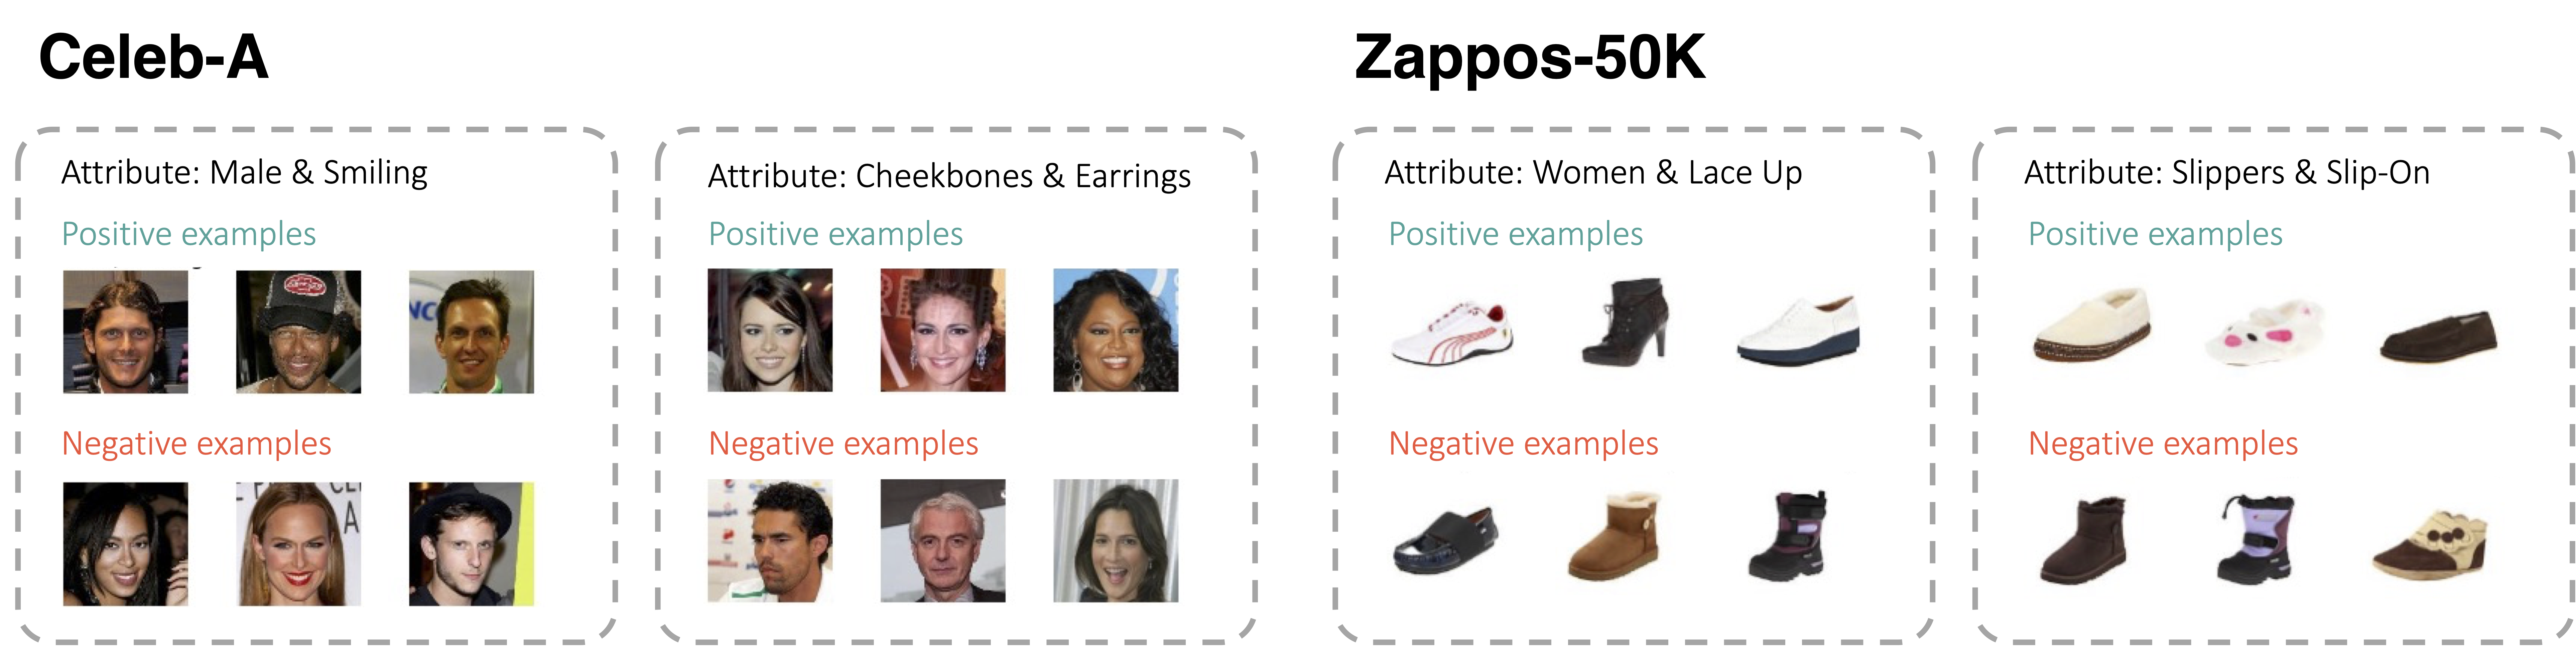
\includegraphics[width=6\linewidth,trim={0 0 0 0},clip]{figures/benchmark-v2.png}
\else
\centering
\savespacefig
\savespacefig
\savespacefig
\savespacefig
\savespacefig
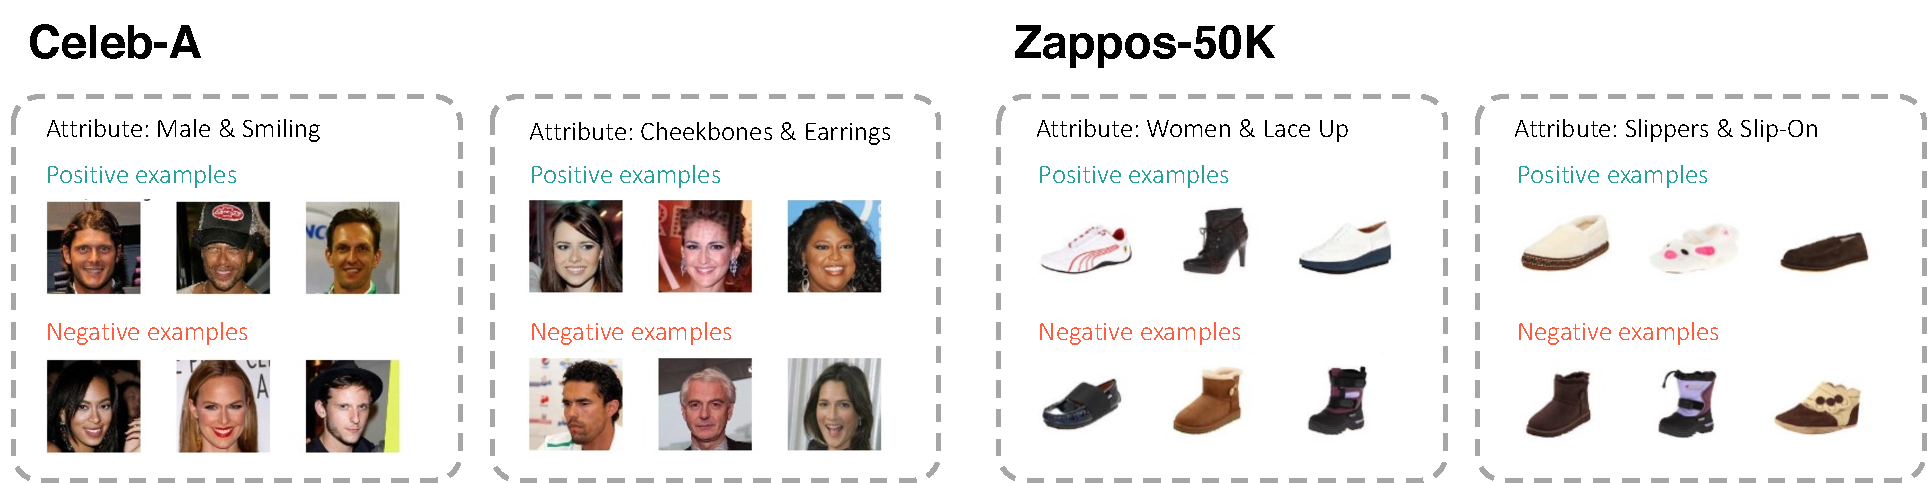
\includegraphics[width=0.97\linewidth,trim={0 0 0 0},clip]{figures/benchmark-v2.pdf}
\fi
\savespacebeforesection
\caption{\textbf{Sample \taskname{} episodes using Celeb-A (left) and Zappos-50K (right).}
Positive and negative examples are sampled according to attributes.}
\label{fig:sample}
\savespacebeforesection
\end{figure*}

% !TEX root = ../main.tex

\section{Online Contextualized Few-Shot Learning}
\vspace{-0.1in}
\label{sec:benchmark}
In this section, we introduce our new online contextualized few-shot learning (OC-FSL) setup in the
form of a sequential decision problem, and then introduce our new benchmark datasets.

\vspace{-0.1in}
\paragraph{Continual few-shot classification as a sequential decision problem:}
In traditional few-shot learning, an episode is constructed by a support set $S$ and a query set
$Q$. A few-shot learner $f$ is expected to predict the class of each example in the query set
$\bx^Q$ based on the support set information: $\hat{y}^Q = f(\bx^Q; (\bx^S_1, y^S_1), \dots,
(\bx^S_N, y^S_N))$, where $\bx \in \mathbb{R}^D$, and $y \in [1 \dots K]$. This setup is not a natural fit for continual learning, since it is unclear when
to insert a query set into the sequence.

Inspired by the online learning literature, we can convert continual few-shot learning into a
sequential decision problem, where every input example is also part of the evaluation: $\hat{y}_t =
f(\bx_t; (\bx_1, \tilde{y}_1), \dots, (\bx_{t-1}, \tilde{y}_{t-1}))$, for $t = 1 \dots T$, where
$\tilde{y}$ here further allows that the sequence of inputs to be semi-supervised: $\tilde{y}$
equals $y_t$ if labeled, or otherwise $-1$. The setup in \citet{mann} and \citet{rareevent} is
similar; they train RNNs using such a temporal sequence as input. However, their evaluation relies
on a ``query set'' at the end. We instead evaluate online while learning.

Figure~\ref{fig:setup}-A illustrates these features, using an example of an input sequence where an
agent is learning about new objects in a kitchen. The model is rewarded when it correctly predicts a
known class or when it indicates that the item has yet to be assigned a label.

\vspace{-0.1in}
\paragraph{Contextualized environments:}
Typical continual learning consists of a sequence of tasks, and models are trained sequentially for
each task. This feature is also preserved in many incremental learning settings~\citep{icarl}. For
instance, the split-CIFAR task divides CIFAR-100 into 10 learning environments, each with 10
classes, presented sequentially. In our formulation, the sequence returns to earlier environments
(see Figure~\ref{fig:setup}-B), which enables assessment of long-term durability of knowledge.
Although the ground-truth environment identity is not provided, we structure the task such that the
environment itself provides contextual cues which can constrain the correct class label.
\emph{Spatial} cues in the input help distinguish one environment from another. \emph{Temporal} cues
are implicit because the sequence tends to switch environments infrequently, allowing recent inputs
to be beneficial in guiding the interpretation of the current input.

\begin{figure}[t]
\centering
\vspace{-0.5in}
\iflatexml
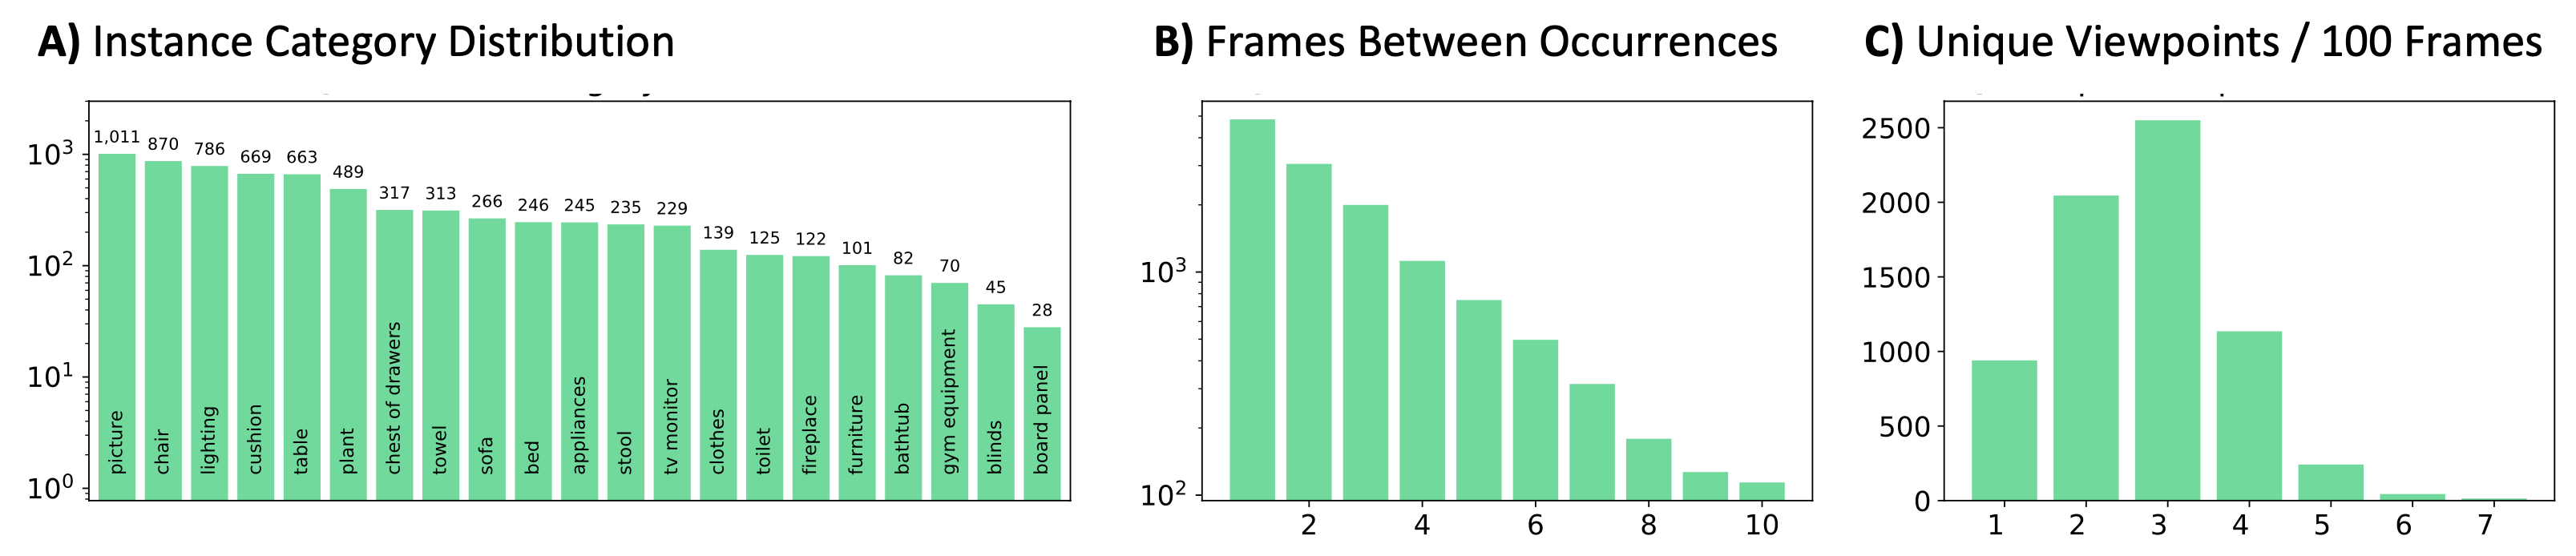
\includegraphics[width=6\textwidth]{figures/condensedv2.png}
\else
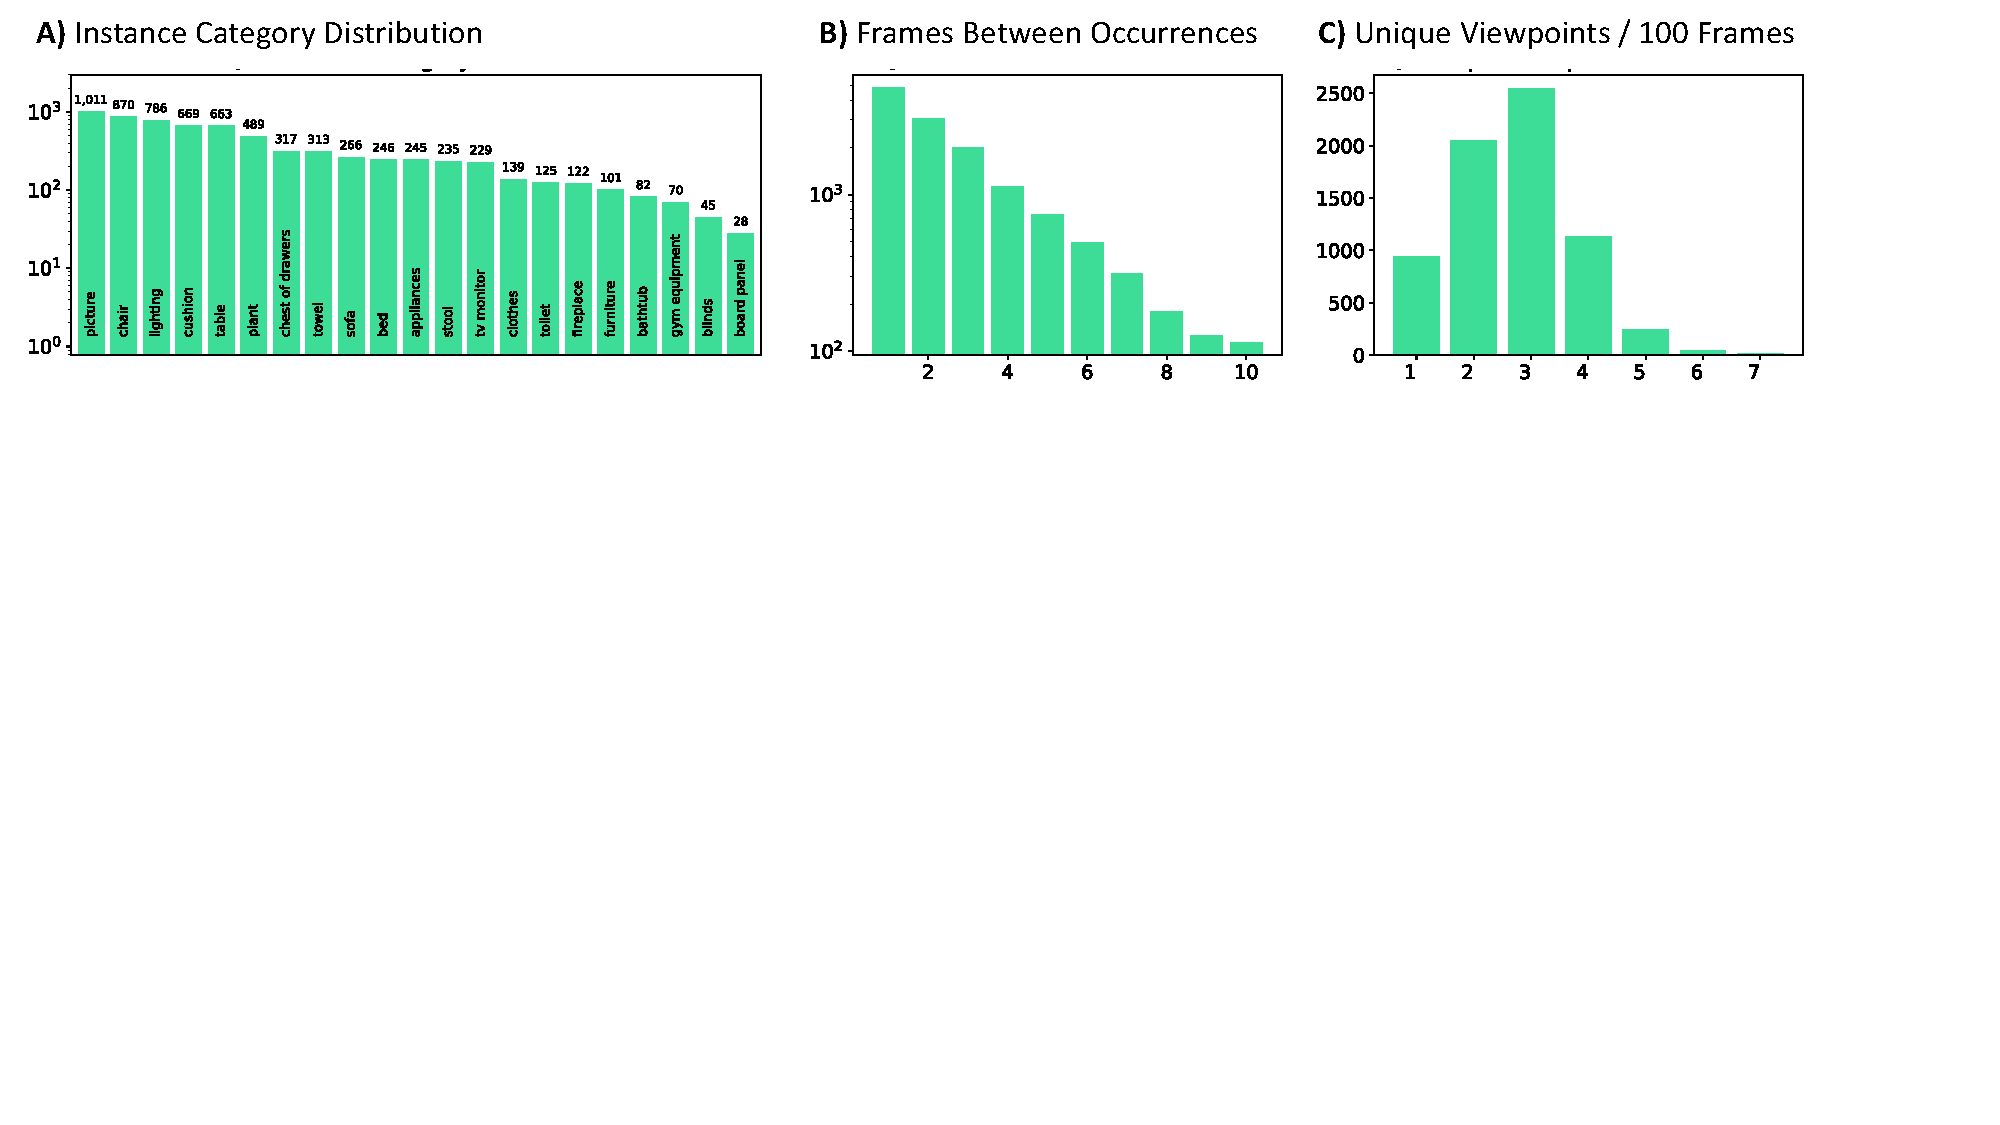
\includegraphics[width=\textwidth,trim={0cm 12.5cm 2.5cm 0cm},clip]{figures/condensedv2.pdf}
\fi
\vspace{-.25in}
\caption{\textbf{Statistics for our \ourroom{} dataset.}
Plots show a natural long tail distribution of instances grouped into categories. An
average sequence has 3 different view points. Sequences are highly correlated in time but revisits
are not uncommon. }
\label{fig:dataset_distribution}
\vspace{-0.15in}
\end{figure}

\vspace{-0.1in}
\paragraph{\ourchar{}:}
The Omniglot dataset~\citep{omniglot} contains 1623 handwritten characters from 50 different
alphabets. We split the alphabets into 31 for training, 5 for validation, and 13 for testing. We
augment classes by 90 degree rotations to create 6492 classes in total. Each contextualized few-shot
learning image sequence contains 150 images, drawn from a random sample of 5-10 alphabets, for a
total of 50 classes per sequence. These classes are randomly assigned to 5 different environments;
within an environment, the characters are distributed according to a Chinese restaurant
process~\citep{crp} to mimic the imbalanced long-tail distribution of naturally occurring objects. We
switch between environments using a Markov switching process; i.e., at each step there is a constant
probability of switching to another environment. An example sequence is shown in
Figure~\ref{fig:dataset}-A.

\vspace{-0.1in}
\paragraph{\ourroom{}:}
As none of the current few-shot learning datasets provides the natural online learning experience
that we would like to study, we created our own dataset using simulated indoor environments. We
formulate this as a few-shot instance learning problem, which could be a use case for a home robot:
it needs to quickly recognize and differentiate novel object instances, and large viewpoint
variations can make this task challenging (see examples in Figure~\ref{fig:dataset}-B). There are
over 7,000 unique instance classes in the dataset, making it suitable to meta-learning approaches.

Our dataset is derived from the Matterport3D dataset~\citep{matterport} with 90 indoor worlds
captured using panoramic depth cameras. We split these into 60 worlds for training, 10 for
validation and 20 for testing. MatterSim~\citep{mattersim} is used to load the simulated world and
collect camera images and HabitatSim~\citep{habitat} is used to project instance
segmentation labels onto 2D image space. We created a random walking agent to collect the virtual
visual experience. For each viewpoint in the random walk, we randomly sample one object from
the image sensor and highlight it with the available instance segmentation, forming an input {\it
frame}. Each viewpoint provides environmental context---the other objects present in the
room with the highlighted object.

Figure~\ref{fig:dataset_distribution}-A shows the object instance distribution. We see strong
temporal correlation, as 30\% of the time the same instance appears in the next frame
(Figure~\ref{fig:dataset_distribution}-B), but there is also a significant proportion of revisits.
On average, there are three different viewpoints per 100-image sequence
(Figure~\ref{fig:dataset_distribution}-C). Details and other statistics of our proposed datasets are
included in the Appendix.

\vspace{-0.1in}
\paragraph{\ourimg{}:} To make the classification problem more challenging, we also report results 
on \ourimg, which uses the same online sequence sampler as \ourchar{} but applied on the \textit{tiered}-ImageNet 
dataset~\citep{fewshotssl}, a subset of the original ImageNet dataset~\citep{imagenet}.
It contains 608 classes with a total of 779K images of size 84$\times$84.
We use the same split of classes as \citet{fewshotssl}. The high-level categories are used for
sampling different ``environments'' just like the notion of alphabets in \ourchar{}.

% !TEX root = ../arxiv.tex

\savespacebeforesection
\section{Experiment Methodology}
\savespacebeforesection
\label{sec:method}

In this section, we describe a range of methods that can be used for the
problem of
\titlelower{}. The methods can be organized into two stages. The first stage is
representation learning through either pre-training the network or performing
meta-learning. The second stage is learning a few-shot classifier at test-time
to solve a new episode. We describe each stage of learning below.

\savespacebeforesection
\subsection{Stage I: Representation Learning}
\label{sec:ft}
\savespacebeforesection
We consider the following representation approaches in our evaluation.
\savespacebeforesection
\paragraph{Supervised:} Many of the existing few-shot learning approaches
include a stage of supervised representation learning. Two classes of
approaches are frequently employed:
\iflatexml
\begin{itemize}
\else
\begin{itemize}[leftmargin=*]
\fi
\savespacebeforesection
\item Episodic meta-learning approaches train directly from a set of few-shot
episodes using episodic labels. This class of methods can be naturally applied
to our learning setting.
\item Supervised classification approaches train a network to directly classify
a set of training classes using absolute labels, and at test time, the
embedding network is transferred to solve the test task by training another
classifier on top. If absolute attributes are provided to the learner, then one
natural approach is to instead train an attribute classifier with multiple
binary outputs. After the attribute classifier network is learned, we can then
transfer the representations to recognize test attributes. We denote this
method as Supervised Attributes (\textbf{SA}).
\end{itemize}
\savespacebeforesection
\paragraph{Unsupervised:} 
As supervised representation learning may not generalize to novel attributes,
we also consider unsupervised representation learning as another option. We
chose SimCLR~\citep{simclr} as a representative from this category due to its
empirical success. In general, contrastive learning approaches aim to build
invariant representations between a pair of inputs $\{\mathbf{x},
\mathbf{x'}\}$ that are produced by applying random data augmentations (e.g.
cropping) to an input image. It is likely to preserve more general semantic
features since all attributes are useful towards identifying another random
crop of the same image. We first obtain the embedding output $\mathbf{h}$ from
the CNN, and then following \citep{simclr}, we project $\mathbf{h}$ to
$\mathbf{z}$ using a multi-layered perceptron (MLP): $\mathbf{h} =
\mathrm{CNN}(\mathbf{x}), \mathbf{z} =
\mathrm{MLP}_1(\mathbf{h})$. With a batch of image pairs denoted by
$\{\mathbf{x}_i\}, \{ \mathbf{x}_i'\}$, we can obtain their features
$\{\mathbf{z}_i\}, \{ \mathbf{z}_i'\}$, and the contrastive loss function is
defined similar to the cross entropy function:
\ifarxiv
\begin{align}
    \mathcal{L}_1 = -\sum_i \log\frac{\exp(\mathbf{z}_i \cdot \mathbf{z}_i' /
    \tau)}{\sum_j
    \exp(\mathbf{z}_i \cdot \mathbf{z}_j' / \tau)},
\end{align}
\savespaceeqn
\else
$
    \mathcal{L}_1 = -\sum_i \log\frac{\exp(\mathbf{z}_i \cdot \mathbf{z}_i' /
    \tau)}{\sum_j
    \exp(\mathbf{z}_i \cdot \mathbf{z}_j' / \tau)},
$
\fi
where $\tau$ is a temperature parameter. We denote Unsupervised representation
learning as \textbf{U}.

\savespacebeforesection
\paragraph{Unsupervised-then-Finetuning:} For unsupervised learning, we also
consider adding a subsequent stage of supervised fine-tuning to utilize
attribute labels from the training set. Note that fine-tuning here is different
from fine-tuning in regular few-shot learning as it is not fine-tuning on test
episodes but rather on the original training set. To prevent overwriting the
representations and making them overly sensitive to training attributes, we add
another projection MLP that learns more specific representations for finetuning
on training attributes: $\mathbf{g} = \mathrm{MLP}_2(\mathbf{h}).$ Here, we
again consider using two different modes of supervision: 1) the \taskname{}
binary episodic labels, or 2) the underlying absolute attribute labels:
\iflatexml
\begin{itemize}[leftmargin=*]
\else
\begin{itemize}
\fi
\savespacebeforesection
\item Unsupervised-then-FineTune-on-Episodes (\textbf{\uftpn}).
We adopt the
Prototypical Networks~\citep{protonet} formulation, where the network solves a
learning episode of $N$ positive and negative support examples by using
prototypes $\mathbf{p}$: $\mathbf{p}^+ = \frac{1}{N} \sum_i \mathbf{g}^+_i;
\mathbf{p}^- =
\frac{1}{N} \sum_i \mathbf{g}^-_i.$ With query example $\mathbf{g}^q$, we can
make a binary prediction:
$\hat{y}^q = \frac{\exp(-d(\mathbf{g}^q,
    \mathbf{p}^+))}{\exp(-d(\mathbf{g}^q, \mathbf{p}^+)) +
    \exp(-d(\mathbf{g}^q, \mathbf{p}^-))},$
%\end{align}
% \vskip -0.2cm
where $d$ is some dissimilarity score, \eg Euclidean distance or cosine
dissimilarity, and the training objective is to minimize the classification
loss between the prediction $\hat{y}^q$ and the label $y^q$:
\ifarxiv
\begin{align}
\mathcal{L}_{2E} &= \sum_j - y_j \log \hat{y}^q_j - (1-y^q_j) \log (1 -
\hat{y}^q_j),
\end{align}
where $j$ is the index of query examples.
\else
$\mathcal{L}_{2E} = \sum_j - y_j \log \hat{y}^q_j - (1-y^q_j) \log (1 -
\hat{y}^q_j),$
where $j$ is the index of query examples.
\fi
    
\item Unsupervised-then-FineTune-on-Attributes (\textbf{\uftsa}). With
persistent attribute information, we can train a linear classifier with sigmoid
activation to directly predict the absolute attribute labels $\mathbf{a}$:
$\hat{\mathbf{a}} = W_A \mathbf{g} + b_A$, with the loss being
\ifarxiv
\begin{align}
\mathcal{L}_{2A} &= \sum_k - \mathbf{a}_k \log \hat{\mathbf{a}}_k -
(1-\mathbf{a}_k) \log (1 -
\hat{\mathbf{a}}_k),
\end{align}
\savespaceeqn
\vskip -0.6cm
where $k$ is the index of attributes.
\else
$\mathcal{L}_{2A} = \sum_k - \mathbf{a}_k \log \hat{\mathbf{a}}_k -
(1-\mathbf{a}_k) \log (1 -
\hat{\mathbf{a}}_k),$
where $k$ is the index of attributes.
\fi
\end{itemize}

\savespacebeforesection
\subsection{Stage II: Few-Shot Learning}
\label{sec:fsl}
\savespacebeforesection

Once representations are learned, it remains to be decided how to use the small
support set of each given test episode in order to make predictions for the
associated query set. For each model described in the previous stages, we
consider three candidate approaches: nearest neighbor (\textbf{NN}) used in
MatchingNet~\citep{matchingnet}, the nearest centroid (\textbf{NC}) used in
ProtoNet~\citep{protonet}, and logistic regression (\textbf{LR}) used in
\citet{closerlook}. The LR approach learns a weight coefficient for each
feature dimension, thus performing some level of feature selection, unlike the
NC or NN alternatives. In addition, we apply an L1 regularizer on LR to
encourage sparsity. In this way, the learning of a classifier is essentially
done at the same time as the selection of feature dimensions. The overall
objective of the classifier is:
\ifarxiv
\begin{align}
\argmin_{\mathbf{w}, b} - y \log(\hat{y}) - (1-y) \log(1 - \hat{y}) + 
\lambda \lVert \mathbf{w}
\rVert_1,
\end{align}
\else
$
\argmin_{\mathbf{w}, b} - y \log(\hat{y}) - (1-y) \log(1 - \hat{y}) + 
\lambda \lVert \mathbf{w}
\rVert_1,$
\fi
where $\hat{y} = \sigmoid(\mathbf{w}^\top \mathbf{h} + b)$, and $\mathbf{h}$ is
the representation vector extracted from the CNN backbone. Note that in this
stage we discard the projection MLPs that are defined in previous stages since
they are trained towards training attributes and self-supervised objectives,
and we found that they do not transfer well to novel attributes.

% !TEX root = ../arxiv.tex
\begin{table*}
\iflatexml
    \begin{tabular}{cll}
    \toprule
    \bf Paradigm                  & \bf Test time task                                   & \bf Task specification     \\
    \hline                                                                                                                  ZSL~\citep{attributezsl}      & Novel semantic classes of existing attributes        & Attribute IDs         \\
    CZSL~\citep{czsl}             & Novel combinations of existing attributes \& classes & Attribute IDs \\
    FSL~\citep{lake2011oneshot}   & Novel semantic classes                        & Support examples           \\   
    \midrule
    \taskname{} (Ours)             & Novel (previously unlabeled) attributes      & Support examples           \\
    \bottomrule
    \end{tabular}
\else
    \savespacefig
    \savespacefig
    \savespacefig
    \savespacefig
    \begin{center}
    \begin{small}
    \ifarxiv
    \resizebox{\textwidth}{!}{
    \begin{tabular}{cll}
    \toprule
    \bf Paradigm                  & \bf Test time task                                   & \bf Task specification     \\
    \hline                                                                                                                  ZSL~\citep{attributezsl}      & Novel semantic classes of existing attributes        & Attribute IDs         \\
    CZSL~\citep{czsl}             & Novel combinations of existing attributes \& classes & Attribute IDs \\
    FSL~\citep{lake2011oneshot}   & Novel semantic classes                        & Support examples           \\   
    \midrule
    \taskname{} (Ours)             & Novel (previously unlabeled) attributes      & Support examples           \\
    \bottomrule
    \end{tabular}
    }
    \else
    \resizebox{0.8\textwidth}{!}{
    \begin{tabular}{cll}
    \toprule
    \bf Paradigm                  & \bf Test time task                                   & \bf Task specification     \\
    \hline                       
    ZSL~\citep{attributezsl}      & Novel semantic classes of existing attributes        & Attribute IDs         \\
    CZSL~\citep{czsl}             & Novel combinations of existing attributes \& classes & Attribute IDs \\
    FSL~\citep{lake2011oneshot}   & Novel semantic classes                        & Support examples           \\   
    \midrule
    \taskname{} (Ours)             & Novel (previously unlabeled) attributes      & Support examples           \\
    \bottomrule
    \end{tabular}
    }
    \fi
    \end{small}
    \end{center}
    \savespacebeforesection
\fi
\caption{\textbf{Differences between  zero-shot learning (ZSL), compositional ZSL (CZSL), few-shot
learning (FSL), and our newly proposed \titlelower{} (\taskname{}).} Our task requires the model to
generalize to new attributes.}
\label{tab:benchmarkdiff}
\savespacebeforesection
\end{table*}

% !TEX root = ../arxiv.tex
\savespacebeforesection
\section{Related Work}
\savespacebeforesection
\paragraph{Few-shot learning:}
Few-shot learning (FSL)~\citep{fei2006one,lake2011oneshot,matchingnet} entails
learning new tasks with only a few examples. With an abundance of training
data, FSL is closely related to the general meta-learning or learning to learn
paradigm~\citep {Thrun1998}, as a few-shot learning algorithm can be developed
on training tasks and run on novel tasks at test time. In standard few-shot
classification, each image only has a single unambiguous class label, whereas
in our few-shot attribute learning, the target attributes can vary depending on
how the support set is presented. We show in this paper that this is a more
challenging problem as it requires the model to be more flexible and
generalizable. In early benchmarks, a set of semantic classes was randomly
split into a training and test set. We hypothesize that this often leads to a
common set of attributes that span (most of) the training and test classes,
thus causing high transferability between these two sets, which allows simple
solutions based on feature re-use \citep{closerlook,anil} to work well. Later
benchmarks explicitly attempt to vary the separation between train and test
classes, based on varying the distances in the underlying WordNet classes
(\textit{tiered}-ImageNet \citep{fewshotssl}), or in different image domains
(Meta-Dataset \citep{triantafillou2019meta}). However, we argue that reasoning
about the underlying attributes directly offers a more systematic framework to
measure the relatedness and transferability between the train and test set. We
expect our analysis to open the door to such studies in the future. Few-shot
attribute learning is also related to multi-label few-shot
learning~\citep{alfassy2019laso,li2021compositional} and compositional few-shot learning~\citep{tokmakov2019learning}. These prior works
emphasize on the compositional aspect, whereas we propose models that address
the transferability of the learned representations.
Additionally,
\citet{xiang2019incremental} explored combining incremental few-shot learning
and attribute learning for pedestrian images.

\savespacebeforesection
\paragraph{Attribute learning:}
In the past, there have been a number of works that aim to predict attribute
information from raw
inputs~\citep{ferrari2007attribute,farhadi2009describe,farhadi2010attribute,wang2010discriminative}.
A related model is later proposed by \citet{koh2020concept} to achieve better
causal interpretability.% \citet{escorcia2015relationship} found that certain
% hidden units of a deep neural network predicts attributes very well. 
There have also been a number of datasets that have been collected with visual
attributes annotated
\citep{cub,zappos,celeba,patterson2016coco,pham2021attribute}. One key
difference between our work and these attribute learning approaches is that at
test time we aim to learn a classifier on novel attributes that are previously
not labeled in the training set, and this brings additional challenges of
transfer learning and learning with limited labeled data.

\savespacebeforesection
\paragraph{Zero-shot learning:} In zero-shot learning
(ZSL)~\citep{farhadi2009describe,labelembed,goodbadugly,attributezsl,ezzsl,evaluateoutput},
a model is asked to recognize classes not present in the training set,
supervised only by some auxiliary description~\citep{descriptionzsl} or
attribute values~\citep{farhadi2009describe} (see~\citet{wang2019survey} for a
survey). \citet{attributezsl} studied the \textit{direct attribute prediction}
method, similar to the Supervised Attribute baseline described in
Section~\ref{sec:baselines}. Compositional ZSL aims at learning
classes~\citep{czsl,taskdriven,taskaware,unseencomposition} defined by a novel
composition of labeled attributes and object classes. An important distinction
between ZSL and our few-shot attribute learning task is that ZSL uses the same
set of attributes for both training and testing; by contrast, our task asks the
model to learn attributes for which there are no labels during training, and
they may not be relevant to any of the training attributes or episodes. We
summarize the relationships between ZSL, FSL and our task in
Table~\ref{tab:benchmarkdiff}.

% \savespacebeforesection
% \paragraph{Context dependent similarity:} Unlike standard few-shot learning, in
% our learning episodes, the context information is essential for discovering the
% relevant attribute shared among the set of positive examples. The idea of
% context dependent similarity of features explored in the present work takes one
% step towards a more human-like decision maker. As an example provided by
% \citet{tversky1977features}, Cuba is similar to Jamaica in terms of geographic
% proximity, but similar to (Soviet) Russia when speaking of political
% viewpoints. Conditional similarity networks~\citep{condsimnet} proposed
% learning a feature mask for different pre-defined contexts such as colors or
% styles, using the triplet objective~\citep{finegrainsim}. Similarly,
% \citet{contextvissim} proposed to learn a different linear matrix for each
% context. In this paper, we study learning \textit{novel} contextual
% similarities in the form of attributes using only a few training examples.

\savespacebeforesection
\paragraph{Generalization to novel tasks:}
\looseness=-1 
One key component of our work is an attempt to understand the generalization
behavior of learning novel concepts at test time. Relevant theoretical studies
consider novel task generalization, casting it in a transfer learning and
learning to learn
framework~\citep{baxter2000model,ben2008notion,ben2010theory,pentina2014,amit2018meta,lucas2020lb}.
A common theme in these studies is in characterizing task relatedness, and the
role that it plays in generalization to novel tasks.
\citet{arnold2021embedding} studied task clustering for few-shot learning in
the embedding space and found class splits that are of different difficulty
levels. \citet{sariyildiz2021} use the WordNet hierarchy to compute semantic
distances. In our paper, we instead split the data in the attribute space, and
if we assume that semantic classes are combinations of attributes, then a
disjoint attribute split will imply further semantic distances.  In our work,
we investigate the role of task relatedness empirically by investigating
generalization performance under different splits of the attribute space.
% !TEX root = ../main.tex
\section{Experiments}
\vspace{-0.1in}
In this section, we show experimental results for our online contextualized few-shot learning
paradigm, using \ourchar{} and \ourroom{} (see Sec.~\ref{sec:benchmark}) to evaluate our model, CPM,
and other state-of-the-art methods. For Omniglot, we apply an 8$\times$8 CutOut~\citep{cutout} to
each image to make the task more challenging. 
% Details about the split information can be found in
% Appendix~\ref{app:data}.

\vspace{-0.1in} \paragraph{Implementation details:} For \ourchar{}, we use the common
4-layer CNN for few-shot learning with 64 channels in each layer. For \ourimg{}, we also use ResNet-12 
with input resolution 84$\times$84~\citep{tadam}. For the \ourroom{}, we resize the input to 
120$\times$160 and use ResNet-12. To represent
the feature of the input image with an attention mask, we concatenate the global average pooled
feature with the attention ROI feature, resulting in a 512d feature vector. For the contextual RNN,
in both experiments we used an LSTM~\citep{lstm} with a 256d hidden state. The best CPM model is
equipped using GAU and cosine similarity for querying prototypes. Logits based on cosine similarity
are multiplied with a learned scalar initialized at 10.0~\citep{tadam}. We include additional
training details in Appendix~\ref{app:exp}.

\vspace{-0.1in}
\paragraph{Evaluation metrics:}
In order to compute a single number that characterizes the learning ability over sequences, we
propose to use \textit{average precision} (AP) to evaluate
both with respect to old versus new and the
specific class predictions.
Concretely, all predictions are sorted by their old vs. new scores, and we compute AP using the area
under the precision-recall curve. A true positive is defined as the correct prediction of a
multi-class classification among known classes. We also compute the ``$N$-shot'' accuracy; i.e., the
average accuracy after seeing the label $N$ times in the sequence. Note that these accuracy scores
only reflect the performance on {\it known} class predictions. All numbers are reported with an
average over 2,000 sequences and for $N$-shot accuracy standard error is also included.
Further explanation of these metrics is in Appendix~\ref{sec:metrics}. 

\vspace{-0.1in}
\paragraph{Comparisons:}
To evaluate the merits of our proposed model, we implement classic few-shot learning and online
meta-learning methods. More implementation and training details of these baseline methods can be
found in Appendix~\ref{app:exp}.
% !TEX root = ../main.tex
\begin{figure}[t]
\vspace{-0.5in}
\centering
\iflatexml
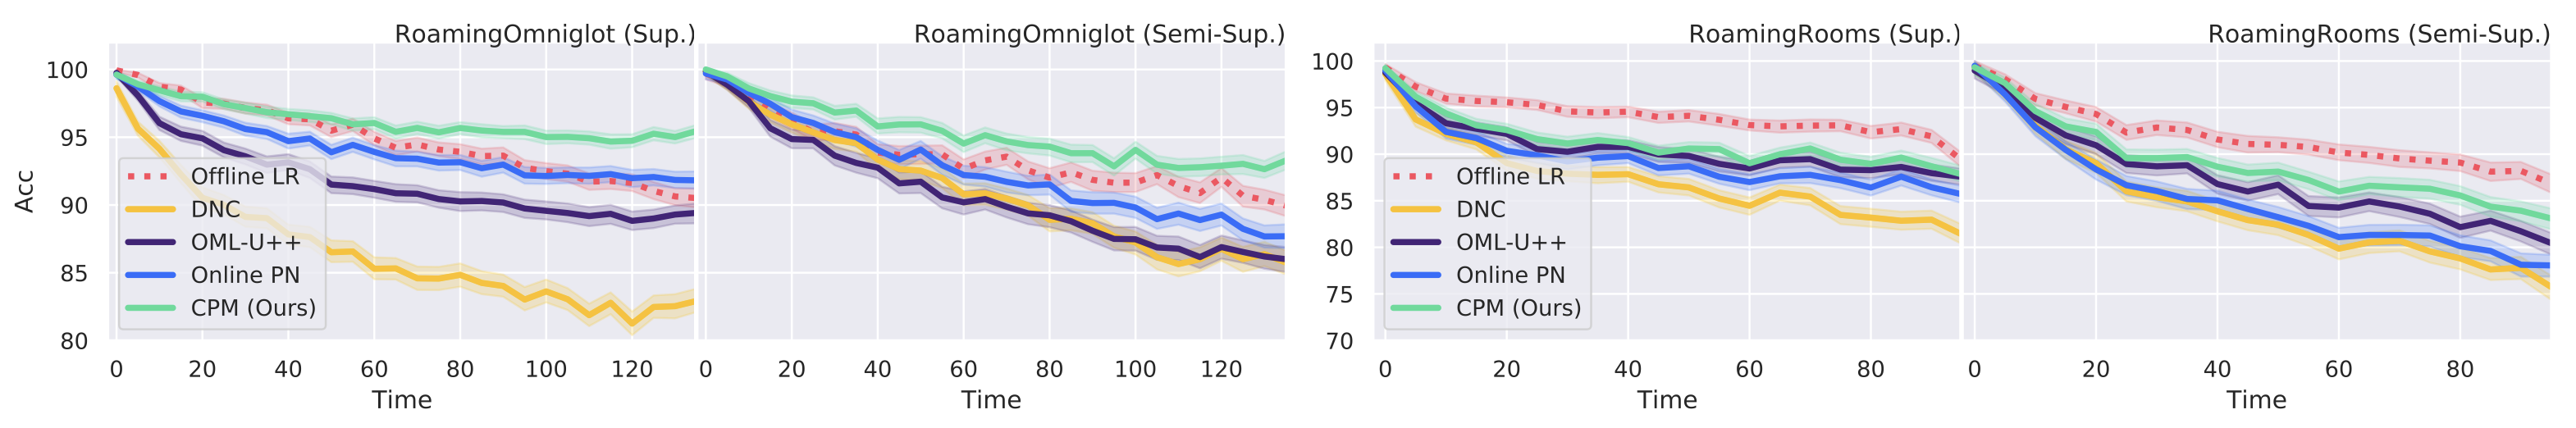
\includegraphics[width=6\linewidth]{figures/acctime_full.png}
\else
\setlength{\tabcolsep}{0pt}
\begin{tabular}{cccc}
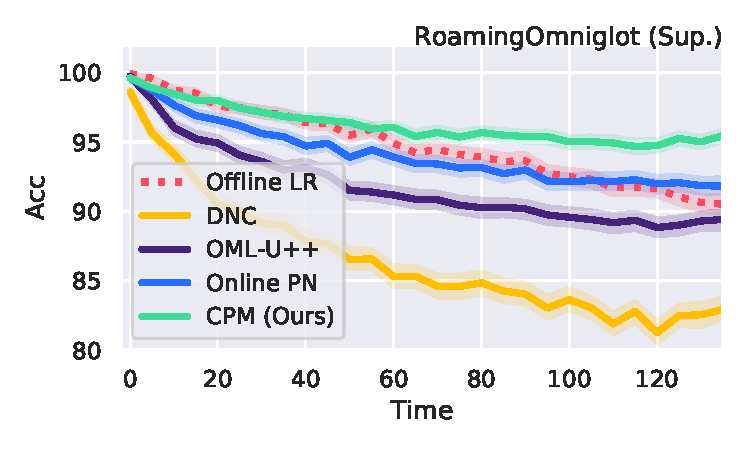
\includegraphics[height=2.4cm,trim={0.3cm 0cm 0.5cm 0},clip]{figures/omniglot-nossl-time.pdf}
&
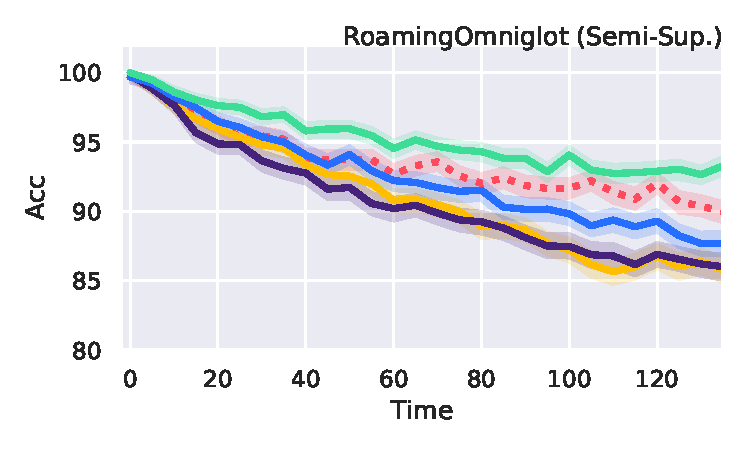
\includegraphics[height=2.4cm,trim={2cm 0cm 0cm 0},clip]{figures/omniglot-ssl-time.pdf}
&
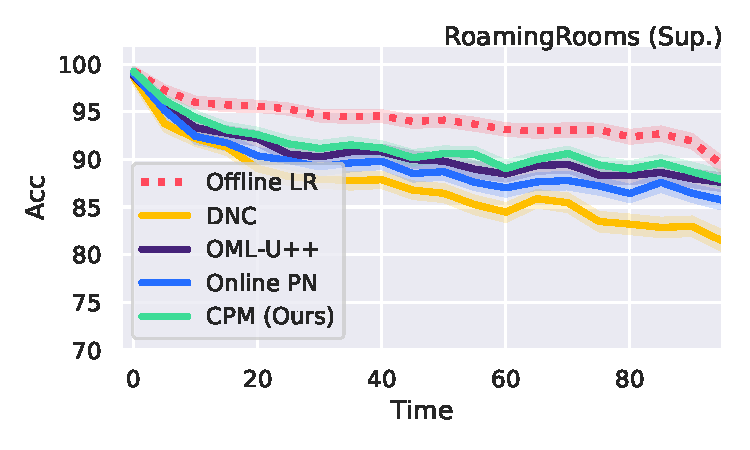
\includegraphics[height=2.4cm,trim={1cm 0cm 0.5cm 0},clip]{figures/matterport-nossl-time.pdf}
&
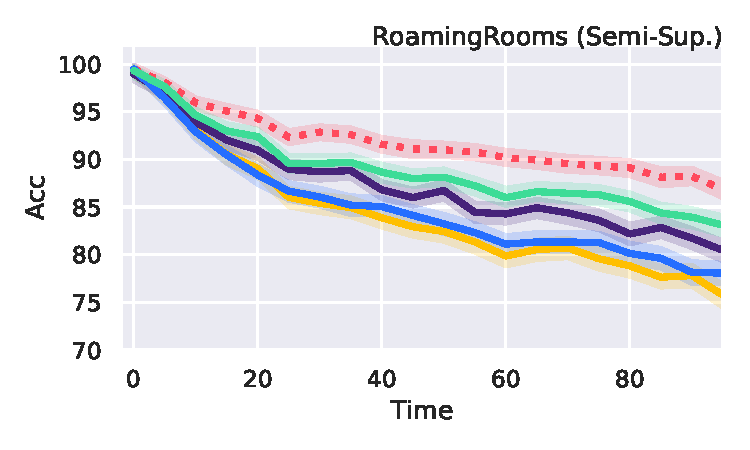
\includegraphics[height=2.4cm,trim={2cm 0cm 0cm 0},clip]{figures/matterport-ssl-time.pdf}
\\
\end{tabular}
\vspace{-0.25in}
\fi
\caption{\textbf{Few-shot classification accuracy over time.} \textbf{Left:} \ourchar{}.
\textbf{Right:} \ourroom{}. \textbf{Top:} Supervised. \textbf{Bottom:} Semi-supervised. An offline
logistic regression (Offline LR) baseline is also included, using pretrained ProtoNet features. It
is trained on all labeled examples except for the one at the current time step.}
\label{fig:acctimefull}
% \vspace{-0.25in}
\end{figure}

% !TEX root = ../main.tex
\begin{figure}[t]
\vspace{-0.1in}
\centering
\iflatexml
    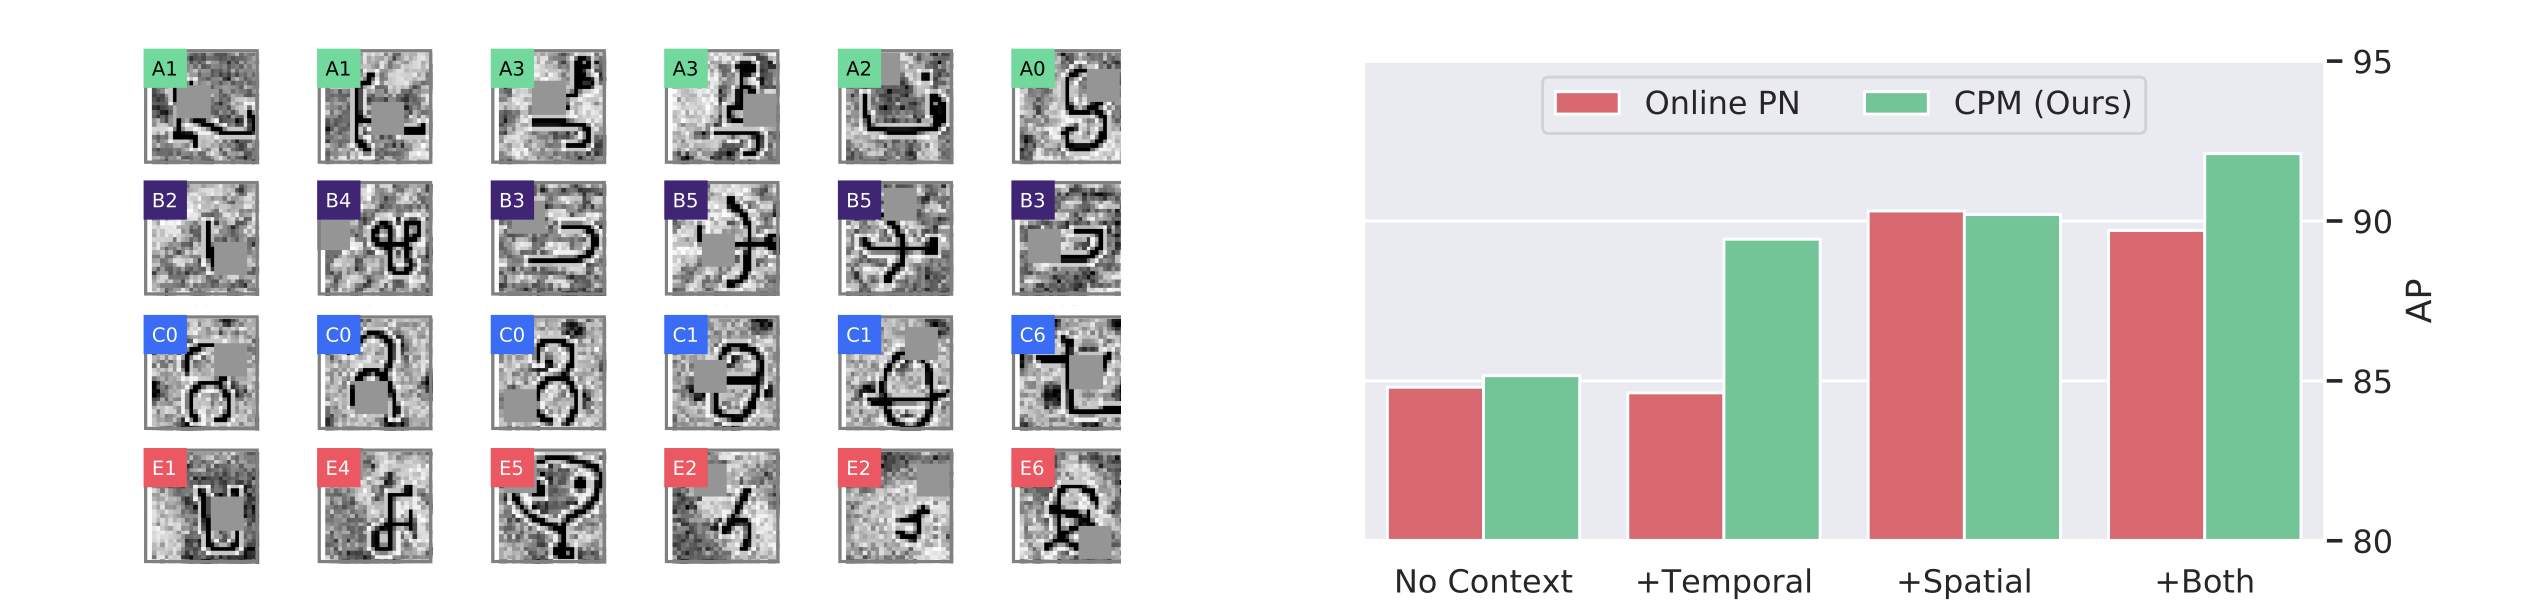
\includegraphics[width=6\linewidth]{figures/spatiotemporal_full.png}
\else
    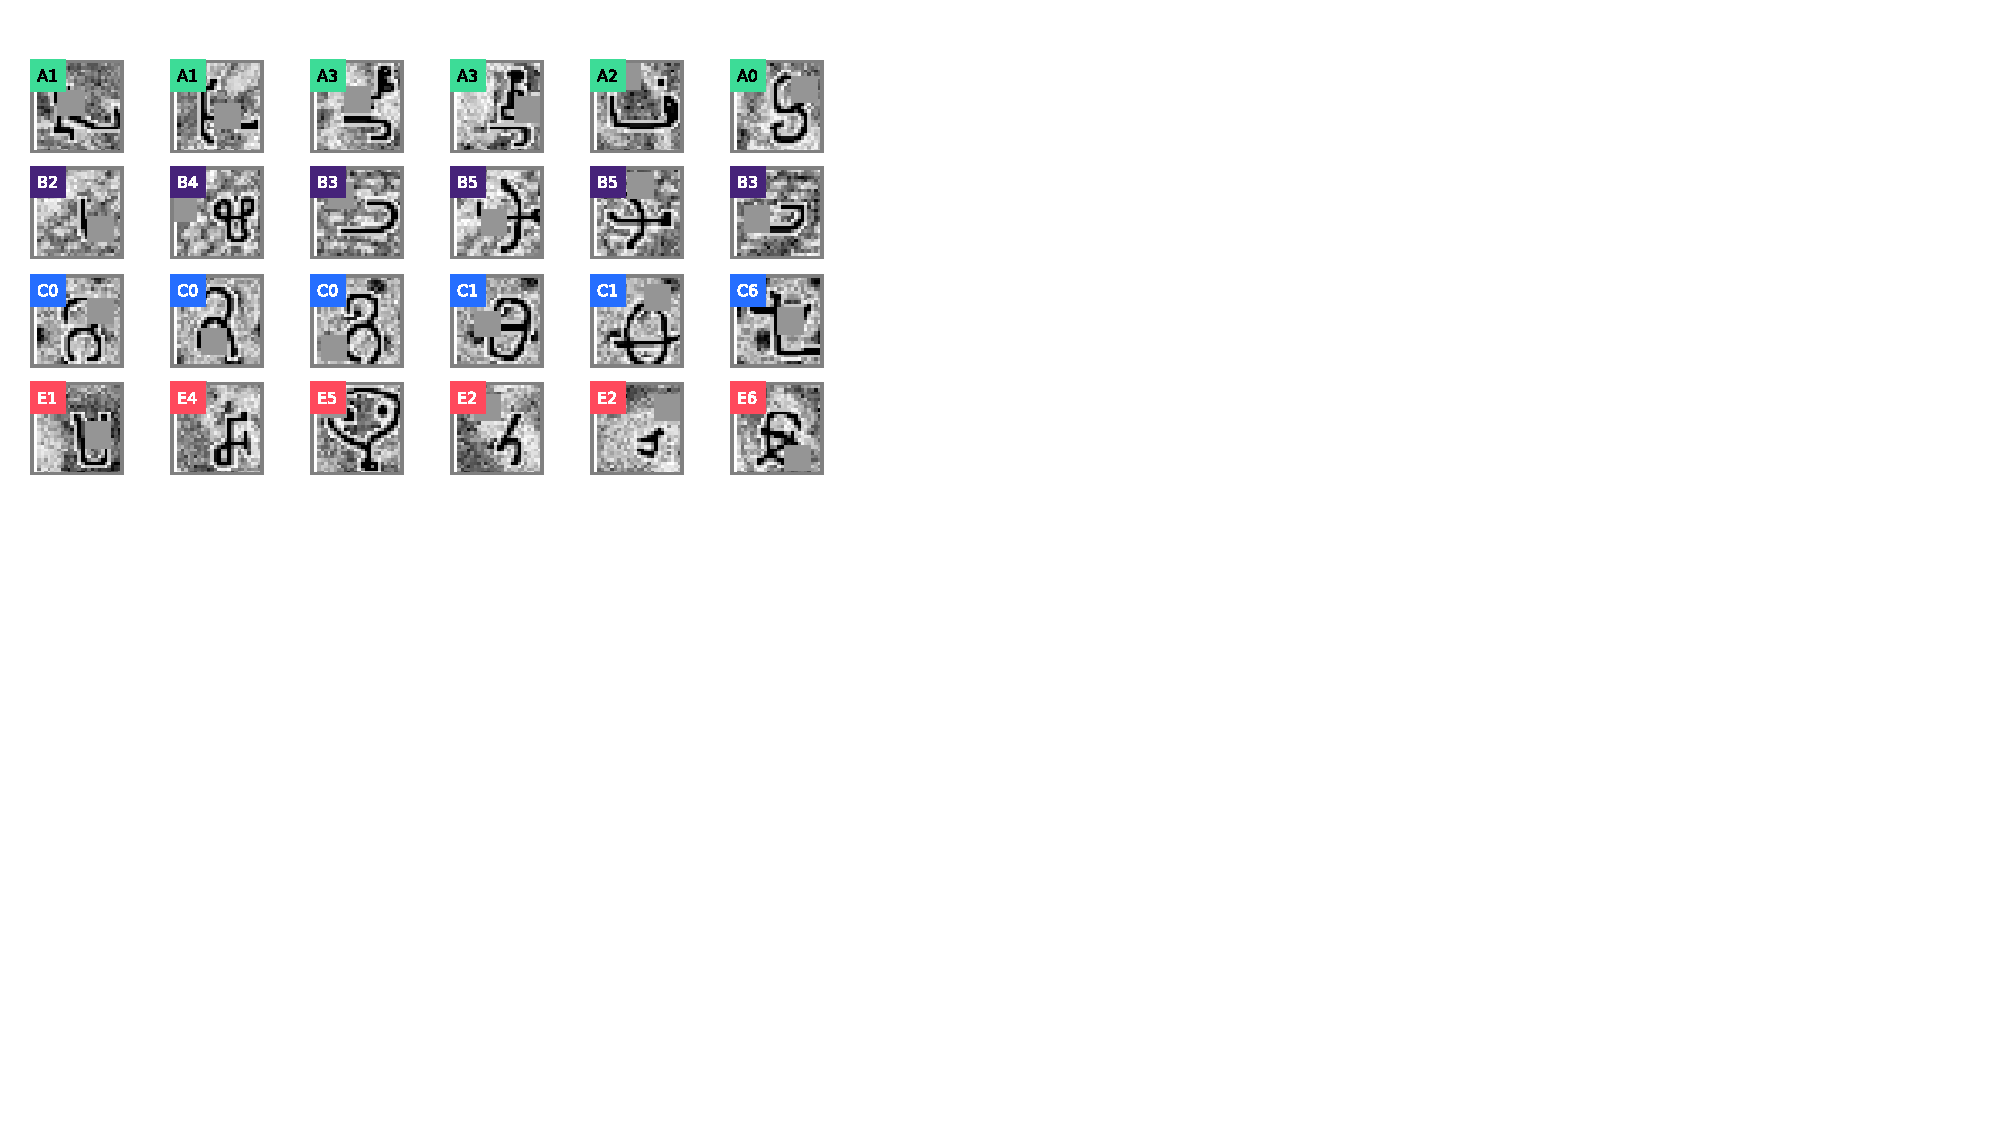
\includegraphics[height=2.8cm,trim={-2.25cm 10cm 20cm 0.5cm},clip]{figures/omniglot-texture.pdf}
    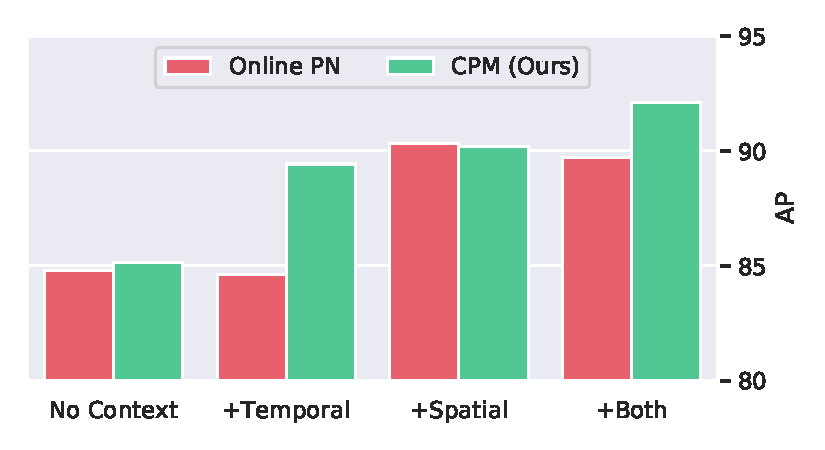
\includegraphics[height=2.8cm,trim={-2.25cm 0 0.5cm 0},clip]{figures/spatiotemporal.pdf}
\fi
\quad
\vspace{-0.2in}
\caption{\textbf{Effect of spatiotemporal context.} Spatiotemporal
context are added separately and together in \ourchar{}, by introducing texture background and
temporal correlation. \textbf{Left:} Stimuli used for spatial cue of the background environment.
\textbf{Right:} Our CPM model benefits from the presence of a temporal context
(``+Temporal'' and ``+Both'')} %, while Spatial context helps both CPM and online ProtoNet.}
\label{fig:spatiotemporal}
% \vspace{-0.1in}
\end{figure}

\vspace{-0.1in}
\iflatexml
\begin{itemize}
    \item \textbf{OML}~\citep{oml}: This is an online version of MAML~\citep{maml}. It performs one
    gradient descent step for each labeled input image, and slow weights are learned via
    backpropagation through time. On top of OML, we added an unknown predictor $\hat{u}_t = 1 -
    \max_k \hat{y}_{t,k}$ \footnote{We tried a few other ways and this is found to be the
    best.} (\textbf{OML-U}). We also found that using cosine classifier without the last layer ReLU
    is usually better than using the original dot-product classifier, and this improvement is denoted
    as \textbf{OML-U++}.
    \item \textbf{LSTM}~\citep{lstm} \& \textbf{DNC}~\citep{dnc}: We include RNN methods for
    comparison as well. Differentiable neural computer (DNC) is an improved version of memory
    augmented neural network (MANN)~\citep{mann}.
    \item \textbf{Online MatchingNet (\OnlineMatchingNet{})}~\citep{matchingnet}, 
    \textbf{IMP (\OnlineIMP{})}~\citep{imp} \&
    \textbf{ProtoNet (\OnlineProtoNet{})}~\citep{protonet}: We used\ the same negative Euclidean distance as the
    similarity function for these three metric learning based approaches.  In particular,
    MatchingNet stores all examples and performs nearest neighbor matching, which can be memory
    inefficient. Note that Online ProtoNet is a variant of our method without the contextual RNN.
\end{itemize}
\else
\begin{itemize}[leftmargin=*]
    \item \textbf{OML}~\citep{oml}: This is an online version of MAML~\citep{maml}. It performs one
    gradient descent step for each labeled input image, and slow weights are learned via
    backpropagation through time. On top of OML, we added an unknown predictor $\hat{u}_t = 1 -
    \max_k \hat{y}_{t,k}$ \footnote{We tried a few other ways and this is found to be the
    best.} (\textbf{OML-U}). We also found that using cosine classifier without the last layer ReLU
    is usually better than using the original dot-product classifier, and this improvement is denoted
    as \textbf{OML-U++}.
    \item \textbf{LSTM}~\citep{lstm} \& \textbf{DNC}~\citep{dnc}: We include RNN methods for
    comparison as well. Differentiable neural computer (DNC) is an improved version of memory
    augmented neural network (MANN)~\citep{mann}.
    \item \textbf{Online MatchingNet (\OnlineMatchingNet{})}~\citep{matchingnet}, 
    \textbf{IMP (\OnlineIMP{})}~\citep{imp} \&
    \textbf{ProtoNet (\OnlineProtoNet{})}~\citep{protonet}: We used\ the same negative Euclidean distance as the
    similarity function for these three metric learning based approaches.  In particular,
    MatchingNet stores all examples and performs nearest neighbor matching, which can be memory
    inefficient. Note that Online ProtoNet is a variant of our method without the contextual RNN.
\end{itemize}
\fi
\iflatexml
\begin{table}[t]
    \centering
    \begin{tabular}{ccccccc|cccccc}
    \toprule
    & \multicolumn{6}{c|}{\textbf{Supervised}} & \multicolumn{6}{c}{\textbf{Semi-Supervised}}\\
    Interval  &   1 - 2&      3 - 5&      6 - 10&     11 - 20&    21 - 50&    51 - 100&
                    1 - 2&      3 - 5&      6 - 10&     11 - 20&    21 - 50&    51 - 100\\
    OPN 1-Shot  &   88.8&       86.9&       85.2&       84.7&	    83.6&	    81.1&
                    90.1&       88.9&	    88.4&	    87.6&	    87.3&	    85.1\\
    CPM 1-Shot  &   \tb{96.1}&  \tb{94.0}&	\tb{93.0}&  \tb{91.6}&	\tb{88.2}&  \tb{84.6}&
                    \tb{95.9}&  \tb{93.8}&  \tb{92.8}&  \tb{91.8}&	\tb{89.4}&  \tb{85.7}\\
    OPN 3-Shot  &   97.2&	    97.1&	    96.6&	    96.7&	    \tb{96.5}&	95.3&
                    97.8&	    97.3&	    97.1&	    \tb{97.8}&	\tb{97.7}&  \tb{96.8}\\
    CPM 3-Shot  &   \tb{98.5}&	\tb{98.2}&	\tb{97.5}&	\tb{97.2}&      95.4&   \tb{95.5}&
                    \tb{98.7}&	\tb{97.5}&	\tb{97.5}&	    96.5&	    96.3&	    92.9\\
    \bottomrule
    \end{tabular}
    \caption{\textbf{Effect of forgetting over a time interval on \ourchar{}.} Average accuracy vs. the number of time steps since the model has last seen the label of a particular class.}
    \label{tab:forgetomniglot}
\end{table}
\else
\begin{table}[t]
\vspace{-0.5in}
    \centering
    \caption{\textbf{Effect of forgetting over a time interval on \ourchar{}.} Average accuracy vs. the number of time steps since the model has last seen the label of a particular class.}
    \vspace{0.1in}
    \resizebox{\textwidth}{!}{
    \begin{tabular}{ccccccc|cccccc}
    \toprule
    & \mc{6}{c}{\bf Supervised} & \mc{6}{c}{\bf Semi-Supervised}\\
    Interval  &   1 - 2&      3 - 5&      6 - 10&     11 - 20&    21 - 50&    51 - 100&
                    1 - 2&      3 - 5&      6 - 10&     11 - 20&    21 - 50&    51 - 100\\
    \midrule
    OPN 1-Shot  &   88.8&       86.9&       85.2&       84.7&	    83.6&	    81.1&
                    90.1&       88.9&	    88.4&	    87.6&	    87.3&	    85.1\\
    CPM 1-Shot  &   \bf{96.1}&  \bf{94.0}&	\bf{93.0}&	\bf{91.6}&	\bf{88.2}&  \bf{84.6}&
                    \bf{95.9}&  \bf{93.8}&  \bf{92.8}&	\bf{91.8}&	\bf{89.4}&	\bf{85.7}\\
    \midrule
    OPN 3-Shot  &   97.2&	    97.1&	    96.6&	    96.7&	    \bf{96.5}&	95.3&
                    97.8&	    97.3&	    97.1&	    \bf{97.8}&	\bf{97.7}&  \bf{96.8}\\
    CPM 3-Shot  &   \bf{98.5}&	\bf{98.2}&	\bf{97.5}&	\bf{97.2}&      95.4&  \bf{95.5}&
                    \bf{98.7}&	\bf{97.5}&	\bf{97.5}&	    96.5&	    96.3&	    92.9\\
    \bottomrule
    \end{tabular}}
    \label{tab:forgetomniglot}
\end{table}
\fi

% !TEX root = ../main.tex
\newcommand{\bgstar}{\beta_t^*, \gamma_t^*}
\newcommand{\bgw}{\beta_t^w$, $\gamma_t^w}
\newcommand{\hrnn}{\bh^{\text{RNN}}}


\iflatexml
    \begin{table}[t]
    \begin{center}
    \begin{tabular}{ccccccc}
    \toprule
    \tb{Method}                   & $\hrnn$ & $\bgstar$ & Metric $\bmm_t$ & GAU  & Val AP      \\
    \midrule                                                            
    \OnlineProtoNet{}             &         &           &                 &      & 91.22       \\
    No $\bh^{\text{RNN}}$         &         &  \yes     & \yes            &      & 92.52       \\
    $\bh^{\text{RNN}}$ only       & \yes    &           &                 &      & 93.48       \\
    No metric $\bmm_t$            & \yes    &  \yes     &                 &      & 93.61       \\
    No $\beta_t^*, \gamma_t^*$    & \yes    &           & \yes            &      & 93.98       \\
    $\bh_t = \bh_t^{\text{RNN}}$  & \yes    &  \yes     & \yes            &      & 93.70       \\
    CPM Avg. Euc                  & \yes    &  \yes     & \yes            &      & 94.08       \\
    CPM Avg. Cos                  & \yes    &  \yes     & \yes            &      & 94.57       \\
    CPM GAU Euc                   & \yes    &  \yes     & \yes            & \yes & 94.11       \\
    CPM GAU Cos                   & \yes    &  \yes     & \yes            & \yes & \tb{94.65}  \\
    \bottomrule
    \end{tabular}
    \end{center}
    \caption{Ablation of CPM architectural components on \ourchar{}}
    \label{tab:ablation} 
    \end{table}

    \begin{table}[t]
    \begin{center}
    \begin{tabular}{cccccccc}
    \toprule
    \tb{Method}         & RNN   & Prototype & $\bgw$ & GAU  & Val AP     \\
    \midrule                                                                                   
    \OnlineProtoNet{}   &       &           &        &      & 90.83      \\
    \OnlineProtoNet{}   &       &  \yes     &        &      & 89.10      \\
    \OnlineProtoNet{}   &       &  \yes     & \yes   &      & 91.22      \\
    CPM                 &       &           &        &      & 92.57      \\
    CPM                 &  \yes &           &        &      & 93.16      \\
    CPM                 &  \yes &  \yes     &        &      & 93.20      \\
    CPM                 &  \yes &  \yes     & \yes   &      & 94.08      \\
    CPM                 &  \yes &  \yes     & \yes   & \yes & \tb{94.65} \\
    \bottomrule
    \end{tabular}
    \end{center}
    \caption{Ablation of semi-supervised learning components on \ourchar{}}
    \label{tab:ablationssl}
    \end{table}
\else
    \begin{table}[t]
    \vspace{-0.1in}
    \begin{minipage}[t]{0.45\textwidth}
    \begin{small}
    \caption{Ablation of CPM architectural components on \ourchar{}}
    \begin{center}
    \label{tab:ablation}
    \resizebox{!}{1.4cm}{
    \begin{tabular}{ccccccc}
    \toprule
    \tb{Method}                   & $\hrnn$ & $\bgstar$ & Metric $\bmm_t$ & GAU  & Val AP      \\
    \midrule                                                            
    \OnlineProtoNet{}             &         &           &                 &      & 91.22       \\
    No $\bh^{\text{RNN}}$         &         &  \yes     & \yes            &      & 92.52       \\
    $\bh^{\text{RNN}}$ only       & \yes    &           &                 &      & 93.48       \\
    No metric $\bmm_t$            & \yes    &  \yes     &                 &      & 93.61       \\
    No $\beta_t^*, \gamma_t^*$    & \yes    &           & \yes            &      & 93.98       \\
    $\bh_t = \bh_t^{\text{RNN}}$  & \yes    &  \yes     & \yes            &      & 93.70       \\
    CPM Avg. Euc                  & \yes    &  \yes     & \yes            &      & 94.08       \\
    CPM Avg. Cos                  & \yes    &  \yes     & \yes            &      & 94.57       \\
    CPM GAU Euc                   & \yes    &  \yes     & \yes            & \yes & 94.11       \\
    CPM GAU Cos                   & \yes    &  \yes     & \yes            & \yes & \tb{94.65}  \\
    \bottomrule
    \end{tabular}
    }
    \end{center}
    \end{small}
    \end{minipage}
    \hfill
    \begin{minipage}[t]{0.45\textwidth}
    \caption{Ablation of semi-supervised learning components on \ourchar{}}
    \begin{small}
    \begin{center}
    \label{tab:ablationssl}
    \resizebox{!}{1.4cm}{
    \begin{tabular}{cccccccc}
    \toprule
    \tb{Method}         & RNN   & Prototype & $\bgw$ & GAU  & Val AP     \\
    \midrule                                                                                   
    \OnlineProtoNet{}   &       &           &        &      & 90.83      \\
    \OnlineProtoNet{}   &       &  \yes     &        &      & 89.10      \\
    \OnlineProtoNet{}   &       &  \yes     & \yes   &      & 91.22      \\
    CPM                 &       &           &        &      & 92.57      \\
    CPM                 &  \yes &           &        &      & 93.16      \\
    CPM                 &  \yes &  \yes     &        &      & 93.20      \\
    CPM                 &  \yes &  \yes     & \yes   &      & 94.08      \\
    CPM                 &  \yes &  \yes     & \yes   & \yes & \tb{94.65} \\
    \bottomrule
    \end{tabular}
    }
    \end{center}
    \end{small}
    \end{minipage}
    \vspace{-0.1in}
    \end{table}
 \fi


\vspace{-0.1in}
\paragraph{Main results:} Our main results are shown in Table~\ref{tab:omniglot}, 
\ref{tab:matterport} and \ref{tab:imagenet}, including both supervised and semi-supervised settings. Our approach achieves
the best performance on AP consistently across all settings. Online ProtoNet is a direct comparison
without our contextual RNN and it is clear that CPM is significantly better. Our method is slightly
worse than Online MatchingNet in terms of 3-shot accuracy on the \ourroom{} semisupervised
benchmark. This can be explained by the fact that MatchingNet stores all past seen examples, whereas
CPM only stores one prototype per class. Per timestep accuracy is plotted in
Figure~\ref{fig:acctimefull}, and the decaying accuracy is due to the increasing number of classes
over time. In \ourchar{}, CPM is able to closely match or even sometimes surpass the offline
classifier, which re-trains at each step and uses all images in a sequence except the current one. This is
reasonable as our model is able to leverage information from the current context.

\vspace{-0.1in}
\paragraph{Effect of spatiotemporal context:} To answer the question whether the gain in performance
is due to spatiotemporal reasoning, we conduct the following experiment comparing CPM with online
ProtoNet. We allow the CNN to have the ability to recognize the context in \ourchar{} by adding a
texture background image using the Kylberg texture dataset~\citep{uppsala} (see
Figure~\ref{fig:spatiotemporal} left). As a control, we can also destroy the temporal context by
shuffling all the images in a sequence. We train four different models on dataset controls with or
without the presence of spatial or temporal context, and results are shown in
Figure~\ref{fig:spatiotemporal}. First, both online ProtoNet and CPM benefit from the inclusion of a
spatial context. This is understandable as the CNN has the ability to learn spatial cues, which
re-confirms our  main hypothesis that successful inference of the current context is beneficial to
novel object recognition. Second, only our CPM model benefits from the presence of temporal context,
and it receives distinct gains from spatial and temporal contexts.

\vspace{-0.1in}
\paragraph{Effect of forgetting:} As the number of learned classes increases, we expect the average accuracy to drop. To further investigate this forgetting effect, we measure the average accuracy in terms of the number of time steps the model has last seen the label of a particular class. It is reported in Table~\ref{tab:forgetomniglot} and in Appendix~\ref{sec:additionalresults} Table~\ref{tab:forgetroom}, \ref{tab:forgetimagenet}, where we directly compare CPM and OPN to see the effect of temporal context.
CPM is significantly better than OPN on 1-shot within a short interval, which suggests that the contextual RNN 
makes the recall of the recent past much easier. On \ourimg{}, OPN eventually surpasses CPM on longer horizon, and this can be explained by the fact that OPN has more stable prototypes, whereas prototypes in CPM could potentially be affected by the fluctuation of the contextual RNN over a longer horizon.

\vspace{-0.1in}
\paragraph{Ablation studies:} We ablate each individual module we introduce. Results are shown in
Tables~\ref{tab:ablation} and~\ref{tab:ablationssl}. Table~\ref{tab:ablation} studies different ways
we use the RNN, including the context vector $\bh^{\text{RNN}}$, the predicted threshold parameters
$\beta_t^*,\gamma_t^*$, and the predicted metric scaling vector $\bmm_{t}$. Table~\ref{tab:ablationssl}
studies various ways to learn from unlabeled examples, where we separately disable the RNN update,
prototype update, and distinct write-threshold parameters $\beta^w_t, \gamma^w_t$ (vs. using
read-threshold parameters), which makes it robust to potential mistakes made in
semi-supervised learning. We verify that each component has a positive impact on the performance.

% !TEX root = ../main.tex
\vspace{-0.1in}
\section{Conclusion}
In this work, we propose an end-to-end learned, sparse visual attention
mechanism for self-driving, where the sparse attention mask gates the feature backbone
computation. As opposed to existing methods that focus on using attention for perception only,
our attention masks are directly optimized for motion planning, which enables our network to output
better planned trajectories while achieving more efficiency with higher sparsity. In future work,
the attention module can be extended to have recurrent feedbacks from the output layers
to better leverage temporal information.

% !TEX root = ../arxiv.tex
\ifarxiv
\section*{Contribution Statement}
All authors contributed to the high-level idea and writing of the paper. MR contributed to the code base for running attribute-based few-shot learning experiments, discovered that unsupervised learning plus finetuning is beneficial, performed experiments on Celeb-A, and created most of the figures and graphics. ET helped with figure creation, implemented the flexible few-shot version of Zappos-50K and ran the experiments on that dataset. KCW contributed to the FFSL task definition, implemented the ImageNet-with-Attributes FFSL benchmark, and the associated code for using the off-the-shelf models. JL designed and implemented early experiments in the FFSL setting, provided the formal description of FFSL, and analyzed the linear toy problem presented in Appendix E. JS contributed to the analysis of early FFSL experiments. XP and AT contributed ideas about the underlying question and its possible solutions, and helped interpret results. RZ contributed many ideas behind the underlying question studied here and the
problem formulation, and led the team's brainstorming about how to test the hypotheses, the datasets and benchmarks, and modeling approaches and visualizations.

\section*{Acknowledgments}
We would like to thank Claudio Michaelis for several helpful discussions about the problem formulation, Alireza Makhzani for related generative modeling ideas, and Mike Mozer for discussions about contextual similarity. Resources used in preparing this research were provided, in part, by the Province of Ontario, the
Government of Canada through CIFAR, and companies sponsoring the Vector Institute
(\url{www.vectorinstitute.ai/\#partners}). This project is supported by NSERC and the Intelligence
Advanced Research Projects Activity (IARPA) via Department of Interior/Interior Business Center
(DoI/IBC) contract number D16PC00003. The U.S. Government is authorized to reproduce and distribute
reprints for Governmental purposes notwithstanding any copyright annotation thereon. Disclaimer: The
views and conclusions contained herein are those of the authors and should not be interpreted as
necessarily representing the official policies or endorsements, either expressed or implied, of
IARPA, DoI/IBC, or the U.S. Government.
\fi
\bibliography{ref}
\appendix
\clearpage
% !TEX root = ../main.tex
\section{Dataset Details}
\label{app:data}

\subsection{Benchmark comparison}
We include Table~\ref{tab:benchmark} to compare existing continual and few-shot learning paradigms.

\subsection{\ourchar{} \& \ourimg{} Sampler Details}
For the \ourchar{} and the \ourimg{} experiments, we use sequences with maximum 150 images, from 5 environments. For
individual environment, we use a Chinese restaurant process to sample the class distribution. In
particular, the probability of sampling a new class is:
\begin{align}
p_\text{new} = \frac{k \alpha + \theta}{m + \theta},
\end{align}
where $k$ is the number of classes that we have already sampled in the environment, and $m$ is the
total number of instances we have in the environment. $\alpha$ is set to 0.2 and $\theta$ is set to
1.0 in all experiments.

The environment switching is implemented by a Markov switching process. At each step in the
sequence there is a constant probability $p_\text{switch}$ that switches to another environment. For
all experiments, we set $p_\text{switch}$ to 0.2. We truncate the maximum number of appearances
per class to 6. If the maximum appearance is reached, we will sample another class.

\subsection{Metrics}
\label{sec:metrics}
\paragraph{Average precision:} We chose to use AP (average precision or area under the precision-recall curve) as a way of integrating two aspects of performance:

\begin{enumerate}
    \item the binary accuracy of whether an instance belongs to a known or unknown class (KU-Assign for short), and
    \item the accuracy of assigning an instance the correct class label given it is from a known class (Class-Assign for short).
\end{enumerate}
The procedure to calculate AP is as follows. We first sort all the {KU-Assign, Class-Assign} predictions across all sequences in descending order based on KU-Assign probability, where the high ranked predictions should be known (not novel) classes. For the N top ranked instances in the sorted list, we compute:
\begin{enumerate}
    \item precision@N = correct(Class-Assign)@N / N
    \item recall@N = correct(Class-Assign)@N / K,
\end{enumerate}
where K is the true number of known instances and correct(Class-Assign)@N is the count of the number of correct class assignments among the top N. (The class assignment for an unknown instance is always incorrect.) To obtain the AP, we compute the integral of the function (y=precision@N, x=recall@N) across all N’s.

\paragraph{N-shot accuracy:} We define N-shot accuracy as the number of times an instance that has been seen N times thus far in the sequence is classified correctly. We compute the mean and standard error of this over all sequences.

\subsection{Additional \ourroom{} Statistics} 
Statistics of the \ourroom{} are included in Table~\ref{tab:dataset_stats}, in comparison to other
few-shot and continual learning datasets. Note that since \ourroom{} is collected from a simulated
environment, with 90 indoor worlds consisting of 1.2K panorama images and 1.22M video frames. The
dataset contains about 6.9K random walk sequences with a maximum of 200 frames per sequence. For
training we randomly crop 100 frames to form a training sequence. There are 7.0K unique instance
classes.

Plots of additional statistics of \ourroom{} are shown in Figure~\ref{fig:additionalstats}. In
addition to the ones shown in the main paper, instances and viewpoints also follow long tail
distributions. The number of objects in each frame follows an exponential distribution.

% !TEX root = ../main.tex
\begin{table}[t]
\iflatexml
    \begin{tabular}{ccccccc}
    \toprule
                                  & {\bf Images} & {\bf Sequences} & {\bf Classes} & {\bf Content}                  \\
    \midrule                                                                     
    Permuted MNIST~\citep{mnist}   & 60K          & -           & -          & Hand written digits          \\
    Omniglot~\citep{omniglot}      & 32.4K        & -           & 1.6K       & Hand written characters      \\
    CIFAR-100~\citep{cifar}        & 50K          & -           & 100        & Common objects               \\
    mini-ImageNet~\citep{matchingnet}& 50K        & -           & 100        & Common objects               \\
    tiered-ImageNet~\citep{fewshotssl}& 779K      & -           & 608        & Common objects               \\
    OpenLORIS  \citep{openloris}   & 98K          & -           & 69         & Small table-top obj.         \\
    CORe50  \citep{core50}         & 164.8K       & 11          & 50         & Hand-held obj.               \\
    \midrule                                                                                                          
    \ourroom{} (Ours)            & 1.22M         & 6.9K        & 7.0K       & General indoor instances     \\
    \bottomrule
    \end{tabular}
    \caption{\small Continual \& few-shot learning datasets}
    \label{tab:dataset_stats}
\else
    \vspace{-0.5in}
    \begin{center}
    \begin{small}
    \caption{\small Continual \& few-shot learning datasets}
    \label{tab:dataset_stats}
    \begin{tabular}{ccccccc}
    \toprule
                                  & {\bf Images} & {\bf Sequences} & {\bf Classes} & {\bf Content}                  \\
    \midrule                                                                     
    Permuted MNIST~\citep{mnist}   & 60K          & -           & -          & Hand written digits          \\
    Omniglot~\citep{omniglot}      & 32.4K        & -           & 1.6K       & Hand written characters      \\
    CIFAR-100~\citep{cifar}        & 50K          & -           & 100        & Common objects               \\
    mini-ImageNet~\citep{matchingnet}& 50K        & -           & 100        & Common objects               \\
    tiered-ImageNet~\citep{fewshotssl}& 779K      & -           & 608        & Common objects               \\
    OpenLORIS  \citep{openloris}   & 98K          & -           & 69         & Small table-top obj.         \\
    CORe50  \citep{core50}         & 164.8K       & 11          & 50         & Hand-held obj.               \\
    \midrule                                                                                                          
    \ourroom{} (Ours)            & 1.22M         & 6.9K        & 7.0K       & General indoor instances     \\
    \bottomrule
    \end{tabular}
    \vspace{-0.2in}
    \end{small}
    \end{center}
\fi
\end{table}


\subsection{\ourroom{} Simulator Details}
We generate our episodes with a two-stage process using two simulators -- HabitatSim~\citep{habitat}
and MatterSim~\citep{mattersim} -- because HabitatSim is based on 3D meshes and using HabitatSim
alone will result in poor image quality due to incorrect mesh reconstruction. Therefore we
sacrificed the continuous movement of agents within HabitatSim and base our environment navigation
on the discrete viewpoints in MatterSim, which is based on real panoramic images. The horizontal
field of view is set to 90 degrees for HabitatSim and 100 degrees for MatterSim, and we simulate
with\ 800$\times$600 resolution.

The first stage of generation involves randomly picking a sequence of viewpoints on the connectivity
graph within MatterSim. For each viewpoint, the agent scans the environment along the yaw and pitch
axes for a random period of time until a navigable viewpoint is within view. The time spent in a
single viewpoint follows a Gaussian distribution with mean 5.0 and standard deviation 1.0. At the
start of each new viewpoint, the agent randomly picks a direction to rotate and takes 12.5 degree
steps along the yaw axis, and with 95\% probability, a 5 degree rotation along the pitch axis is
applied in a randomly chosen direction. When a navigable viewpoint is detected, the agent will
navigate to the new viewpoint and reset the direction of scan. When multiple navigable viewpoints
are present, the agent uniformly samples one.

In the second stage, an agent in HabitatSim retraces the viewpoint path and movements of the first
stage generated by MatterSim, collecting mesh-rendered RGB and instance segmentation sensor data.
The MatterSim RGB and HabitatSim RGB images are then aligned via FLANN-based feature matching
~\citep{muja2009flann}, resulting in an alignment matrix that is used to place the MatterSim RGB and
HabitatSim instance segmentation maps into alignment. The sequence of these MatterSim RGB and
HabitatSim instance segmentation maps constitute an episode.

We keep objects of the following categories: \texttt{picture, chair, lighting, cushion, table,
plant, chest of drawers, towel, sofa, bed, appliances, stool, tv monitor, clothes, toilet,
fireplace, furniture, bathtub, gym equipment, blinds, board panel}. We initially generate 600 frames
per sequence and remove all the frames with no object. Then we store every 200 image frames into a
separate file.

During training and evaluation, each video sequence is loaded, and for each image we go through each
object present in the image. We create the attention map using the segmentation groundtruth of the
selected object. The attention map and the image together form a \textit{frame} in our model input.
For training, we randomly crop 100 frames from the sequence, and for evaluation we use the first 100
frames for deterministic results.

Please visit our released code repository to download the \ourroom{} dataset.

% !TEX root = ../main.tex
\begin{table*}[t]
\iflatexml
    \begin{tabular}{ccccccc}
    \toprule
    \mr{2}{\tb{Tasks}}                     & \tb{Few}  & \tb{Semi-sup. } & \mr{2}{\tb{Continual}} & \tb{Online} & \tb{Predict}& \tb{Soft Context}  \\
                                           & \tb{Shot} & \tb{Supp. Set}  &                        & \tb{Eval.}  & \tb{New}    & \tb{Switch}        \\
    \midrule                                                                                                                                                                          
    Incremental Learning (IL) \citep{icarl}& \xm       & \xm             & \cm                    & \hx         & \xm         & \xm                \\
    Few-shot (FSL) \citep{matchingnet}     & \cm       & \xm             & \xm                    & \xm         & \xm         & \xm                \\
    Incremental FSL \citep{attnattractor}  & \cm       & \xm             & \hx                    & \xm         & \xm         & \xm                \\
    Cls. Incremental FSL \citep{fscil}     & \cm       & \xm             & \cm                    & \hx         & \xm         & \xm                \\
    Semi-supv. FSL \citep{fewshotssl}      & \cm       & \cm             & \xm                    & \xm         & \cm         & \xm                \\
    MOCA \citep{moca}                      & \cm       & \xm             & \cm                    & \xm         & \xm         & \hx                \\
    Online Mixture \citep{onlinemixture}   & \cm       & \xm             & \cm                    & \xm         & \xm         & \hx                \\
    Online Meta \citep{oml}                & \cm       & \xm             & \cm                    & \xm         & \xm         & \xm                \\
    Continual FSL* \citep{contfsl}         & \cm       & \xm             & \cm                    & \xm         & \xm         & \xm                \\
    OSAKA* \citep{osaka}                   & \cm       & \xm             & \cm                    & \cm         & \hx         & \cm                \\
    \midrule                                                                                                                                                                                         
    OC-FSL (Ours)                          & \cm       & \cm             & \cm                    & \cm         & \cm         & \cm                \\
    \bottomrule
    \end{tabular}
    \caption{Comparison of past FSL and CL paradigms vs. our online contextualized FSL (OC-FSL). * denotes concurrent work.}
    \label{tab:benchmark}
\else
    \vspace{-0.5in}
    \caption{Comparison of past FSL and CL paradigms vs. our online contextualized FSL (OC-FSL).}
    \begin{center}
    \begin{small}
    \resizebox{\textwidth}{!}{
    \begin{tabular}{ccccccc}
    \toprule
    \mr{2}{\tb{Tasks}}                     & \tb{Few}  & \tb{Semi-sup. } & \mr{2}{\tb{Continual}} & \tb{Online} & \tb{Predict}& \tb{Soft Context}  \\
                                           & \tb{Shot} & \tb{Supp. Set}  &                        & \tb{Eval.}  & \tb{New}    & \tb{Switch}        \\
    \midrule                                                                                                                                                                          
    Incremental Learning (IL) \citep{icarl}& \xm       & \xm             & \cm                    & \hx         & \xm         & \xm                \\
    Few-shot (FSL) \citep{matchingnet}     & \cm       & \xm             & \xm                    & \xm         & \xm         & \xm                \\
    Incremental FSL \citep{attnattractor}  & \cm       & \xm             & \hx                    & \xm         & \xm         & \xm                \\
    Cls. Incremental FSL \citep{fscil}     & \cm       & \xm             & \cm                    & \hx         & \xm         & \xm                \\
    Semi-supv. FSL \citep{fewshotssl}      & \cm       & \cm             & \xm                    & \xm         & \cm         & \xm                \\
    MOCA \citep{moca}                      & \cm       & \xm             & \cm                    & \xm         & \xm         & \hx                \\
    Online Mixture \citep{onlinemixture}   & \cm       & \xm             & \cm                    & \xm         & \xm         & \hx                \\
    Online Meta \citep{oml}                & \cm       & \xm             & \cm                    & \xm         & \xm         & \xm                \\
    Continual FSL* \citep{contfsl}         & \cm       & \xm             & \cm                    & \xm         & \xm         & \xm                \\
    OSAKA* \citep{osaka}                   & \cm       & \xm             & \cm                    & \cm         & \hx         & \cm                \\
    \midrule                                                                                                                                                                                         
    OC-FSL (Ours)                          & \cm       & \cm             & \cm                    & \cm         & \cm         & \cm                \\
    \bottomrule
    \end{tabular}
    }
    \label{tab:benchmark}
    \\
    \vspace{0.05in}
    * denotes concurrent work.
    \end{small}
    \end{center}
\fi
\end{table*}

\subsection{Semi-supervised Labels:}
Here we describe how we sample the labeled vs. unlabeled flag for each example in the
semi-supervised sequences in both \ourchar{} and \ourroom{} datasets. Due to the imbalance in our
class distribution (from both the Chinese restaurant process and real data collection), directly
masking the label may bias the model to ignore the rare seen classes. Ideally, we would like to
preserve at least one labeled example for each class. Therefore, we designed the following
procedure.

First, for each class $k$, suppose $m_k$ is the number of examples in the sequence that belong to
the class. Let $\alpha$ be the target label ratio. Then the class-specific label ratio $\alpha_k$
is:
\begin{align}
\alpha_k = (1 - \alpha) \exp(-0.5 (m_k - 1)) + \alpha.
\label{eq:semisup}
\end{align}
We then for each class $k$, we sample a binary Bernoulli sequence based on $\Ber(\alpha_k)$. If a
class has all zeros in the Bernoulli sequence, we flip the flag of one of the instances to 1 to make
sure there is at least one labeled instance for each class.
For all experiments, we set $\alpha = 0.3$.

\subsection{Dataset Splits}
We include details about our dataset splits in Table~\ref{tab:omniglotsplit} and
\ref{tab:matterportsplit}.

\section{Experiment Details}
\label{app:exp}
\subsection{Network Architecture}
For the \ourchar{} experiment we used the common 4-layer CNN for few-shot learning with 64 channels
in each layer, resulting in a 64-d feature vector~\citep{protonet}. For the \ourroom{} experiment we
resize the input to 120$\times$160 and we use the ResNet-12 architecture~\citep{tadam} with
\{32,64,128,256\} channels per block. To represent the feature of the input image with an attention
mask, we concatenate the global average pooled feature with the attention ROI feature, resulting in
a 512d feature vector. For the contextual RNN, in both experiments we used an LSTM~\citep{lstm} with
a 256d hidden state. 

We use a linear layer to map from the output of the RNN to the features and control variables. We
obtain $\gamma^{r,w}$ by adding 1.0 to the linear layer output and then applying the softplus
activation. The bias units for $\beta^{r,w}$ are initialized to 10.0. We
also apply the softplus activation to $\bmm$ from the linear layer output.

% !TEX root = ../main.tex
\begin{table}[t]
\iflatexml
    \begin{tabular}{clll}
    \toprule

    \mr{11}{Train} &
    \texttt{Angelic} &
    \texttt{Grantha} &
    \texttt{N Ko}\\
    & 
    \texttt{Aurek-Besh} &
    \texttt{Japanese (hiragana)} &
    \texttt{Malay}
    \\
    & 
    \texttt{Asomtavruli} &
    \texttt{Sanskrit} &
    \texttt{Ojibwe}
    \\
    & 
    \texttt{Korean} &
    \texttt{Arcadian} &
    \texttt{Greek}
    \\
    & 
    \texttt{Alphabet of the Magi} &
    \texttt{Blackfoot} &
    \texttt{Futurama}
    \\
    & 
    \texttt{Tagalog} &
    \texttt{Anglo-Saxon Futhorc} &
    \texttt{Braille}
    \\
    & 
    \texttt{Cyrillic} &
    \texttt{Burmese} &
    \texttt{Avesta}
    \\
    & 
    \texttt{Gujarati} &
    \texttt{Ge ez} &
    \texttt{Syriac (Estrangelo)}
    \\
    & 
    \texttt{Atlantean} &
    \texttt{Japanese (katakana)} &
    \texttt{Balinese}
    \\
    & 
    \texttt{Atemayar Qelisayer} &
    \texttt{Glagolitic} &
    \texttt{Tifinagh}
    \\
    & 
    \texttt{Latin} &
    \texttt{Inuktitut} &
    \\
    \midrule
    \mr{2}{Val} &
    \texttt{Hebrew} &
    \texttt{Mkhedruli} &
    \texttt{Armenian}\\
    & 
    \texttt{Early Aramaic} &
    \texttt{Bengali} &
    \\
    \midrule

    \mr{5}{Test} & 
    \texttt{Gurmukhi} &
    \texttt{Kannada} & 
    \texttt{Keble} \\
    &
    \texttt{Malayalam} &
    \texttt{Manipuri} &
    \texttt{Mongolian} 
    \\
    &
    \texttt{Old Church Slavonic} &
    \texttt{Oriya} &
    \texttt{Syriac (Serto)} \\
    &
    \texttt{Sylheti} &
    \texttt{Tengwar} &
    \texttt{Tibetan}\\
    &
    \texttt{ULOG}
    \\
    \bottomrule
    \end{tabular}
     \caption{\textbf{Split information for {\it \ourchar{}}}. Each column is an alphabet and we include all the characters in the alphabet in the split. Rows are continuation of lines.}
    \label{tab:omniglotsplit}
\else
    \vspace{-0.5in}
     \caption{\textbf{Split information for {\it \ourchar{}}}. Each column is an alphabet and we include all the characters in the alphabet in the split. Rows are continuation of lines.}
    \begin{center}
    \begin{small}
    \label{tab:omniglotsplit}
    \begin{tabular}{clll}
    \toprule

    \mr{11}{Train} &
    \texttt{Angelic} &
    \texttt{Grantha} &
    \texttt{N Ko}\\
    & 
    \texttt{Aurek-Besh} &
    \texttt{Japanese (hiragana)} &
    \texttt{Malay}
    \\
    & 
    \texttt{Asomtavruli} &
    \texttt{Sanskrit} &
    \texttt{Ojibwe}
    \\
    & 
    \texttt{Korean} &
    \texttt{Arcadian} &
    \texttt{Greek}
    \\
    & 
    \texttt{Alphabet of the Magi} &
    \texttt{Blackfoot} &
    \texttt{Futurama}
    \\
    & 
    \texttt{Tagalog} &
    \texttt{Anglo-Saxon Futhorc} &
    \texttt{Braille}
    \\
    & 
    \texttt{Cyrillic} &
    \texttt{Burmese} &
    \texttt{Avesta}
    \\
    & 
    \texttt{Gujarati} &
    \texttt{Ge ez} &
    \texttt{Syriac (Estrangelo)}
    \\
    & 
    \texttt{Atlantean} &
    \texttt{Japanese (katakana)} &
    \texttt{Balinese}
    \\
    & 
    \texttt{Atemayar Qelisayer} &
    \texttt{Glagolitic} &
    \texttt{Tifinagh}
    \\
    & 
    \texttt{Latin} &
    \texttt{Inuktitut} &
    \\
    \midrule
    \mr{2}{Val} &
    \texttt{Hebrew} &
    \texttt{Mkhedruli} &
    \texttt{Armenian}\\
    & 
    \texttt{Early Aramaic} &
    \texttt{Bengali} &
    \\
    \midrule

    \mr{5}{Test} & 
    \texttt{Gurmukhi} &
    \texttt{Kannada} & 
    \texttt{Keble} \\
    &
    \texttt{Malayalam} &
    \texttt{Manipuri} &
    \texttt{Mongolian} 
    \\
    &
    \texttt{Old Church Slavonic} &
    \texttt{Oriya} &
    \texttt{Syriac (Serto)} \\
    &
    \texttt{Sylheti} &
    \texttt{Tengwar} &
    \texttt{Tibetan}\\
    &
    \texttt{ULOG}
    \\
    \bottomrule
    \end{tabular}
    \end{small}
    \end{center}
\fi
\end{table}

% !TEX root = ../main.tex
\iflatexml
\begin{table}[t]
\begin{tabular}{cc}
\toprule
\mr{12}{Train} &
\texttt{
r1Q1Z4BcV1o
JmbYfDe2QKZ
29hnd4uzFmX
ULsKaCPVFJR
E9uDoFAP3SH
}\\
&
\texttt{
8WUmhLawc2A
Uxmj2M2itWa
mJXqzFtmKg4
V2XKFyX4ASd
EU6Fwq7SyZv
}\\
&
\texttt{
gYvKGZ5eRqb
gxdoqLR6rwA
YFuZgdQ5vWj
gTV8FGcVJC9
sT4fr6TAbpF
}\\
&
\texttt{
VVfe2KiqLaN
fzynW3qQPVF
WYY7iVyf5p8
VFuaQ6m2Qom
YmJkqBEsHnH
}\\
&
\texttt{
2t7WUuJeko7
pLe4wQe7qrG
cV4RVeZvu5T
XcA2TqTSSAj
ur6pFq6Qu1A
}\\
&
\texttt{
1pXnuDYAj8r
b8cTxDM8gDG
x8F5xyUWy9e
X7HyMhZNoso
aayBHfsNo7d
}\\
&
\texttt{
TbHJrupSAjP
sKLMLpTHeUy
2azQ1b91cZZ
2n8kARJN3HM
Vvot9Ly1tCj
}\\
&
\texttt{
S9hNv5qa7GM
EDJbREhghzL
qoiz87JEwZ2
q9vSo1VnCiC
Vt2qJdWjCF2
}\\
&
\texttt{
VzqfbhrpDEA
D7G3Y4RVNrH
ZMojNkEp431
uNb9QFRL6hY
5LpN3gDmAk7
}\\
&
\texttt{
rqfALeAoiTq
e9zR4mvMWw7
yqstnuAEVhm
zsNo4HB9uLZ
JF19kD82Mey
}\\
&
\texttt{
759xd9YjKW5
wc2JMjhGNzB
rPc6DW4iMge
jh4fc5c5qoQ
HxpKQynjfin
}\\
&
\texttt{
GdvgFV5R1Z5
kEZ7cmS4wCh
vyrNrziPKCB
D7N2EKCX4Sj
PX4nDJXEHrG
}\\

\midrule

\mr{2}{Val} &
\texttt{
s8pcmisQ38h
dhjEzFoUFzH
RPmz2sHmrrY
1LXtFkjw3qL
8194nk5LbLH
}\\
&
\texttt{
jtcxE69GiFV
QUCTc6BB5sX
p5wJjkQkbXX
JeFG25nYj2p
82sE5b5pLXE
}\\
\midrule

\mr{4}{Test} & 
\texttt{
oLBMNvg9in8
r47D5H71a5s
Z6MFQCViBuw
YVUC4YcDtcY
pRbA3pwrgk9
}\\
&
\texttt{
SN83YJsR3w2
gZ6f7yhEvPG
ac26ZMwG7aT
7y3sRwLe3Va
B6ByNegPMKs
}\\
&
\texttt{
UwV83HsGsw3
VLzqgDo317F
17DRP5sb8fy
pa4otMbVnkk
5ZKStnWn8Zo
}\\
&
\texttt{
PuKPg4mmafe
Pm6F8kyY3z2
i5noydFURQK
ARNzJeq3xxb
5q7pvUzZiYa
}\\
\bottomrule
\end{tabular}
\caption{\textbf{Split information for {\it \ourroom{}}}. Each column is the ID of an indoor world. Rows are continuation of the lines.}
\label{tab:matterportsplit}
\end{table}

\begin{table}[t]
\begin{tabular}{cccc}
\toprule
Split & Worlds & Sequences & Frames \\
\midrule
Train & 60     & 4,699      &   823,444     \\
Val   & 20     &  725         &  125,823  \\
Test  & 10     &  1,547      &  271,335      \\
\midrule
Total & 90     & 6,971   & 1,220,602 \\
\bottomrule
\end{tabular}
\caption{{\it \ourroom{}} dataset split size}
\label{tab:matterportsplitsize}
\end{table}
\else
    \begin{table}[t]
    \caption{\textbf{Split information for {\it \ourroom{}}}. Each column is the ID of an indoor world. Rows are continuation of the lines.}
    \label{tab:matterportsplit}
    % \vspace{-0.5in}
    \begin{center}
    \begin{small}
    \begin{tabular}{cc}
    \toprule
    \mr{12}{Train} &
    \texttt{
    r1Q1Z4BcV1o
    JmbYfDe2QKZ
    29hnd4uzFmX
    ULsKaCPVFJR
    E9uDoFAP3SH
    }\\
    &
    \texttt{
    8WUmhLawc2A
    Uxmj2M2itWa
    mJXqzFtmKg4
    V2XKFyX4ASd
    EU6Fwq7SyZv
    }\\
    &
    \texttt{
    gYvKGZ5eRqb
    gxdoqLR6rwA
    YFuZgdQ5vWj
    gTV8FGcVJC9
    sT4fr6TAbpF
    }\\
    &
    \texttt{
    VVfe2KiqLaN
    fzynW3qQPVF
    WYY7iVyf5p8
    VFuaQ6m2Qom
    YmJkqBEsHnH
    }\\
    &
    \texttt{
    2t7WUuJeko7
    pLe4wQe7qrG
    cV4RVeZvu5T
    XcA2TqTSSAj
    ur6pFq6Qu1A
    }\\
    &
    \texttt{
    1pXnuDYAj8r
    b8cTxDM8gDG
    x8F5xyUWy9e
    X7HyMhZNoso
    aayBHfsNo7d
    }\\
    &
    \texttt{
    TbHJrupSAjP
    sKLMLpTHeUy
    2azQ1b91cZZ
    2n8kARJN3HM
    Vvot9Ly1tCj
    }\\
    &
    \texttt{
    S9hNv5qa7GM
    EDJbREhghzL
    qoiz87JEwZ2
    q9vSo1VnCiC
    Vt2qJdWjCF2
    }\\
    &
    \texttt{
    VzqfbhrpDEA
    D7G3Y4RVNrH
    ZMojNkEp431
    uNb9QFRL6hY
    5LpN3gDmAk7
    }\\
    &
    \texttt{
    rqfALeAoiTq
    e9zR4mvMWw7
    yqstnuAEVhm
    zsNo4HB9uLZ
    JF19kD82Mey
    }\\
    &
    \texttt{
    759xd9YjKW5
    wc2JMjhGNzB
    rPc6DW4iMge
    jh4fc5c5qoQ
    HxpKQynjfin
    }\\
    &
    \texttt{
    GdvgFV5R1Z5
    kEZ7cmS4wCh
    vyrNrziPKCB
    D7N2EKCX4Sj
    PX4nDJXEHrG
    }\\

    \midrule

    \mr{2}{Val} &
    \texttt{
    s8pcmisQ38h
    dhjEzFoUFzH
    RPmz2sHmrrY
    1LXtFkjw3qL
    8194nk5LbLH
    }\\
    &
    \texttt{
    jtcxE69GiFV
    QUCTc6BB5sX
    p5wJjkQkbXX
    JeFG25nYj2p
    82sE5b5pLXE
    }\\
    \midrule

    \mr{4}{Test} & 
    \texttt{
    oLBMNvg9in8
    r47D5H71a5s
    Z6MFQCViBuw
    YVUC4YcDtcY
    pRbA3pwrgk9
    }\\
    &
    \texttt{
    SN83YJsR3w2
    gZ6f7yhEvPG
    ac26ZMwG7aT
    7y3sRwLe3Va
    B6ByNegPMKs
    }\\
    &
    \texttt{
    UwV83HsGsw3
    VLzqgDo317F
    17DRP5sb8fy
    pa4otMbVnkk
    5ZKStnWn8Zo
    }\\
    &
    \texttt{
    PuKPg4mmafe
    Pm6F8kyY3z2
    i5noydFURQK
    ARNzJeq3xxb
    5q7pvUzZiYa
    }\\
    \bottomrule
    \end{tabular}
    \end{small}
    \end{center}
    \end{table}

    \begin{table}[t]
    \vspace{-0.5in}
    \caption{{\it \ourroom{}} dataset split size}
    \label{tab:matterportsplitsize}
    \begin{center}
    \begin{small}
    \begin{tabular}{cccc}
    \toprule
    Split & Worlds & Sequences & Frames \\
    \midrule
    Train & 60     & 4,699      &   823,444     \\
    Val   & 20     &  725         &  125,823  \\
    Test  & 10     &  1,547      &  271,335      \\
    \midrule
    Total & 90     & 6,971   & 1,220,602 \\
    \bottomrule
    \end{tabular}
    \end{small}
    \end{center}
    \end{table}
\fi


\begin{figure}[t]
\vspace{-0.2in}
\centering
\iflatexml
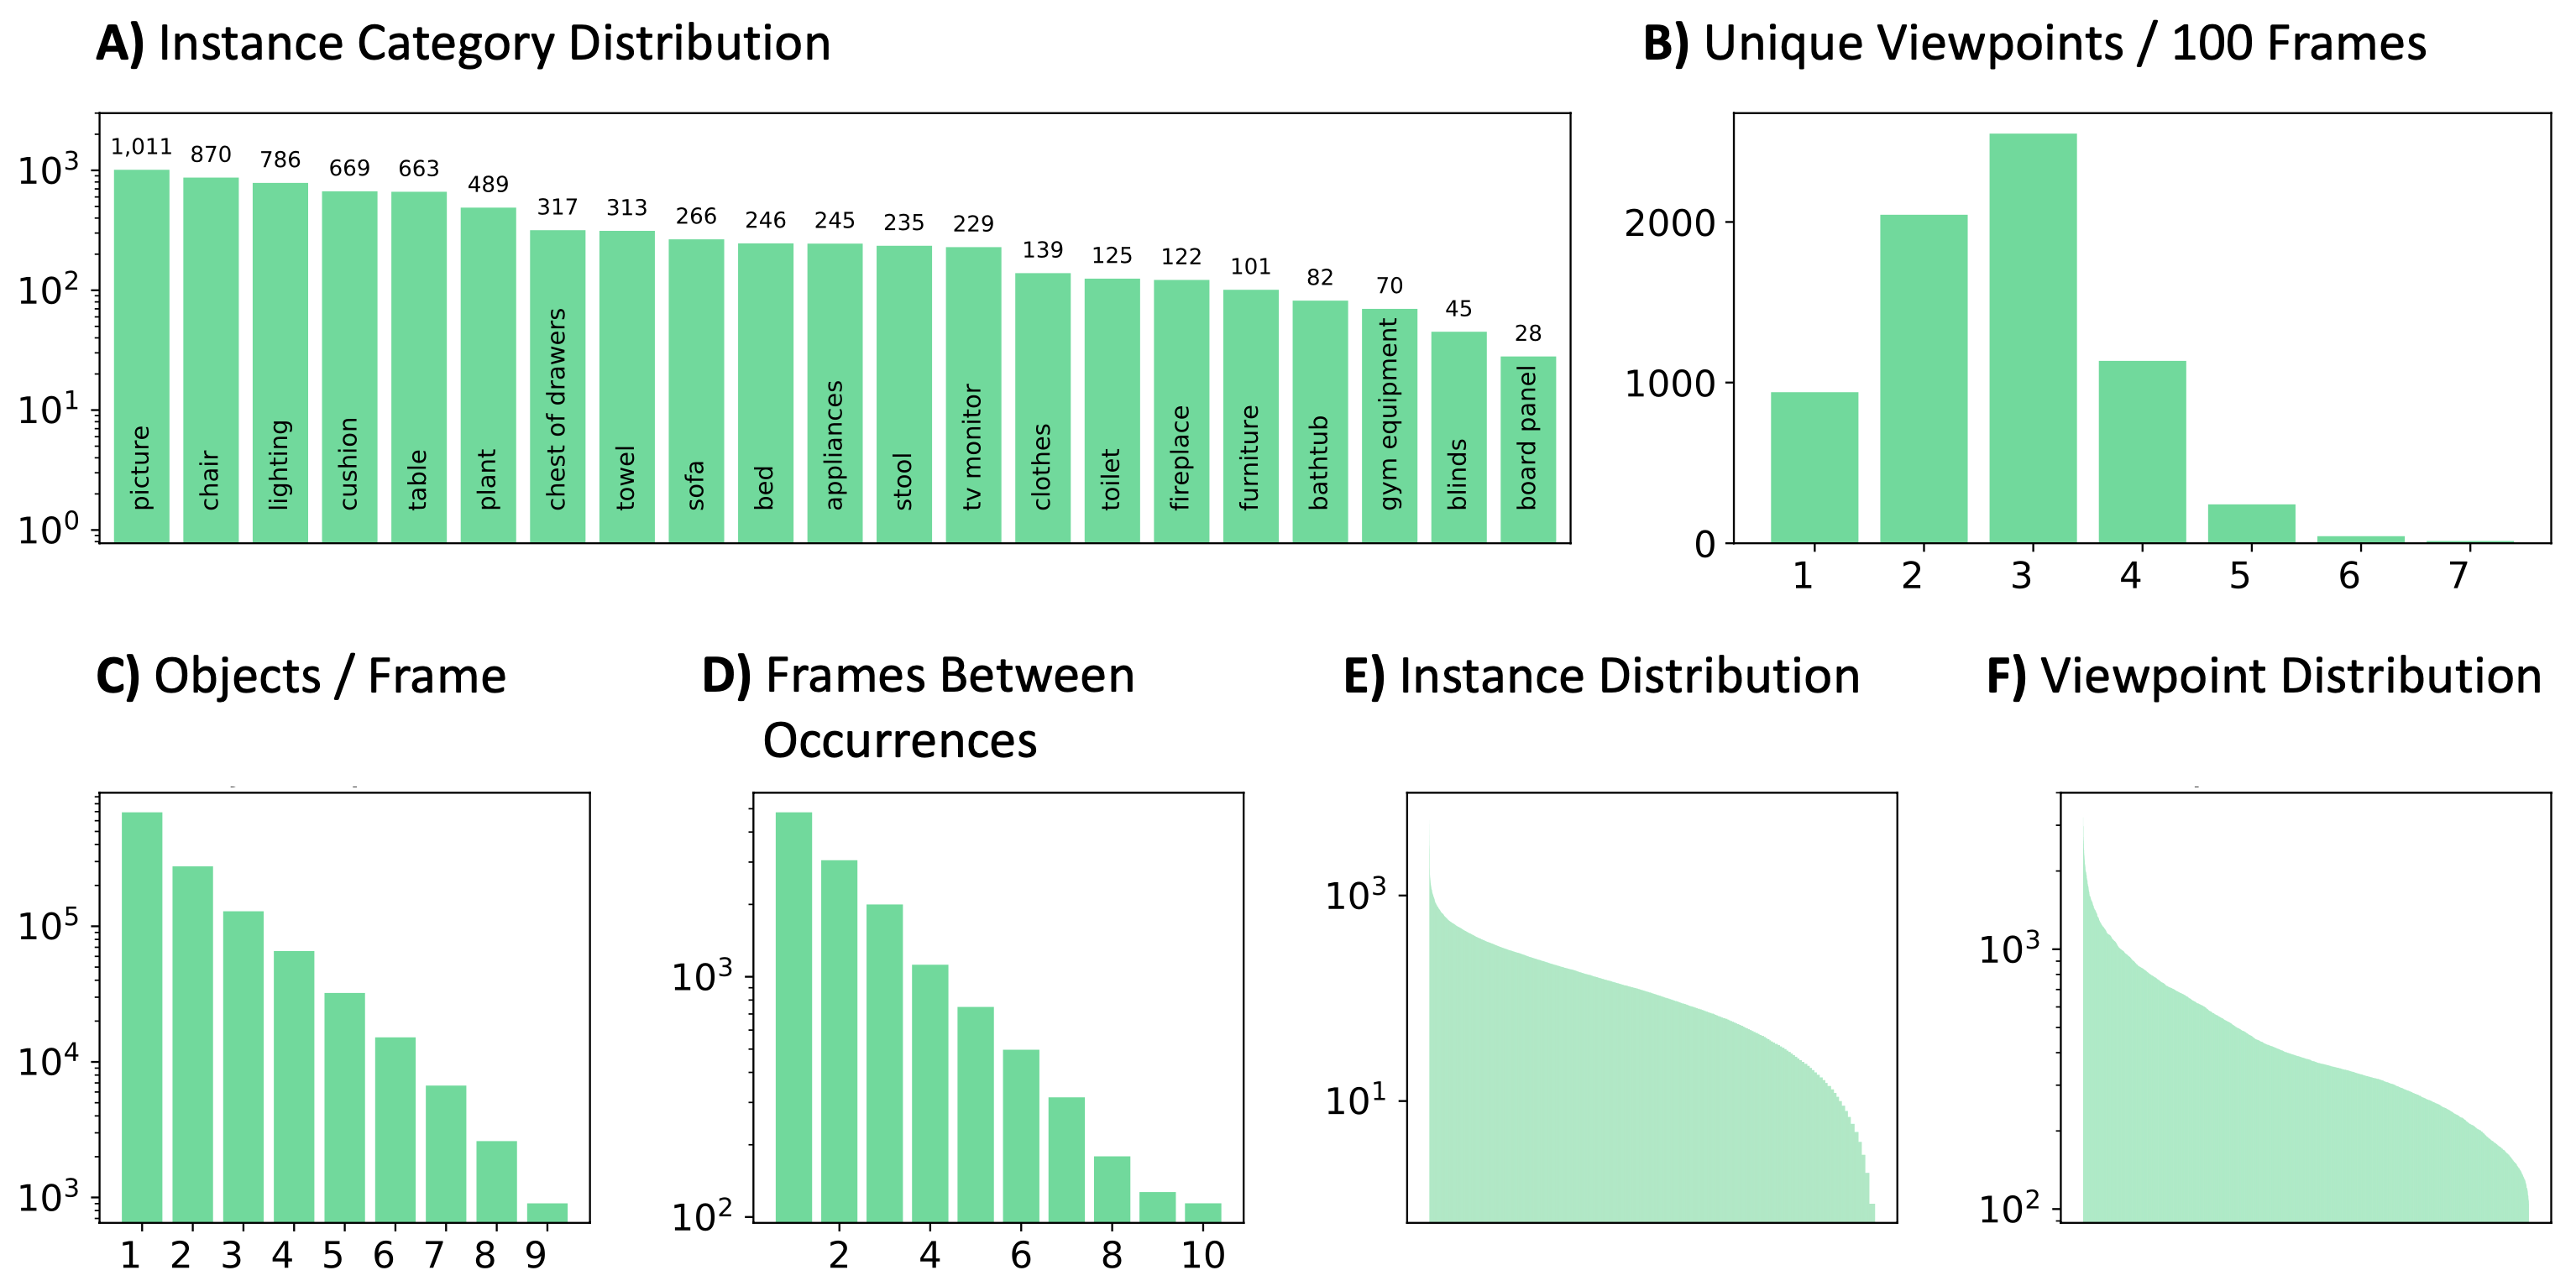
\includegraphics[width=6\textwidth]{figures/statsfull.png}
\else
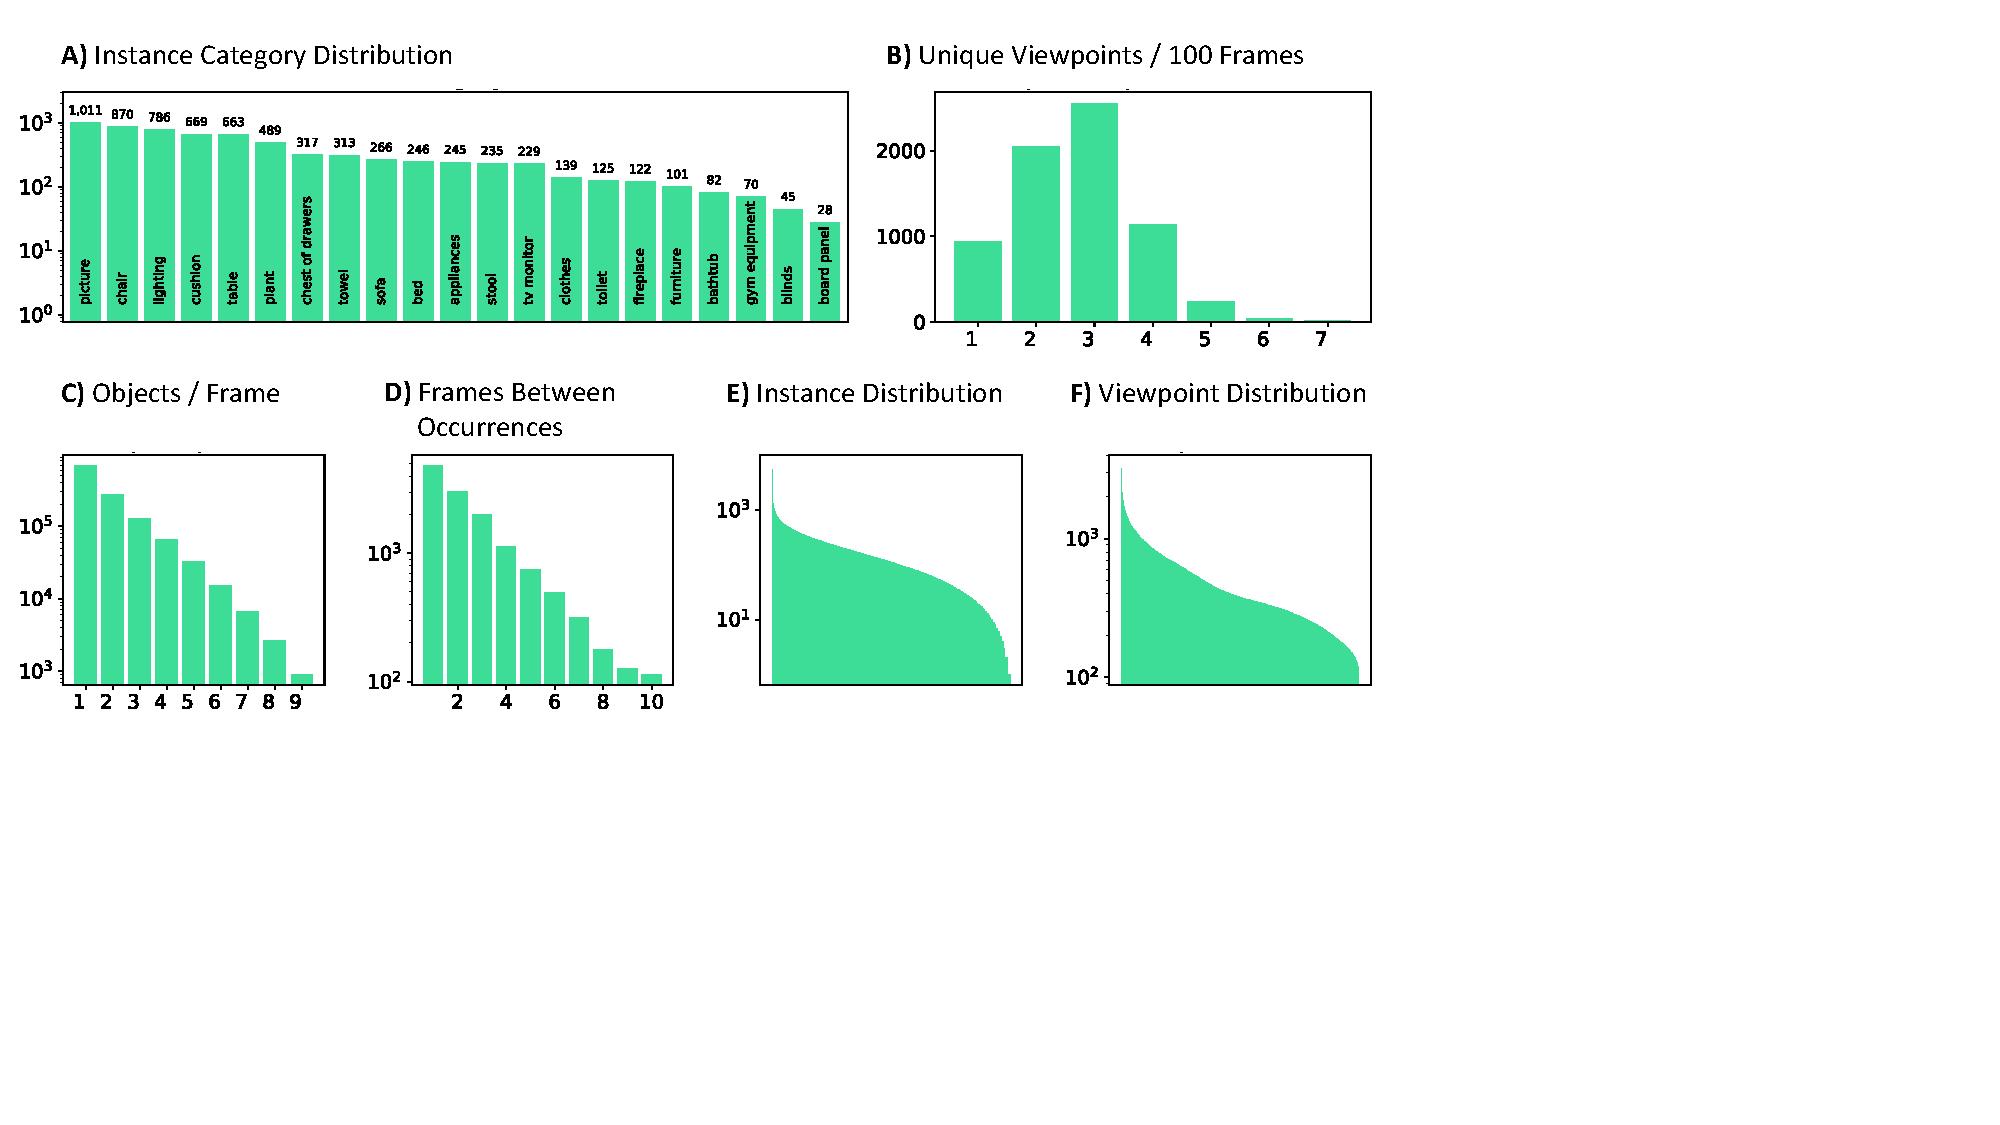
\includegraphics[width=0.9\textwidth,trim={0cm 7cm 10.2cm 0cm},clip]{figures/statsfull.pdf}
\fi
\caption{Additional statistics about our \ourroom{} dataset.}
\label{fig:additionalstats}
\end{figure}


\subsection{Training Procedure}
We use the Adam optimizer~\citep{adam} for all of our experiments, with a gradient cap of 5.0. For
\ourchar{} we train the network for 40k steps with a batch size 32 and maximum sequence length 150
across 2 GPUs and an initial learning rate 2e-3 decayed by 0.1$\times$ at 20k and 30k steps. For
\ourroom{} we train for 20k steps with a batch size 8 and maximum sequence length 100 across 4 GPUs
and an initial learning rate 1e-3 decayed by 0.1$\times$ at 8k and 16k steps. We use the BCE coefficient
$\lambda=1$  for all experiments. In semi-supervised experiments, around 30\% examples are labeled when the number of examples grows large ($\alpha = 0.3$, see Equation~\ref{eq:semisup}). Early stopping is used in \ourroom{} experiments
where the checkpoint with the highest validation AP score is chosen.
For \ourroom{}, we sample Bernoulli sequences on unlabeled inputs to 
gradually allow semi-supervised writing to the prototype memory and we find it helps training stability. The probability starts with 0.0 and increase by 0.2 every 2000 training steps until reaching 1.0.

\subsection{Data Augmentation}
For \ourchar{}, we pad the 28$\times$28 image to 32$\times$32 and then apply random cropping.

For \ourroom{}, we apply random cropping in the time dimension to get a chunk of 100 frames per
input example. We also apply random dropping of 5\% of the frames. We pad the 120$\times$160 images
to 126 $\times$ 168 and apply random cropping in each image frame. We also randomly flip the order
of the sequence (going forward or backward).


\subsection{Spatiotemporal context experiment details}
We use the Kylberg texture dataset~\citep{uppsala} without rotations. Texture classes are split into train, val, and test, defined in Table~\ref{tab:uppsalasplit}. We resize all images first to 256$\times$256. For each Omniglot image, a 28$\times$28 patch is randomly cropped from a texture image to serve as background. Random Gaussian noises with mean zero and standard deviation 0.1 are added to the background images.

For spatial background experiments, we added an additional learnable network of the same size as the main network to take the background image as input, and output the same sized embedding vector. This embedding vector is further concatenated with the main embedding vector to form the final embedding of the input. We also found that using spatially overlayed images with a single CNN can achieve similar performance as well. The final numbers are reported using the concatenation approach since it is less prone to overlay noises and is more similar to the implementation we use in the RoamingRooms experiments.

% !TEX root = ../supp.tex
\iflatexml
    \begin{table}[t]
    \begin{tabular}{clllll}
    \toprule

    \mr{3}{Train} &
    \texttt{blanket2} &
    \texttt{ceiling2} &
    \texttt{floor2} &
    \texttt{grass1} &
    \texttt{linseeds1} \\
    &
    \texttt{pearlsugar1} &
    \texttt{rice2} &
    \texttt{scarf2} &
    \texttt{screen1} &
    \texttt{seat2} \\
    &
    \texttt{sesameseeds1} &
    \texttt{stone1} & 
    \texttt{stoneslab1} & &
    \\
    \midrule

    \mr{2}{Val} &
    \texttt{blanket1} &
    \texttt{canvas1} &
    \texttt{ceiling1} & 
    \texttt{floor1} &
    \texttt{scarf1} \\
    &
    \texttt{rice1} &
    \texttt{stone2} & & & \\
    \midrule
    \mr{2}{Test} & 
    \texttt{wall1} &
    \texttt{lentils1} & 
    \texttt{cushion1} &
    \texttt{rug1} &
    \texttt{sand1} \\
    &
    \texttt{oatmeal1} &
    \texttt{stone3} &
    \texttt{seat1} & & \\
    \bottomrule
    \end{tabular}
    \caption{\textbf{Split information for the Kylberg texture dataset}. Each column is an texture type. Rows are continuation of lines.}
    \label{tab:uppsalasplit}
    \end{table}
\else
    \begin{table}[t]
    \vspace{-0.5in}
    \caption{\textbf{Split information for the Kylberg texture dataset}. Each column is an texture type. Rows are continuation of lines.}
    \label{tab:uppsalasplit}
    \begin{center}
    \begin{small}
    \begin{tabular}{clllll}
    \toprule

    \mr{3}{Train} &
    \texttt{blanket2} &
    \texttt{ceiling2} &
    \texttt{floor2} &
    \texttt{grass1} &
    \texttt{linseeds1} \\
    &
    \texttt{pearlsugar1} &
    \texttt{rice2} &
    \texttt{scarf2} &
    \texttt{screen1} &
    \texttt{seat2} \\
    &
    \texttt{sesameseeds1} &
    \texttt{stone1} & 
    \texttt{stoneslab1} & &
    \\
    \midrule

    \mr{2}{Val} &
    \texttt{blanket1} &
    \texttt{canvas1} &
    \texttt{ceiling1} & 
    \texttt{floor1} &
    \texttt{scarf1} \\
    &
    \texttt{rice1} &
    \texttt{stone2} & & & \\
    \midrule
    \mr{2}{Test} & 
    \texttt{wall1} &
    \texttt{lentils1} & 
    \texttt{cushion1} &
    \texttt{rug1} &
    \texttt{sand1} \\
    &
    \texttt{oatmeal1} &
    \texttt{stone3} &
    \texttt{seat1} & & \\
    \bottomrule
    \end{tabular}
    \end{small}
    \end{center}
    \end{table}
 \fi


\subsection{Baseline implementation details}
\paragraph{Online meta-learning (OML):} The OML  model performs one gradient descent step for each
input. In order for the model to predict unknown, we use the probability output from the softmax
layer summing across the unused units. For example, if the softmax layer has 40 units and we have
only seen 5 classes so far, then we sum the probability from the 6th to the last units. This summed
probability is separately trained with a binary cross entropy, same as in Equation~\ref{eq:loss}.

The inner learning rate is set to 1e-2 and we truncate the number of unrolled gradient descent steps
to 5/20 (\ourchar{}/\ourroom{}), in order to make the computation feasible. For \ourchar{}, the
network is trained with a batch size 32 across 2 GPUs, for a total of 20k steps, with an initial
learning rate 2e-3 decayed by 0.1 at 10k and 16.7k steps. For \ourroom{}, the network is trained
with a batch size 8 across 4 GPUs, for a total of 16k steps, with an initial learning rate 1e-3
decayed by 0.1 at 6.4k and 12.8k steps.

\paragraph{Long short-term memory (LSTM):} We apply a stacked two layer LSTM with 256 hidden
dimensions. Inputs are $\bh_t^{\text{CNN}}$ concatenated with the label one-hot vector. If an
example is unlabeled, then the label vector is all-zero. We directly apply a linear layer on top of
the LSTM to map the LSTM memory output into classification logits, and the last logit is the binary
classification logit reserved for unknown. The training procedure is the same as our CPM model.

\paragraph{Differentiable neural computer (DNC):} In order to make the DNC model work properly, we
found that it is sometimes helpful to pretrain the CNN weights. Simply initializing from scratch and
train CNN+DNC end-to-end sometimes results in poor performance. We hypothesize that the attention
structure in the DNC model is detrimental to representation learning. Therefore, for \ourchar{}
experiments, we use pretrained ProtoNet weights for solving 1-shot 5-way episodes to initialize the
CNN, and we keep finetuning the CNN weights with 10\% of the full learning rate. For \ourroom{}
experiments, we train the full model end-to-end from scratch.

The DNC is also modified so that it is more effective using the label information from the input. In
the original MANN paper~\citep{mann} for one-shot learning, the input features $\bh_t^{\text{CNN}}$
and the label one-hot ID are simply concatenated to feed into the LSTM controller of MANN. We find
that it is beneficial to directly add label one-hot vector as an input to the write head that
generates the write attention and the write content.  Similar to the LSTM model, the memory readout is also sent to a
linear layer in order to get the final classification logits, and the last logit is the binary
classification logit reserved for the unknowns. Finally we remove the linkage prediction part of the DNC
due to training instability.

The controller LSTM has 256 hidden dimensions, and the memory has 64 slots each with 64 dimensions.
There are 4 read heads and 4 write heads. The training procedure is the same as CPM.

\paragraph{Online ProtoNet:} Online ProtoNet is our modification of the original
ProtoNet~\citep{protonet}. It is similar to our CPM model without the contextual RNN. The feature
from the CNN is directly written to the prototype memory. In addition, we do not predict the control
hyperparameters $\beta^{\{r,w\}}_t,\gamma^{\{r,w\}}_t$ from the RNN and they are learned as regular parameters. The training procedure is the same as CPM.

\paragraph{Online MatchingNet:} Online MatchingNet is our modification of the original
MatchingNet~\citep{matchingnet}. We do not consider the context embedding in the MatchingNet paper
since it was originally designed for the entire episode using an attentional RNN encoder. It is
similar to online ProtoNet but instead of doing online averaging, it directly stores each example
and its class. Since it is an example-based storage, we did not extend it to learn from
unlabeled examples, and all unlabeled examples are skipped. We use a similar decision rule to
determine whether an example belongs to a known cluster by looking at the distance to the nearest
exemplar stored in the memory, shifted by $\beta$ and scaled by $1/\gamma$. Note that online
MatchingNet is not efficient at memory storage since it scales with the number of steps in the
sequence. In addition, we use the negative Euclidean distance as the similarity function. The training
procedure is the same as CPM.

\paragraph{Online infinite mixture prototypes (IMP):} Online IMP is proposed as a mix of prototype and example-based storage by allowing a class to have multiple clusters. If an
example is classified as unknown or it is unlabeled, we will assign its cluster based on our
prediction, which either assigns it to one of the existing clusters or creates a new cluster,
depending on its distance to the nearest cluster. If a cluster with an unknown label later is
assigned with an example with a known class, then the cluster label will also be updated. We use the same
decision rule as online ProtoNet to determine whether an example belongs to a known cluster by
looking at the distance to the nearest cluster, shifted by $\beta$ and scaled by $1/\gamma$. As
described above, online IMP has the capability of learning from unlabeled examples, unlike online
MatchingNet. However similar to online MatchingNet, online IMP is also not efficient at memory
storage since in the worst case it also scales with the number of steps in the sequence. Again, the
training procedure is the same as CPM.

\section{Additional Experimental Results}
\label{sec:additionalresults}
\subsection{Effect of Forgetting}
We report the effect of forgetting of \ourroom{} and \ourimg{} in Table~\ref{tab:forgetroom} and \ref{tab:forgetimagenet}.
\iflatexml
\begin{table}[t]
    \centering
    \begin{tabular}{ccccccc|cccccc}
    \toprule
    & \mc{6}{c|}{\textbf{Supervised}} & \mc{6}{c}{\textbf{Semi-Supervised}}\\
                &   1 - 2&      3 - 5&      6 - 10&     11 - 20&    21 - 50&    51 - 100&
                    1 - 2&      3 - 5&      6 - 10&     11 - 20&    21 - 50&    51 - 100\\
    OPN 1-Shot  &   93.5&   	89.3&	    79.4&	    67.2&	    60.3&	    60.1&
                    86.5&	    83.6&	    76.3&	    68.4&	    64.7&	    61.5\\
    CPM 1-Shot  &   \bf{95.7}&	\bf{92.2}&  \bf{85.7}&	\bf{75.2}&	\bf{70.0}&  \bf{66.4}&
                    \bf{91.0}&	\bf{88.7}&	\bf{82.9}&	\bf{77.0}&  \bf{72.2}&	\bf{66.5}\\
    OPN 3-Shot  &   95.1&	    91.8&	    85.6&   	78.2&	    74.6&	    73.8&
                    92.6&       88.0&	    85.1&	    81.1&	    80.6&	    76.7\\
    CPM 3-Shot  &   \bf{96.1}&	\bf{93.8}&	\bf{87.7}&	\bf{81.4}&  \bf{79.1}&	\bf{78.2}&
                    \bf{94.8}&  \bf{91.0}&	\bf{86.9}&	\bf{83.1}&	\bf{82.7}&  \bf{79.2}\\
    \bottomrule
    \end{tabular}
    \caption{\textbf{Effect of forgetting over a time interval on \ourroom{}.} Average accuracy vs. the number of time steps since the model has last seen the label of a particular class.}
    \label{tab:forgetroom}
\end{table}

\begin{table}[t]
    \centering
    \begin{tabular}{ccccccc|cccccc}
    \toprule
    & \mc{6}{c|}{\bf Supervised} & \mc{6}{c}{\bf Semi-Supervised}\\
                &   1 - 2&      3 - 5&      6 - 10&     11 - 20&    21 - 50&    51 - 100&
                    1 - 2&      3 - 5&      6 - 10&     11 - 20&    21 - 50&    51 - 100\\
    OPN 1-Shot  &   40.8&	35.9&	33.0&	\bf{30.7}&	\bf{27.0}&	\bf{21.4}&
                    40.5&	37.7&	35.9&	\bf{33.7}&	\bf{31.5}&	\bf{28.4}\\
    CPM 1-Shot  &   \bf{67.5}&	\bf{52.9}&	\bf{35.5}&	24.2&	18.3&	13.8&
                    \bf{60.4}&	\bf{51.3}&	\bf{39.5}&	26.6&	21.8&	15.4\\
    OPN 3-Shot  &   52.5&	50.3&	\bf{48.8}&	\bf{47.2}&	\bf{44.4}&	\bf{42.3}&
                    57.6&	55.1&	\bf{54.6}&	\bf{52.3}&	\bf{52.1}&	\bf{49.5}\\
    CPM 3-Shot  &   \bf{77.8}&	\bf{64.5}&	46.6&	32.9&	24.7&	17.9&
                    \bf{76.1}&	\bf{61.8}&	48.6&	30.5&	24.1&	15.6\\
    \bottomrule
    \end{tabular}
    \caption{\textbf{Effect of forgetting over a time interval on \ourimg{}.} Average accuracy vs. the number of time steps since the model has last seen the label of a particular class.}
    \label{tab:forgetimagenet}
\end{table}

\else
\begin{table}[t]
\vspace{-0.5in}
    \centering
    \caption{\textbf{Effect of forgetting over a time interval on \ourroom{}.} Average accuracy vs. the number of time steps since the model has last seen the label of a particular class.}
    
    \resizebox{\textwidth}{!}{
    \begin{tabular}{ccccccc|cccccc}
    \toprule
    & \mc{6}{c}{\bf Supervised} & \mc{6}{c}{\bf Semi-Supervised}\\
                &   1 - 2&      3 - 5&      6 - 10&     11 - 20&    21 - 50&    51 - 100&
                    1 - 2&      3 - 5&      6 - 10&     11 - 20&    21 - 50&    51 - 100\\
    \midrule
    OPN 1-Shot  &   93.5&   	89.3&	    79.4&	    67.2&	    60.3&	    60.1&
                    86.5&	    83.6&	    76.3&	    68.4&	    64.7&	    61.5\\
    CPM 1-Shot  &   \bf{95.7}&	\bf{92.2}&  \bf{85.7}&	\bf{75.2}&	\bf{70.0}&  \bf{66.4}&
                    \bf{91.0}&	\bf{88.7}&	\bf{82.9}&	\bf{77.0}&  \bf{72.2}&	\bf{66.5}\\
    \midrule
    OPN 3-Shot  &   95.1&	    91.8&	    85.6&   	78.2&	    74.6&	    73.8&
                    92.6&       88.0&	    85.1&	    81.1&	    80.6&	    76.7\\
    CPM 3-Shot  &   \bf{96.1}&	\bf{93.8}&	\bf{87.7}&	\bf{81.4}&  \bf{79.1}&	\bf{78.2}&
                    \bf{94.8}&  \bf{91.0}&	\bf{86.9}&	\bf{83.1}&	\bf{82.7}&  \bf{79.2}\\
    \bottomrule
    \end{tabular}}
    \label{tab:forgetroom}
\end{table}

\begin{table}[t]
\vspace{-0.2in}
    \centering
    \caption{\textbf{Effect of forgetting over a time interval on \ourimg{}.} Average accuracy vs. the number of time steps since the model has last seen the label of a particular class.}
    
    \resizebox{\textwidth}{!}{
    \begin{tabular}{ccccccc|cccccc}
    \toprule
    & \mc{6}{c}{\bf Supervised} & \mc{6}{c}{\bf Semi-Supervised}\\
                &   1 - 2&      3 - 5&      6 - 10&     11 - 20&    21 - 50&    51 - 100&
                    1 - 2&      3 - 5&      6 - 10&     11 - 20&    21 - 50&    51 - 100\\
    \midrule
    OPN 1-Shot  &   40.8&	35.9&	33.0&	\bf{30.7}&	\bf{27.0}&	\bf{21.4}&
                    40.5&	37.7&	35.9&	\bf{33.7}&	\bf{31.5}&	\bf{28.4}\\
    CPM 1-Shot  &   \bf{67.5}&	\bf{52.9}&	\bf{35.5}&	24.2&	18.3&	13.8&
                    \bf{60.4}&	\bf{51.3}&	\bf{39.5}&	26.6&	21.8&	15.4\\
    \midrule
    OPN 3-Shot  &   52.5&	50.3&	\bf{48.8}&	\bf{47.2}&	\bf{44.4}&	\bf{42.3}&
                    57.6&	55.1&	\bf{54.6}&	\bf{52.3}&	\bf{52.1}&	\bf{49.5}\\
    CPM 3-Shot  &   \bf{77.8}&	\bf{64.5}&	46.6&	32.9&	24.7&	17.9&
                    \bf{76.1}&	\bf{61.8}&	48.6&	30.5&	24.1&	15.6\\
    \bottomrule
    \end{tabular}}
    \label{tab:forgetimagenet}
\end{table}


% \subsection{Video Visualization}
% We include video visualization of \ourroom{} sequences here:
% \footnote{\url{https://drive.google.com/drive/folders/1gBJBFdNb0EOvK6CEYKxIL1Og0_jrqrbK}}. Our CPM
% model prediction can be found here:
% \footnote{\url{https://drive.google.com/drive/folders/1rp9xxAccrZyffngFdtoS9Bl6P9uxJ9xN}}.

\subsection{Embedding Visualization} 
Figure~\ref{fig:tsne} shows the learned embedding of each example in Online ProtoNet vs. our CPM
model in \ourchar{} sequences, where colors indicate environment IDs. In Online ProtoNet, the
example features does not reflect the temporal context, and as a result, colors are scattered across
the space. By contrast, in the CPM embedding visualization, colors are clustered together and we see
a smoother transition of environments in the embedding space.

% !TEX root = ../supp.tex
\begin{figure}[t]
\centering
% \vspace{-0.2in}
\iflatexml
    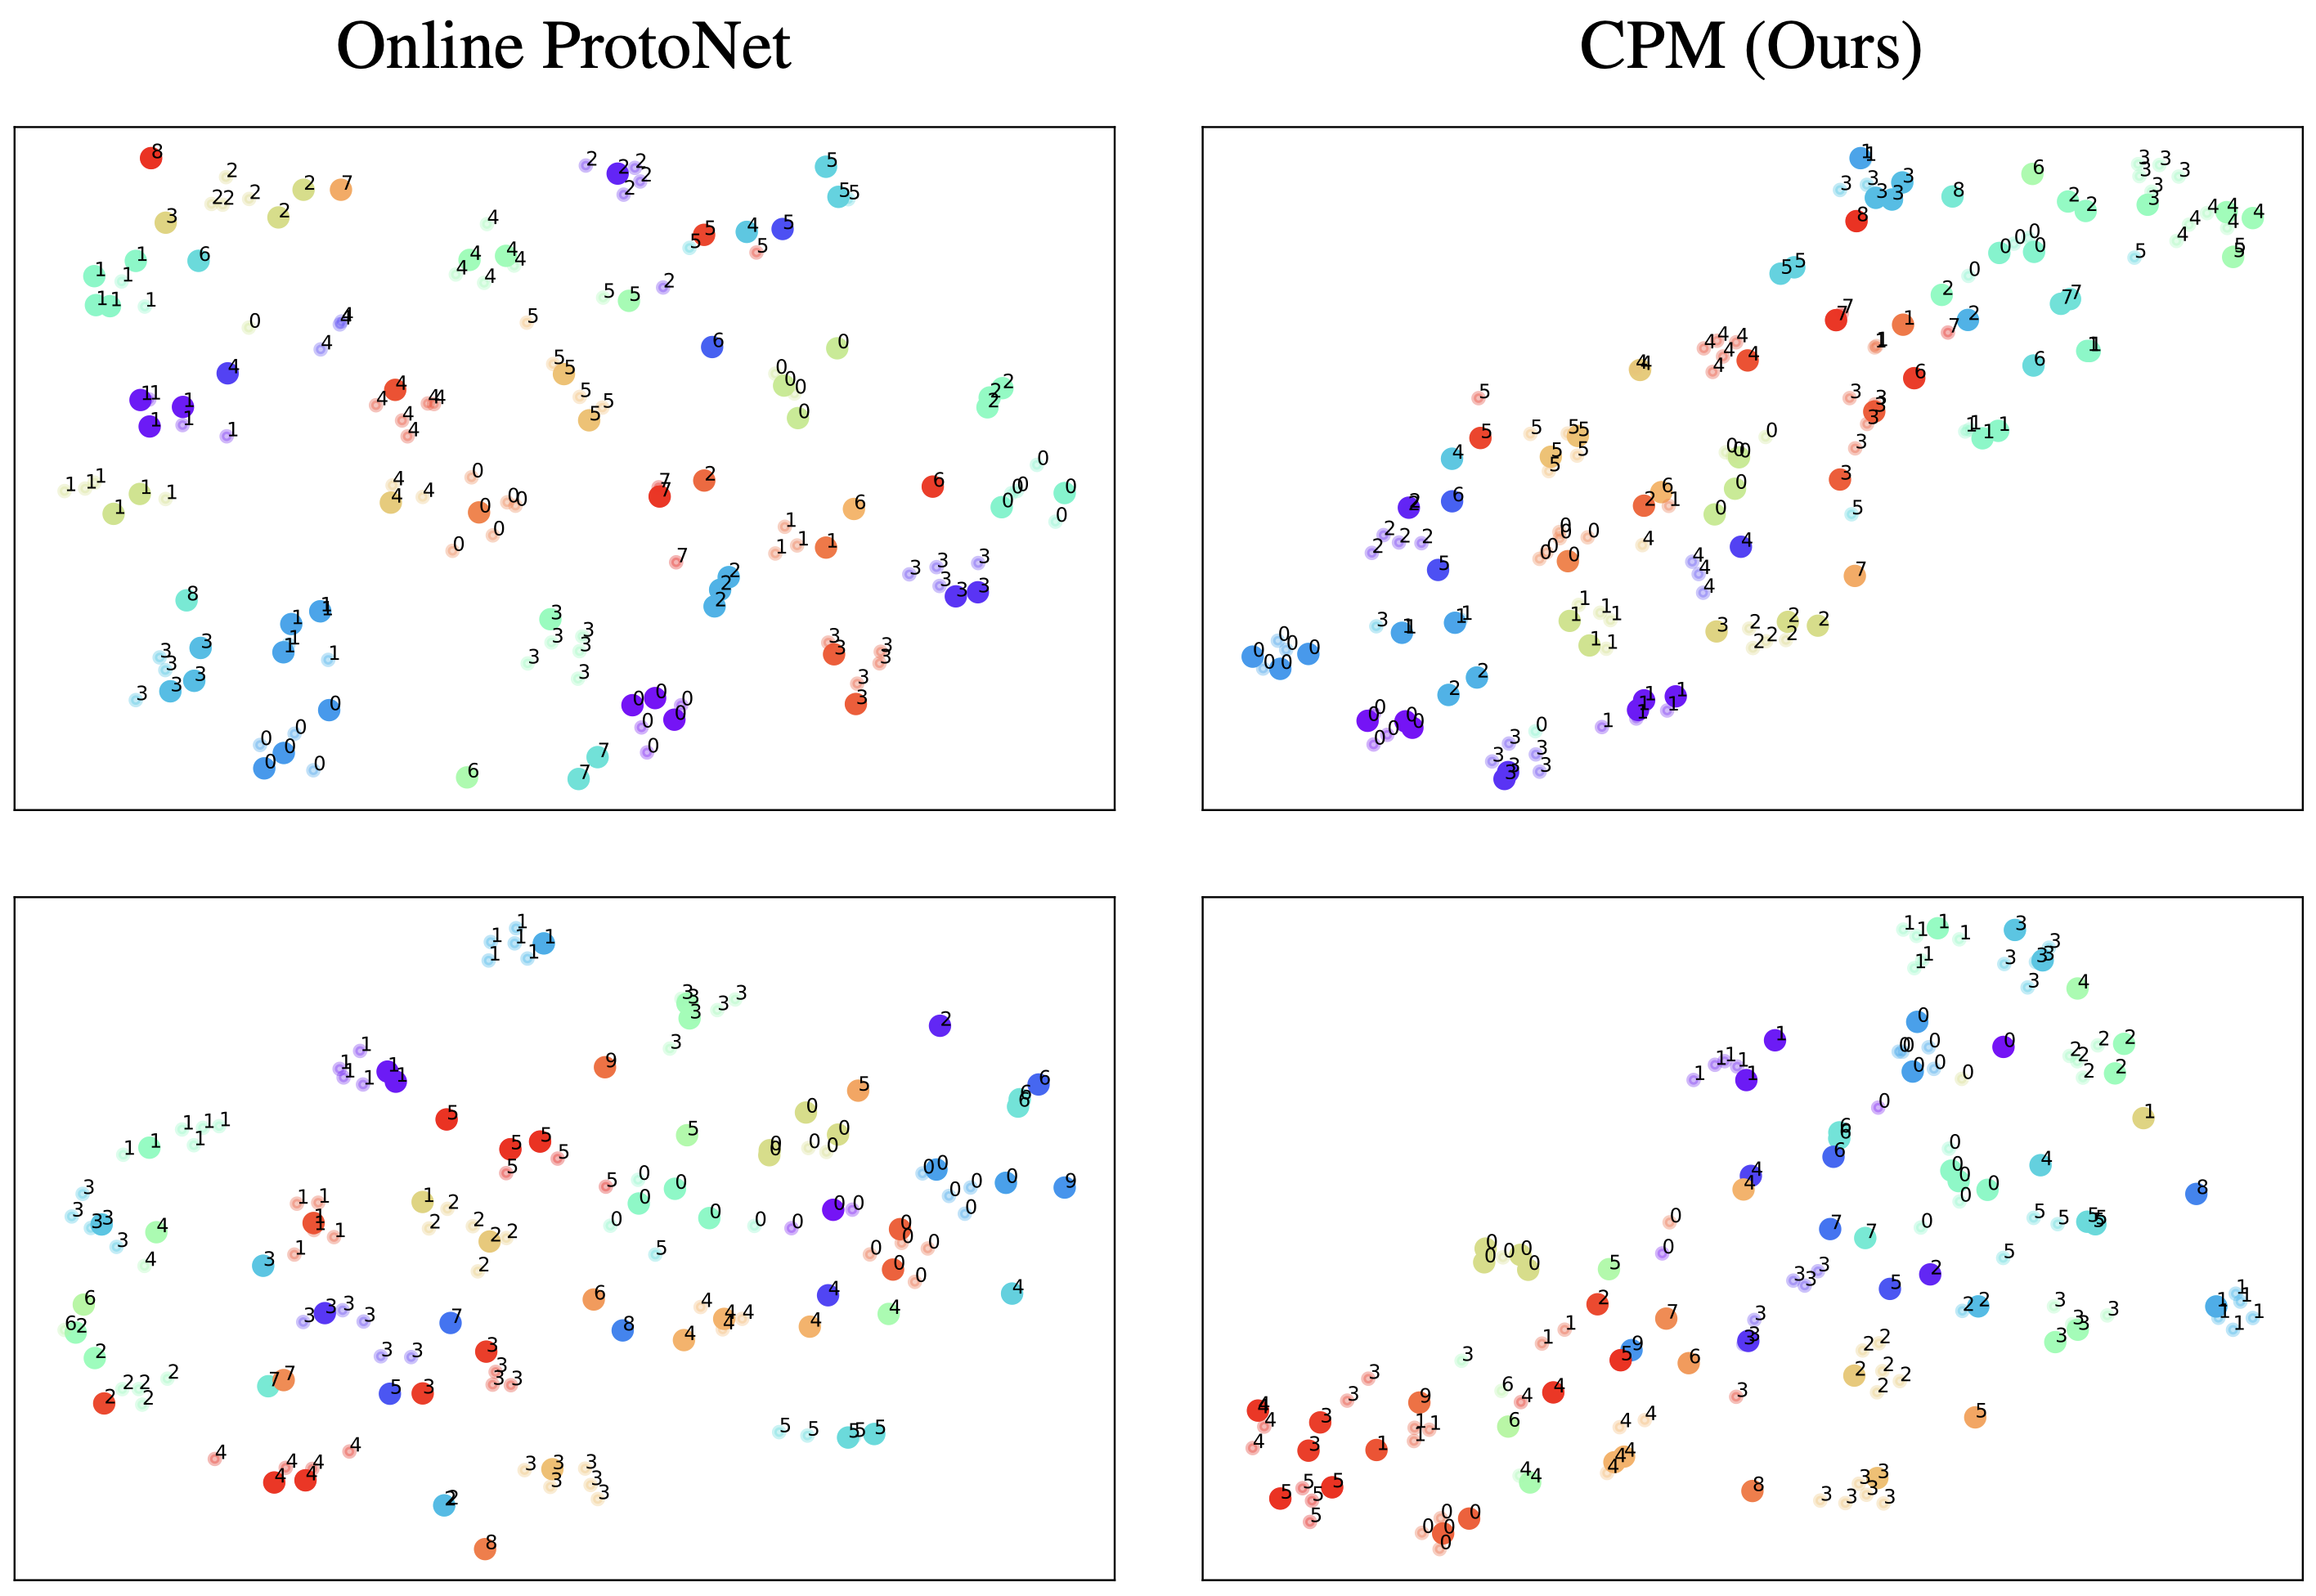
\includegraphics[width=6\linewidth]{figures/omniglot-tsne.png}
\else
    \begin{tabular}{cc}
    Online ProtoNet & CPM (Ours) \\
    \includegraphics[height=3.8cm, trim={2.5cm 1cm 2cm 1cm}, clip]{figures/omniglot-protonet-tsne/tsne-003.pdf}
    &
    \includegraphics[height=3.8cm, trim={2.5cm 1cm 2cm 1cm}, clip]{figures/omniglot-cpm-tsne/tsne-003.pdf}
    \\
    \includegraphics[height=3.8cm, trim={2.5cm 1cm 2cm 1cm}, clip]{figures/omniglot-protonet-tsne/tsne-008.pdf}
    &
    \includegraphics[height=3.8cm, trim={2.5cm 1cm 2cm 1cm}, clip]{figures/omniglot-cpm-tsne/tsne-008.pdf}
    \end{tabular}
\fi
\caption{\textbf{Embedding space visualization of \ourchar{} sequences using t-SNE~\citep{tsne}}. Different color
denotes different environments. Text labels (relative to each environment) are annotated beside the
scatter points. Unlabeled examples shown in smaller circles with lighter colors. \textbf{Left:}
Online ProtoNet; \textbf{Right:} CPM. The embeddings learned CPM model shows a smoother transition
of classes based on their temporal environments.}
\label{fig:tsne}
\end{figure}


\subsection{Control Parameters vs. Time}
Finally we visualize the control parameter values predicted by the RNN in
Figure~\ref{fig:betagamma}. We verify that we indeed need two sets of $\beta$ and $\gamma$ for read
and write operations separately as they learn different values. $\beta^w$ is smaller than $\beta^r$
which means that the network is more conservative when writing to prototypes. $\gamma^w$ grows
larger over time, which means that the network prefers a softer slope when writing to prototypes
since in the later stage the prototype memory has already stored enough content and it can grow
faster, whereas in the earlier stage, the prototype memory is more conservative to avoid embedding
vectors to be assigned to wrong clusters.

% !TEX root = ../supp.tex
\begin{figure}
\centering
% \vspace{-0.1in}
\iflatexml
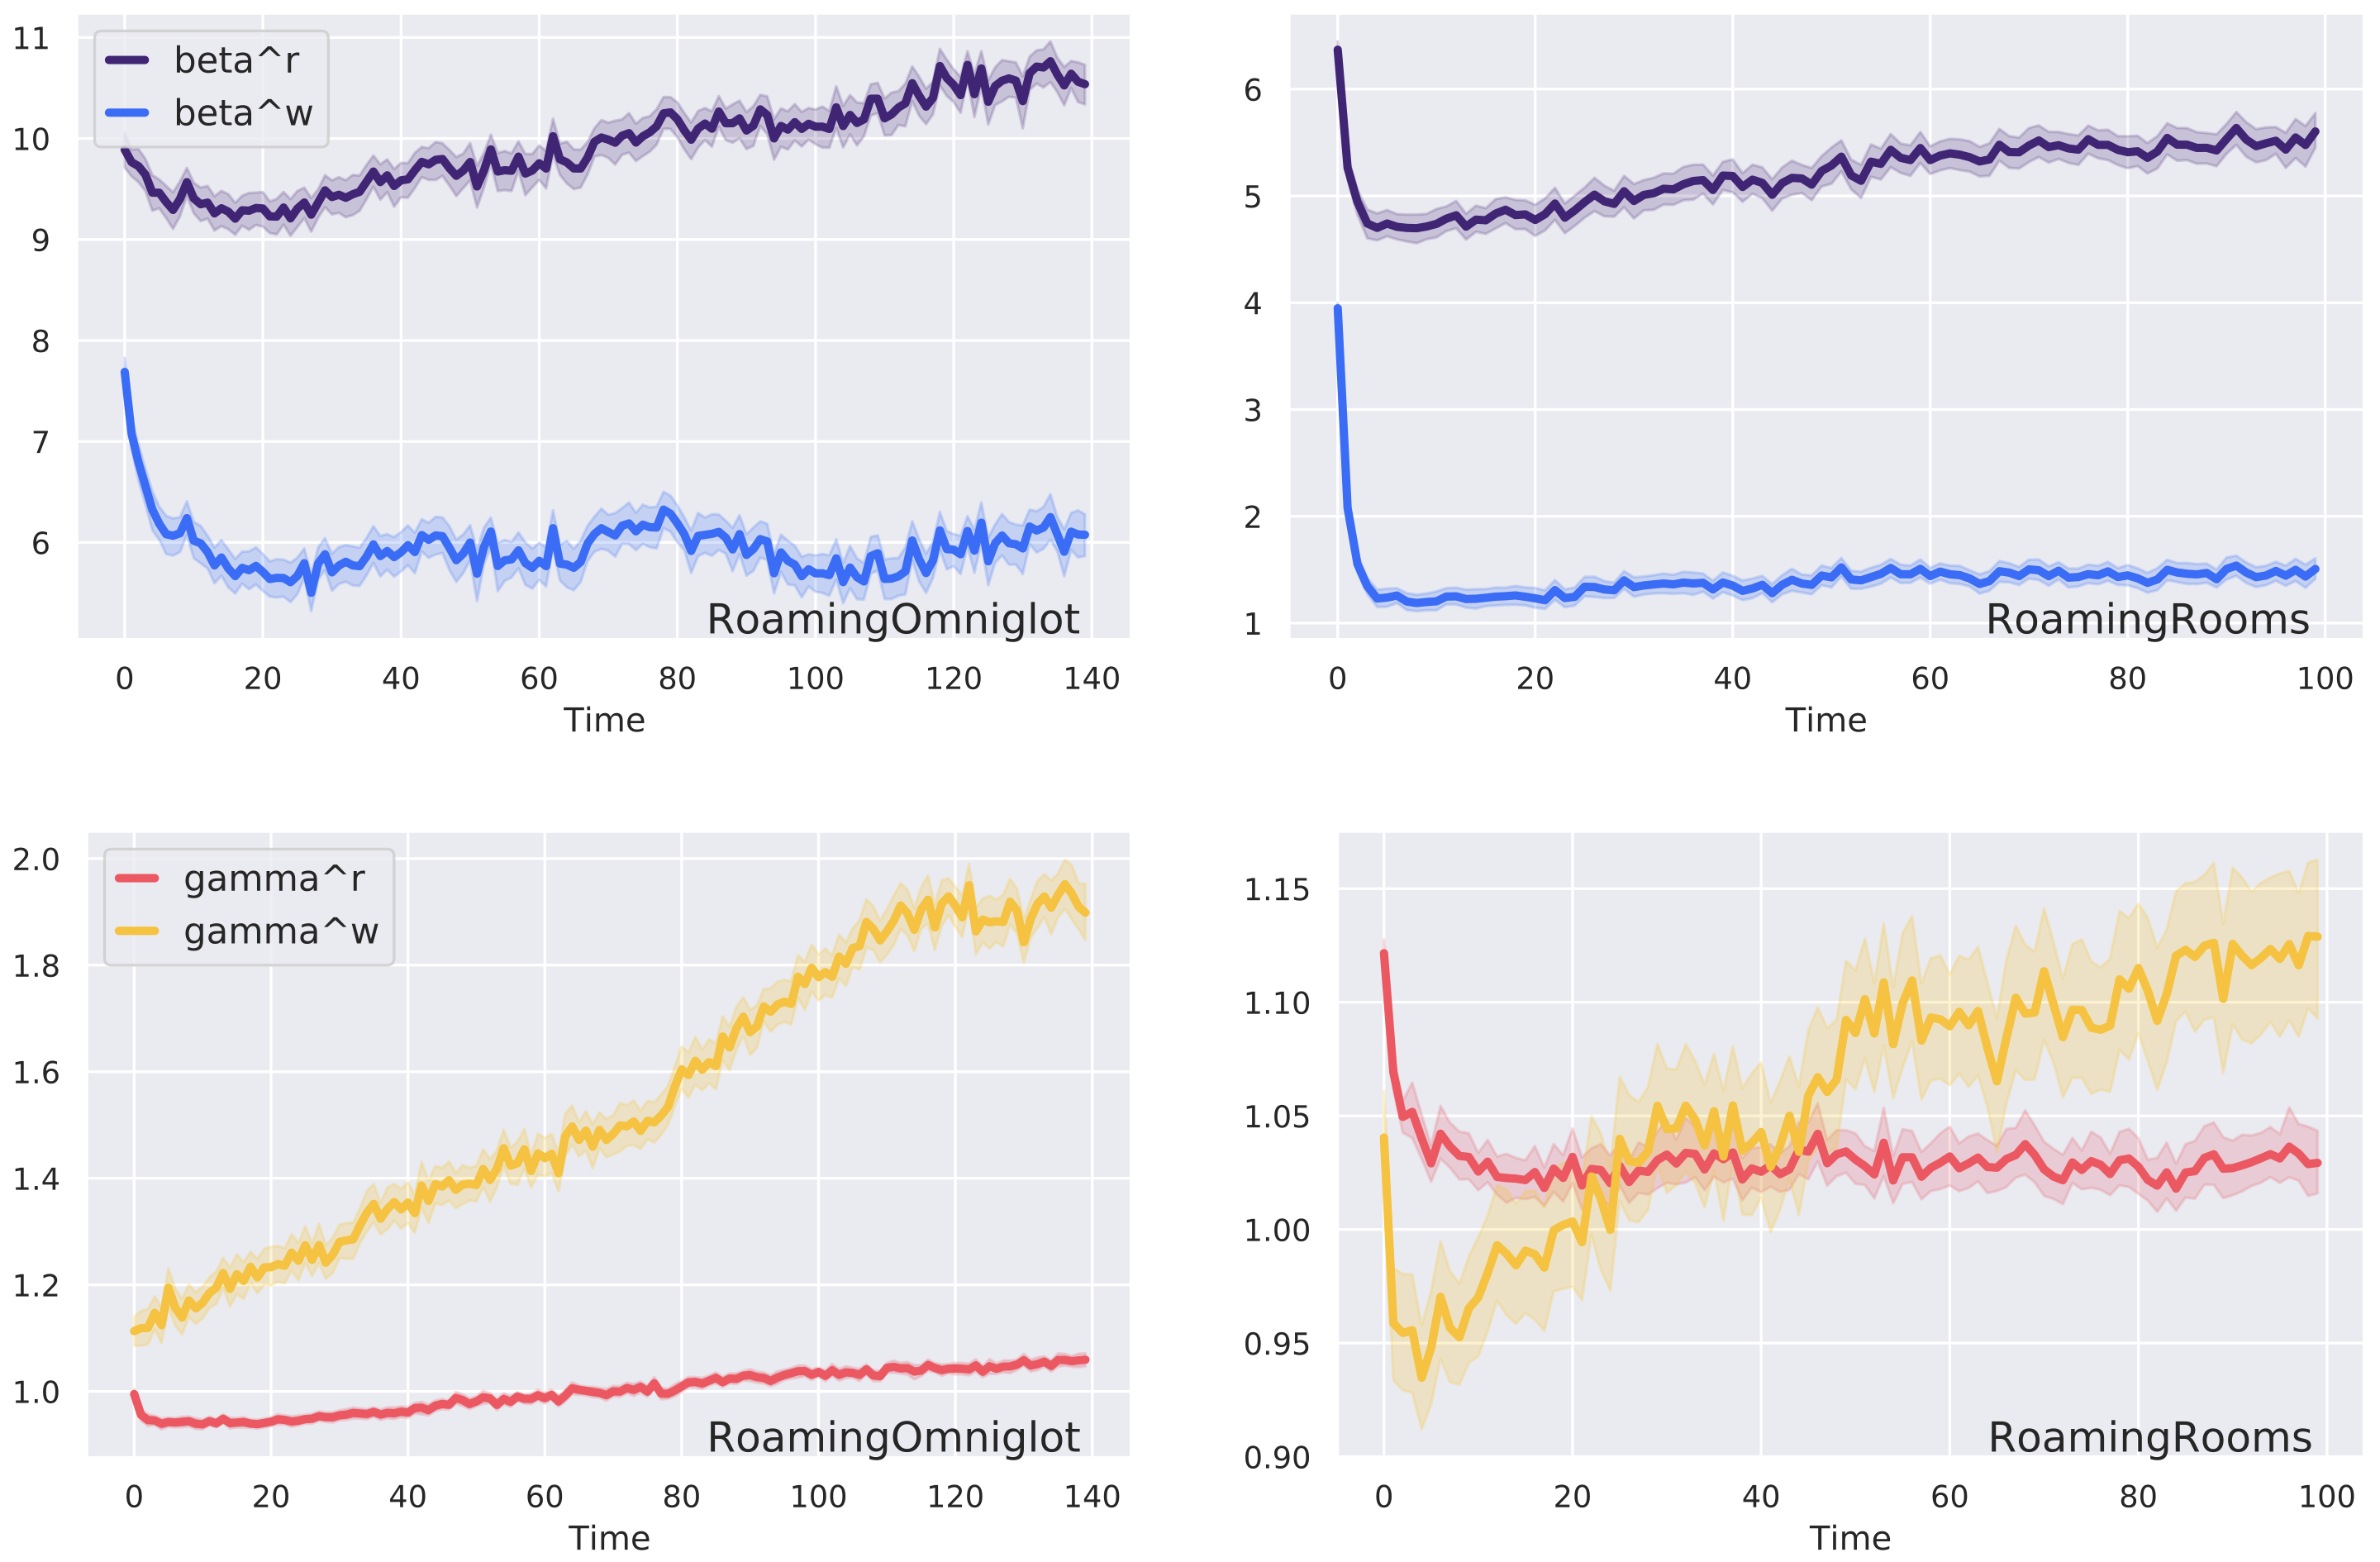
\includegraphics[width=6\linewidth]{figures/beta-gamma.png}
\else
\begin{tabular}{cc}
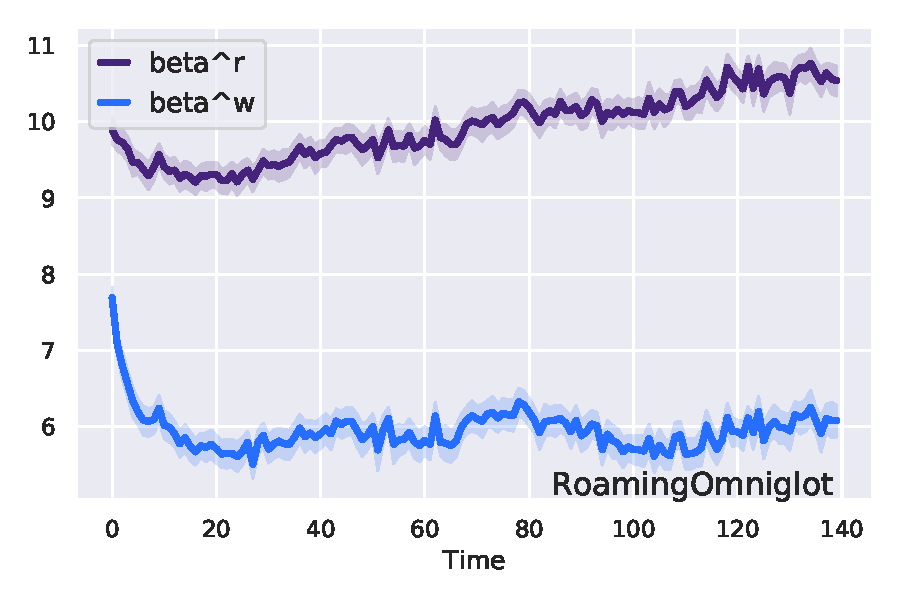
\includegraphics[height=4.0cm,trim={0.3cm 0cm 0.5cm 0},clip]{figures/omniglot-beta.pdf}
\quad
&
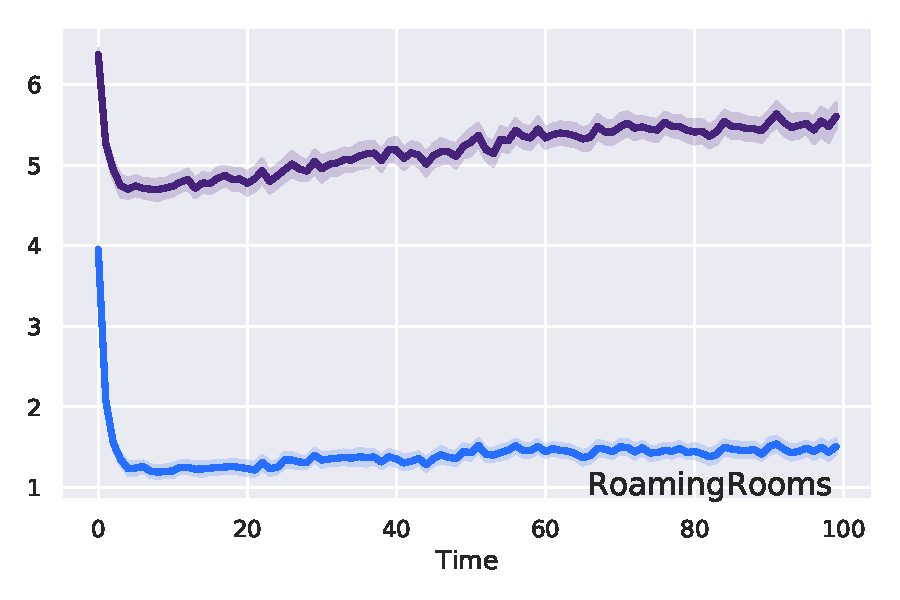
\includegraphics[height=4.0cm,trim={0.3cm 0cm 0cm 0},clip]{figures/matterport-beta.pdf}
\\
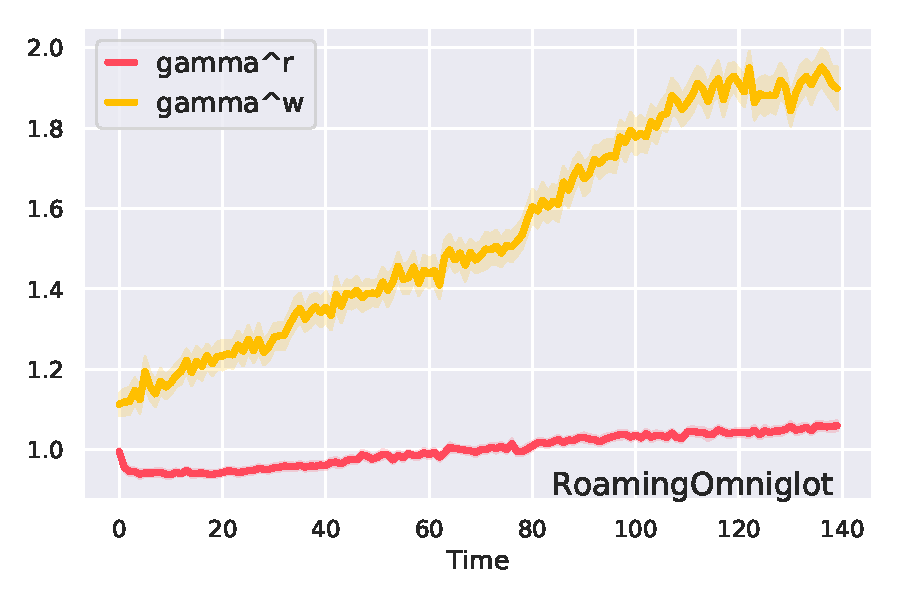
\includegraphics[height=4.0cm,trim={0.3cm 0cm 0.5cm 0},clip]{figures/omniglot-gamma.pdf}
\quad
&
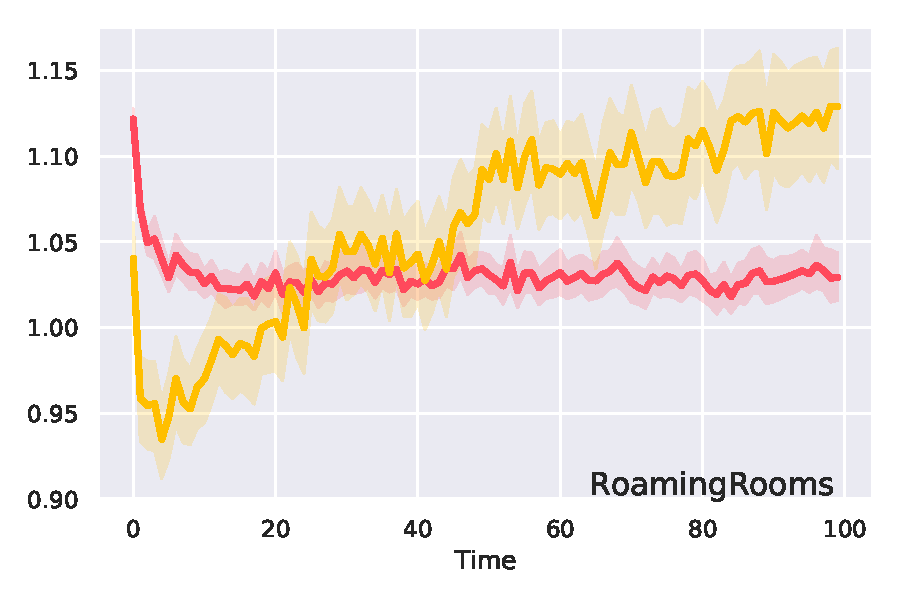
\includegraphics[height=4.0cm,trim={0.3cm 0cm 0cm 0},clip]{figures/matterport-gamma.pdf}
\\
\end{tabular}
\vspace{-0.1in}
\fi
\caption{\textbf{CPM control parameters ($\beta^{r,w}, \gamma^{r,w}$) vs. time.}
\textbf{Left:} \ourchar{} sequences; \textbf{Right:} \ourroom{} sequences; \textbf{Top:}
$\beta^{r,w}$ the threshold parameter; \textbf{Bottom:} $\gamma^{r,w}$ the temperature parameter.}
\label{fig:betagamma}
\end{figure}


\end{document}
